\documentclass[twoside]{book}

% Packages required by doxygen
\usepackage{fixltx2e}
\usepackage{calc}
\usepackage{doxygen}
\usepackage[export]{adjustbox} % also loads graphicx
\usepackage{graphicx}
\usepackage[utf8]{inputenc}
\usepackage{makeidx}
\usepackage{multicol}
\usepackage{multirow}
\PassOptionsToPackage{warn}{textcomp}
\usepackage{textcomp}
\usepackage[nointegrals]{wasysym}
\usepackage[table]{xcolor}

% Font selection
\usepackage[T1]{fontenc}
\usepackage[scaled=.90]{helvet}
\usepackage{courier}
\usepackage{amssymb}
\usepackage{sectsty}
\renewcommand{\familydefault}{\sfdefault}
\allsectionsfont{%
  \fontseries{bc}\selectfont%
  \color{darkgray}%
}
\renewcommand{\DoxyLabelFont}{%
  \fontseries{bc}\selectfont%
  \color{darkgray}%
}
\newcommand{\+}{\discretionary{\mbox{\scriptsize$\hookleftarrow$}}{}{}}

% Page & text layout
\usepackage{geometry}
\geometry{%
  a4paper,%
  top=2.5cm,%
  bottom=2.5cm,%
  left=2.5cm,%
  right=2.5cm%
}
\tolerance=750
\hfuzz=15pt
\hbadness=750
\setlength{\emergencystretch}{15pt}
\setlength{\parindent}{0cm}
\setlength{\parskip}{3ex plus 2ex minus 2ex}
\makeatletter
\renewcommand{\paragraph}{%
  \@startsection{paragraph}{4}{0ex}{-1.0ex}{1.0ex}{%
    \normalfont\normalsize\bfseries\SS@parafont%
  }%
}
\renewcommand{\subparagraph}{%
  \@startsection{subparagraph}{5}{0ex}{-1.0ex}{1.0ex}{%
    \normalfont\normalsize\bfseries\SS@subparafont%
  }%
}
\makeatother

% Headers & footers
\usepackage{fancyhdr}
\pagestyle{fancyplain}
\fancyhead[LE]{\fancyplain{}{\bfseries\thepage}}
\fancyhead[CE]{\fancyplain{}{}}
\fancyhead[RE]{\fancyplain{}{\bfseries\leftmark}}
\fancyhead[LO]{\fancyplain{}{\bfseries\rightmark}}
\fancyhead[CO]{\fancyplain{}{}}
\fancyhead[RO]{\fancyplain{}{\bfseries\thepage}}
\fancyfoot[LE]{\fancyplain{}{}}
\fancyfoot[CE]{\fancyplain{}{}}
\fancyfoot[RE]{\fancyplain{}{\bfseries\scriptsize Generated by Doxygen }}
\fancyfoot[LO]{\fancyplain{}{\bfseries\scriptsize Generated by Doxygen }}
\fancyfoot[CO]{\fancyplain{}{}}
\fancyfoot[RO]{\fancyplain{}{}}
\renewcommand{\footrulewidth}{0.4pt}
\renewcommand{\chaptermark}[1]{%
  \markboth{#1}{}%
}
\renewcommand{\sectionmark}[1]{%
  \markright{\thesection\ #1}%
}

% Indices & bibliography
\usepackage{natbib}
\usepackage[titles]{tocloft}
\setcounter{tocdepth}{3}
\setcounter{secnumdepth}{5}
\makeindex

% Hyperlinks (required, but should be loaded last)
\usepackage{ifpdf}
\ifpdf
  \usepackage[pdftex,pagebackref=true]{hyperref}
\else
  \usepackage[ps2pdf,pagebackref=true]{hyperref}
\fi
\hypersetup{%
  colorlinks=true,%
  linkcolor=blue,%
  citecolor=blue,%
  unicode%
}

% Custom commands
\newcommand{\clearemptydoublepage}{%
  \newpage{\pagestyle{empty}\cleardoublepage}%
}

\usepackage{caption}
\captionsetup{labelsep=space,justification=centering,font={bf},singlelinecheck=off,skip=4pt,position=top}

%===== C O N T E N T S =====

\begin{document}

% Titlepage & ToC
\hypersetup{pageanchor=false,
             bookmarksnumbered=true,
             pdfencoding=unicode
            }
\pagenumbering{alph}
\begin{titlepage}
\vspace*{7cm}
\begin{center}%
{\Large Rmap I2\+C-\/\+TH \\[1ex]\large 2 }\\
\vspace*{1cm}
{\large Generated by Doxygen 1.8.13}\\
\end{center}
\end{titlepage}
\clearemptydoublepage
\pagenumbering{roman}
\tableofcontents
\clearemptydoublepage
\pagenumbering{arabic}
\hypersetup{pageanchor=true}

%--- Begin generated contents ---
\chapter{Class Index}
\section{Class List}
Here are the classes, structs, unions and interfaces with brief descriptions\+:\begin{DoxyCompactList}
\item\contentsline{section}{\hyperlink{structconfiguration__t}{configuration\+\_\+t} \\*E\+E\+P\+R\+OM saved configuration }{\pageref{structconfiguration__t}}{}
\end{DoxyCompactList}

\chapter{File Index}
\section{File List}
Here is a list of all documented files with brief descriptions\+:\begin{DoxyCompactList}
\item\contentsline{section}{sketchbook/libraries/\+Digiteco\+Power/\hyperlink{digiteco__power_8cpp}{digiteco\+\_\+power.\+cpp} }{\pageref{digiteco__power_8cpp}}{}
\item\contentsline{section}{sketchbook/libraries/\+Digiteco\+Power/\hyperlink{digiteco__power_8h}{digiteco\+\_\+power.\+h} }{\pageref{digiteco__power_8h}}{}
\item\contentsline{section}{sketchbook/libraries/\+H\+Y\+T2\+X1/\hyperlink{hyt2x1_8cpp}{hyt2x1.\+cpp} }{\pageref{hyt2x1_8cpp}}{}
\item\contentsline{section}{sketchbook/libraries/\+H\+Y\+T2\+X1/\hyperlink{hyt2x1_8h}{hyt2x1.\+h} }{\pageref{hyt2x1_8h}}{}
\item\contentsline{section}{sketchbook/libraries/\+N\+T\+P/\hyperlink{ntp_8cpp}{ntp.\+cpp} }{\pageref{ntp_8cpp}}{}
\item\contentsline{section}{sketchbook/libraries/\+N\+T\+P/\hyperlink{ntp_8h}{ntp.\+h} }{\pageref{ntp_8h}}{}
\item\contentsline{section}{sketchbook/libraries/\+P\+C\+F8563/\hyperlink{pcf8563_8cpp}{pcf8563.\+cpp} }{\pageref{pcf8563_8cpp}}{}
\item\contentsline{section}{sketchbook/libraries/\+P\+C\+F8563/\hyperlink{pcf8563_8h}{pcf8563.\+h} }{\pageref{pcf8563_8h}}{}
\item\contentsline{section}{sketchbook/libraries/\+Rmap/\hyperlink{debug_8cpp}{debug.\+cpp} }{\pageref{debug_8cpp}}{}
\item\contentsline{section}{sketchbook/libraries/\+Rmap/\hyperlink{debug_8h}{debug.\+h} }{\pageref{debug_8h}}{}
\item\contentsline{section}{sketchbook/libraries/\+Rmap/\hyperlink{eeprom__utility_8h}{eeprom\+\_\+utility.\+h} }{\pageref{eeprom__utility_8h}}{}
\item\contentsline{section}{sketchbook/libraries/\+Rmap/\hyperlink{i2c__utility_8cpp}{i2c\+\_\+utility.\+cpp} }{\pageref{i2c__utility_8cpp}}{}
\item\contentsline{section}{sketchbook/libraries/\+Rmap/\hyperlink{i2c__utility_8h}{i2c\+\_\+utility.\+h} }{\pageref{i2c__utility_8h}}{}
\item\contentsline{section}{sketchbook/libraries/\+Rmap/\hyperlink{registers-rain_8h}{registers-\/rain.\+h} }{\pageref{registers-rain_8h}}{}
\item\contentsline{section}{sketchbook/libraries/\+Rmap/\hyperlink{registers-th_8h}{registers-\/th.\+h} }{\pageref{registers-th_8h}}{}
\item\contentsline{section}{sketchbook/libraries/\+Rmap/\hyperlink{registers_8h}{registers.\+h} }{\pageref{registers_8h}}{}
\item\contentsline{section}{sketchbook/libraries/\+Rmap/\hyperlink{rmap__utility_8cpp}{rmap\+\_\+utility.\+cpp} }{\pageref{rmap__utility_8cpp}}{}
\item\contentsline{section}{sketchbook/libraries/\+Rmap/\hyperlink{rmap__utility_8h}{rmap\+\_\+utility.\+h} }{\pageref{rmap__utility_8h}}{}
\item\contentsline{section}{sketchbook/libraries/\+Rmap/\hyperlink{sdcard__utility_8cpp}{sdcard\+\_\+utility.\+cpp} }{\pageref{sdcard__utility_8cpp}}{}
\item\contentsline{section}{sketchbook/libraries/\+Rmap/\hyperlink{sdcard__utility_8h}{sdcard\+\_\+utility.\+h} }{\pageref{sdcard__utility_8h}}{}
\item\contentsline{section}{sketchbook/libraries/\+Rmap/\hyperlink{stima__module_8h}{stima\+\_\+module.\+h} }{\pageref{stima__module_8h}}{}
\item\contentsline{section}{sketchbook/libraries/\+Rmap/\hyperlink{typedef_8h}{typedef.\+h} }{\pageref{typedef_8h}}{}
\item\contentsline{section}{sketchbook/libraries/\+Rmap\+Config/\hyperlink{debug__config_8h}{debug\+\_\+config.\+h} }{\pageref{debug__config_8h}}{}
\item\contentsline{section}{sketchbook/libraries/\+Rmap\+Config/\hyperlink{ethernet__config_8h}{ethernet\+\_\+config.\+h} }{\pageref{ethernet__config_8h}}{}
\item\contentsline{section}{sketchbook/libraries/\+Rmap\+Config/\hyperlink{gsm__config_8h}{gsm\+\_\+config.\+h} }{\pageref{gsm__config_8h}}{}
\item\contentsline{section}{sketchbook/libraries/\+Rmap\+Config/\hyperlink{hardware__config_8h}{hardware\+\_\+config.\+h} }{\pageref{hardware__config_8h}}{}
\item\contentsline{section}{sketchbook/libraries/\+Rmap\+Config/\hyperlink{json__config_8h}{json\+\_\+config.\+h} }{\pageref{json__config_8h}}{}
\item\contentsline{section}{sketchbook/libraries/\+Rmap\+Config/\hyperlink{lcd__config_8h}{lcd\+\_\+config.\+h} }{\pageref{lcd__config_8h}}{}
\item\contentsline{section}{sketchbook/libraries/\+Rmap\+Config/\hyperlink{mqtt__config_8h}{mqtt\+\_\+config.\+h} }{\pageref{mqtt__config_8h}}{}
\item\contentsline{section}{sketchbook/libraries/\+Rmap\+Config/\hyperlink{ntp__config_8h}{ntp\+\_\+config.\+h} }{\pageref{ntp__config_8h}}{}
\item\contentsline{section}{sketchbook/libraries/\+Rmap\+Config/\hyperlink{sdcard__config_8h}{sdcard\+\_\+config.\+h} }{\pageref{sdcard__config_8h}}{}
\item\contentsline{section}{sketchbook/libraries/\+Rmap\+Config/\hyperlink{sensors__config_8h}{sensors\+\_\+config.\+h} }{\pageref{sensors__config_8h}}{}
\item\contentsline{section}{sketchbook/libraries/\+Sensor\+Driver/\hyperlink{SensorDriver_8cpp}{Sensor\+Driver.\+cpp} }{\pageref{SensorDriver_8cpp}}{}
\item\contentsline{section}{sketchbook/libraries/\+Sensor\+Driver/\hyperlink{SensorDriver_8h}{Sensor\+Driver.\+h} }{\pageref{SensorDriver_8h}}{}
\item\contentsline{section}{sketchbook/libraries/\+Sensor\+Driver/\hyperlink{SensorDriverSensors_8h}{Sensor\+Driver\+Sensors.\+h} }{\pageref{SensorDriverSensors_8h}}{}
\item\contentsline{section}{sketchbook/libraries/sim800/\hyperlink{sim800_8cpp}{sim800.\+cpp} }{\pageref{sim800_8cpp}}{}
\item\contentsline{section}{sketchbook/libraries/sim800/\hyperlink{sim800_8h}{sim800.\+h} }{\pageref{sim800_8h}}{}
\item\contentsline{section}{sketchbook/libraries/sim800/\hyperlink{sim800Client_8h}{sim800\+Client.\+h} }{\pageref{sim800Client_8h}}{}
\item\contentsline{section}{sketchbook/rmap/{\bfseries version.\+h} }{\pageref{version_8h}}{}
\item\contentsline{section}{sketchbook/rmap/i2c-\/rain/\hyperlink{i2c-rain-config_8h}{i2c-\/rain-\/config.\+h} }{\pageref{i2c-rain-config_8h}}{}
\item\contentsline{section}{sketchbook/rmap/i2c-\/rain/\hyperlink{i2c-rain_8h}{i2c-\/rain.\+h} }{\pageref{i2c-rain_8h}}{}
\item\contentsline{section}{sketchbook/rmap/i2c-\/rain/\hyperlink{i2c-rain_8ino}{i2c-\/rain.\+ino} }{\pageref{i2c-rain_8ino}}{}
\item\contentsline{section}{sketchbook/rmap/i2c-\/th/\hyperlink{i2c-th-config_8h}{i2c-\/th-\/config.\+h} }{\pageref{i2c-th-config_8h}}{}
\item\contentsline{section}{sketchbook/rmap/i2c-\/th/\hyperlink{i2c-th_8h}{i2c-\/th.\+h} }{\pageref{i2c-th_8h}}{}
\item\contentsline{section}{sketchbook/rmap/i2c-\/th/\hyperlink{i2c-th_8ino}{i2c-\/th.\+ino} }{\pageref{i2c-th_8ino}}{}
\item\contentsline{section}{sketchbook/rmap/rmap/\hyperlink{rmap-config_8h}{rmap-\/config.\+h} }{\pageref{rmap-config_8h}}{}
\item\contentsline{section}{sketchbook/rmap/rmap/\hyperlink{rmap_8h}{rmap.\+h} }{\pageref{rmap_8h}}{}
\item\contentsline{section}{sketchbook/rmap/rmap/\hyperlink{rmap_8ino}{rmap.\+ino} }{\pageref{rmap_8ino}}{}
\end{DoxyCompactList}

\chapter{Class Documentation}
\hypertarget{structconfiguration__t}{}\section{configuration\+\_\+t Struct Reference}
\label{structconfiguration__t}\index{configuration\+\_\+t@{configuration\+\_\+t}}


E\+E\+P\+R\+OM saved configuration.  




{\ttfamily \#include $<$i2c-\/rain.\+h$>$}



Collaboration diagram for configuration\+\_\+t\+:\nopagebreak
\begin{figure}[H]
\begin{center}
\leavevmode
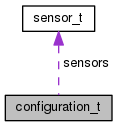
\includegraphics[width=160pt]{structconfiguration__t__coll__graph}
\end{center}
\end{figure}
\subsection*{Public Attributes}
\begin{DoxyCompactItemize}
\item 
\mbox{\Hypertarget{structconfiguration__t_a32d4c4bb78b5b231704c8a9f8d1b9e87}\label{structconfiguration__t_a32d4c4bb78b5b231704c8a9f8d1b9e87}} 
uint8\+\_\+t \hyperlink{structconfiguration__t_a32d4c4bb78b5b231704c8a9f8d1b9e87}{module\+\_\+version}
\begin{DoxyCompactList}\small\item\em module version \end{DoxyCompactList}\item 
\mbox{\Hypertarget{structconfiguration__t_a7dab895a0a9aa44bb65d90ef8016127d}\label{structconfiguration__t_a7dab895a0a9aa44bb65d90ef8016127d}} 
uint8\+\_\+t \hyperlink{structconfiguration__t_a7dab895a0a9aa44bb65d90ef8016127d}{module\+\_\+type}
\begin{DoxyCompactList}\small\item\em module type \end{DoxyCompactList}\item 
\mbox{\Hypertarget{structconfiguration__t_a0e088540266e347426ae73aed159f63a}\label{structconfiguration__t_a0e088540266e347426ae73aed159f63a}} 
uint8\+\_\+t \hyperlink{structconfiguration__t_a0e088540266e347426ae73aed159f63a}{i2c\+\_\+address}
\begin{DoxyCompactList}\small\item\em i2c address \end{DoxyCompactList}\item 
\mbox{\Hypertarget{structconfiguration__t_a227ef462f171f25e31cb3b0ce70b2597}\label{structconfiguration__t_a227ef462f171f25e31cb3b0ce70b2597}} 
bool \hyperlink{structconfiguration__t_a227ef462f171f25e31cb3b0ce70b2597}{is\+\_\+oneshot}
\begin{DoxyCompactList}\small\item\em enable or disable oneshot mode \end{DoxyCompactList}\item 
\mbox{\Hypertarget{structconfiguration__t_a33f99299576a58b3eb55be371e143531}\label{structconfiguration__t_a33f99299576a58b3eb55be371e143531}} 
bool \hyperlink{structconfiguration__t_a33f99299576a58b3eb55be371e143531}{is\+\_\+continuous}
\begin{DoxyCompactList}\small\item\em enable or disable continuous mode \end{DoxyCompactList}\item 
\mbox{\Hypertarget{structconfiguration__t_aed0a51c0dfbd925368c8539cf10c3001}\label{structconfiguration__t_aed0a51c0dfbd925368c8539cf10c3001}} 
uint8\+\_\+t \hyperlink{structconfiguration__t_aed0a51c0dfbd925368c8539cf10c3001}{i2c\+\_\+temperature\+\_\+address}
\begin{DoxyCompactList}\small\item\em i2c address of temperature sensor \end{DoxyCompactList}\item 
\mbox{\Hypertarget{structconfiguration__t_a79d1b1d9cb095c2bc0deb36c4f44452c}\label{structconfiguration__t_a79d1b1d9cb095c2bc0deb36c4f44452c}} 
uint8\+\_\+t \hyperlink{structconfiguration__t_a79d1b1d9cb095c2bc0deb36c4f44452c}{i2c\+\_\+humidity\+\_\+address}
\begin{DoxyCompactList}\small\item\em i2c address of humidity sensor \end{DoxyCompactList}\item 
\mbox{\Hypertarget{structconfiguration__t_aa003a99852a65bd2f9de0d230568bbbf}\label{structconfiguration__t_aa003a99852a65bd2f9de0d230568bbbf}} 
uint16\+\_\+t \hyperlink{structconfiguration__t_aa003a99852a65bd2f9de0d230568bbbf}{mqtt\+\_\+port}
\begin{DoxyCompactList}\small\item\em mqtt server port \end{DoxyCompactList}\item 
\mbox{\Hypertarget{structconfiguration__t_ad9a71a593cd2191ed132f9a2d6c00679}\label{structconfiguration__t_ad9a71a593cd2191ed132f9a2d6c00679}} 
char \hyperlink{structconfiguration__t_ad9a71a593cd2191ed132f9a2d6c00679}{mqtt\+\_\+server} \mbox{[}\hyperlink{mqtt__config_8h_a0a37bcf35cdbfc63d72beca198759c08}{M\+Q\+T\+T\+\_\+\+S\+E\+R\+V\+E\+R\+\_\+\+L\+E\+N\+G\+TH}\mbox{]}
\begin{DoxyCompactList}\small\item\em mqtt server \end{DoxyCompactList}\item 
\mbox{\Hypertarget{structconfiguration__t_acebf92623ad7bdf44f9707b0d99f50da}\label{structconfiguration__t_acebf92623ad7bdf44f9707b0d99f50da}} 
char \hyperlink{structconfiguration__t_acebf92623ad7bdf44f9707b0d99f50da}{mqtt\+\_\+root\+\_\+topic} \mbox{[}\hyperlink{mqtt__config_8h_a6d3b5b0f9c41b605e608f7d460491be6}{M\+Q\+T\+T\+\_\+\+R\+O\+O\+T\+\_\+\+T\+O\+P\+I\+C\+\_\+\+L\+E\+N\+G\+TH}\mbox{]}
\begin{DoxyCompactList}\small\item\em mqtt root path \end{DoxyCompactList}\item 
\mbox{\Hypertarget{structconfiguration__t_ae3699c4dd6979713472062bbad82c542}\label{structconfiguration__t_ae3699c4dd6979713472062bbad82c542}} 
char \hyperlink{structconfiguration__t_ae3699c4dd6979713472062bbad82c542}{mqtt\+\_\+subscribe\+\_\+topic} \mbox{[}\hyperlink{mqtt__config_8h_a2517f6560f7ee99813533e63d7fc91b6}{M\+Q\+T\+T\+\_\+\+S\+U\+B\+S\+C\+R\+I\+B\+E\+\_\+\+T\+O\+P\+I\+C\+\_\+\+L\+E\+N\+G\+TH}\mbox{]}
\begin{DoxyCompactList}\small\item\em mqtt subscribe topic \end{DoxyCompactList}\item 
\mbox{\Hypertarget{structconfiguration__t_ad97d47b585071f095a97296fc3e260e7}\label{structconfiguration__t_ad97d47b585071f095a97296fc3e260e7}} 
char \hyperlink{structconfiguration__t_ad97d47b585071f095a97296fc3e260e7}{mqtt\+\_\+username} \mbox{[}\hyperlink{mqtt__config_8h_a0e1860b8d036f571ffcb7e6d27832c16}{M\+Q\+T\+T\+\_\+\+U\+S\+E\+R\+N\+A\+M\+E\+\_\+\+L\+E\+N\+G\+TH}\mbox{]}
\begin{DoxyCompactList}\small\item\em mqtt username \end{DoxyCompactList}\item 
\mbox{\Hypertarget{structconfiguration__t_af842b7c625c3fdfb1b810e24fc1ba1b8}\label{structconfiguration__t_af842b7c625c3fdfb1b810e24fc1ba1b8}} 
char \hyperlink{structconfiguration__t_af842b7c625c3fdfb1b810e24fc1ba1b8}{mqtt\+\_\+password} \mbox{[}\hyperlink{mqtt__config_8h_a9fa040018ffd349e846cec27b2791fde}{M\+Q\+T\+T\+\_\+\+P\+A\+S\+S\+W\+O\+R\+D\+\_\+\+L\+E\+N\+G\+TH}\mbox{]}
\begin{DoxyCompactList}\small\item\em mqtt password \end{DoxyCompactList}\item 
\mbox{\Hypertarget{structconfiguration__t_a8de58dc10dfc6b369f34bae82426be5d}\label{structconfiguration__t_a8de58dc10dfc6b369f34bae82426be5d}} 
char \hyperlink{structconfiguration__t_a8de58dc10dfc6b369f34bae82426be5d}{ntp\+\_\+server} \mbox{[}\hyperlink{ntp__config_8h_a54153a6aa87c606f585ab167661b1be2}{N\+T\+P\+\_\+\+S\+E\+R\+V\+E\+R\+\_\+\+L\+E\+N\+G\+TH}\mbox{]}
\begin{DoxyCompactList}\small\item\em ntp server \end{DoxyCompactList}\item 
\mbox{\Hypertarget{structconfiguration__t_adede74f3da6d26f5bc4b5e64e4776f7f}\label{structconfiguration__t_adede74f3da6d26f5bc4b5e64e4776f7f}} 
\hyperlink{structsensor__t}{sensor\+\_\+t} \hyperlink{structconfiguration__t_adede74f3da6d26f5bc4b5e64e4776f7f}{sensors} \mbox{[}\hyperlink{rmap-config_8h_af18dc3de744722cb308451b7a705611b}{U\+S\+E\+\_\+\+S\+E\+N\+S\+O\+R\+S\+\_\+\+C\+O\+U\+NT}\mbox{]}
\begin{DoxyCompactList}\small\item\em \hyperlink{classSensorDriver}{Sensor\+Driver} buffer for storing sensors parameter. \end{DoxyCompactList}\item 
\mbox{\Hypertarget{structconfiguration__t_a9a1e7c702c2dd7270f31aca29264db86}\label{structconfiguration__t_a9a1e7c702c2dd7270f31aca29264db86}} 
uint8\+\_\+t \hyperlink{structconfiguration__t_a9a1e7c702c2dd7270f31aca29264db86}{sensors\+\_\+count}
\begin{DoxyCompactList}\small\item\em configured sensors number \end{DoxyCompactList}\item 
\mbox{\Hypertarget{structconfiguration__t_a0c0dc512cf86464d2e8dad486e042c5c}\label{structconfiguration__t_a0c0dc512cf86464d2e8dad486e042c5c}} 
uint16\+\_\+t \hyperlink{structconfiguration__t_a0c0dc512cf86464d2e8dad486e042c5c}{report\+\_\+seconds}
\begin{DoxyCompactList}\small\item\em seconds for report values \end{DoxyCompactList}\item 
\mbox{\Hypertarget{structconfiguration__t_a04554256dd43582433092cd70dd8b87d}\label{structconfiguration__t_a04554256dd43582433092cd70dd8b87d}} 
bool \hyperlink{structconfiguration__t_a04554256dd43582433092cd70dd8b87d}{is\+\_\+dhcp\+\_\+enable}
\begin{DoxyCompactList}\small\item\em dhcp status \end{DoxyCompactList}\item 
\mbox{\Hypertarget{structconfiguration__t_a6ade77826c87e62532cae8ca0f045dac}\label{structconfiguration__t_a6ade77826c87e62532cae8ca0f045dac}} 
uint8\+\_\+t \hyperlink{structconfiguration__t_a6ade77826c87e62532cae8ca0f045dac}{ethernet\+\_\+mac} \mbox{[}\hyperlink{ethernet__config_8h_aafad911924144dbfc03b66b146ed4439}{E\+T\+H\+E\+R\+N\+E\+T\+\_\+\+M\+A\+C\+\_\+\+L\+E\+N\+G\+TH}\mbox{]}
\begin{DoxyCompactList}\small\item\em ethernet mac \end{DoxyCompactList}\item 
\mbox{\Hypertarget{structconfiguration__t_a0b698acfbb52f889c906b9b175f7a5d5}\label{structconfiguration__t_a0b698acfbb52f889c906b9b175f7a5d5}} 
uint8\+\_\+t \hyperlink{structconfiguration__t_a0b698acfbb52f889c906b9b175f7a5d5}{ip} \mbox{[}\hyperlink{ethernet__config_8h_ae8de53528e88d8ff4516d82a48590bd7}{E\+T\+H\+E\+R\+N\+E\+T\+\_\+\+I\+P\+\_\+\+L\+E\+N\+G\+TH}\mbox{]}
\begin{DoxyCompactList}\small\item\em ip address \end{DoxyCompactList}\item 
\mbox{\Hypertarget{structconfiguration__t_a60716ed8c6a82119a46eb6345b88ca32}\label{structconfiguration__t_a60716ed8c6a82119a46eb6345b88ca32}} 
uint8\+\_\+t \hyperlink{structconfiguration__t_a60716ed8c6a82119a46eb6345b88ca32}{netmask} \mbox{[}\hyperlink{ethernet__config_8h_ae8de53528e88d8ff4516d82a48590bd7}{E\+T\+H\+E\+R\+N\+E\+T\+\_\+\+I\+P\+\_\+\+L\+E\+N\+G\+TH}\mbox{]}
\begin{DoxyCompactList}\small\item\em netmask \end{DoxyCompactList}\item 
\mbox{\Hypertarget{structconfiguration__t_a9d18b7f4094f4d7a50d2245e0370adc0}\label{structconfiguration__t_a9d18b7f4094f4d7a50d2245e0370adc0}} 
uint8\+\_\+t \hyperlink{structconfiguration__t_a9d18b7f4094f4d7a50d2245e0370adc0}{gateway} \mbox{[}\hyperlink{ethernet__config_8h_ae8de53528e88d8ff4516d82a48590bd7}{E\+T\+H\+E\+R\+N\+E\+T\+\_\+\+I\+P\+\_\+\+L\+E\+N\+G\+TH}\mbox{]}
\begin{DoxyCompactList}\small\item\em gateway \end{DoxyCompactList}\item 
\mbox{\Hypertarget{structconfiguration__t_acd481c434576a90959c342e877985b32}\label{structconfiguration__t_acd481c434576a90959c342e877985b32}} 
uint8\+\_\+t \hyperlink{structconfiguration__t_acd481c434576a90959c342e877985b32}{primary\+\_\+dns} \mbox{[}\hyperlink{ethernet__config_8h_ae8de53528e88d8ff4516d82a48590bd7}{E\+T\+H\+E\+R\+N\+E\+T\+\_\+\+I\+P\+\_\+\+L\+E\+N\+G\+TH}\mbox{]}
\begin{DoxyCompactList}\small\item\em primary dns \end{DoxyCompactList}\end{DoxyCompactItemize}


\subsection{Detailed Description}
E\+E\+P\+R\+OM saved configuration. 

The documentation for this struct was generated from the following files\+:\begin{DoxyCompactItemize}
\item 
sketchbook/rmap/i2c-\/rain/\hyperlink{i2c-rain_8h}{i2c-\/rain.\+h}\item 
sketchbook/rmap/i2c-\/th/\hyperlink{i2c-th_8h}{i2c-\/th.\+h}\item 
sketchbook/rmap/rmap/\hyperlink{rmap_8h}{rmap.\+h}\end{DoxyCompactItemize}

\hypertarget{structobservation__t}{}\section{observation\+\_\+t Struct Reference}
\label{structobservation__t}\index{observation\+\_\+t@{observation\+\_\+t}}


Observations values for temperature and humidity.  




{\ttfamily \#include $<$i2c-\/th.\+h$>$}

\subsection*{Public Attributes}
\begin{DoxyCompactItemize}
\item 
\mbox{\Hypertarget{structobservation__t_aad8e1d07411a80498c8752203698d051}\label{structobservation__t_aad8e1d07411a80498c8752203698d051}} 
uint16\+\_\+t \hyperlink{structobservation__t_aad8e1d07411a80498c8752203698d051}{med} \mbox{[}\hyperlink{sensors__config_8h_a59ca9f7c75d5ef71f2292b4f8e136159}{O\+B\+S\+E\+R\+V\+A\+T\+I\+O\+N\+\_\+\+C\+O\+U\+NT}\mbox{]}
\begin{DoxyCompactList}\small\item\em buffer containing the mean values calculated on a one sample buffer respectively \end{DoxyCompactList}\item 
\mbox{\Hypertarget{structobservation__t_ad6f76e88d5cc669742e8d815682e56c2}\label{structobservation__t_ad6f76e88d5cc669742e8d815682e56c2}} 
uint16\+\_\+t \hyperlink{structobservation__t_ad6f76e88d5cc669742e8d815682e56c2}{count}
\begin{DoxyCompactList}\small\item\em number of observations \end{DoxyCompactList}\item 
\mbox{\Hypertarget{structobservation__t_a0fec54c85b3fcd095772a58c8d877845}\label{structobservation__t_a0fec54c85b3fcd095772a58c8d877845}} 
uint16\+\_\+t $\ast$ \hyperlink{structobservation__t_a0fec54c85b3fcd095772a58c8d877845}{read\+\_\+ptr}
\begin{DoxyCompactList}\small\item\em reader pointer to buffer (read observations for calculate report value) \end{DoxyCompactList}\item 
\mbox{\Hypertarget{structobservation__t_aa912e839aff97f27a86387fc765fc7df}\label{structobservation__t_aa912e839aff97f27a86387fc765fc7df}} 
uint16\+\_\+t $\ast$ \hyperlink{structobservation__t_aa912e839aff97f27a86387fc765fc7df}{write\+\_\+ptr}
\begin{DoxyCompactList}\small\item\em writer pointer to buffer (add new observation) \end{DoxyCompactList}\end{DoxyCompactItemize}


\subsection{Detailed Description}
Observations values for temperature and humidity. 

The documentation for this struct was generated from the following file\+:\begin{DoxyCompactItemize}
\item 
sketchbook/rmap/i2c-\/th/\hyperlink{i2c-th_8h}{i2c-\/th.\+h}\end{DoxyCompactItemize}

\hypertarget{structreadable__data__t}{}\section{readable\+\_\+data\+\_\+t Struct Reference}
\label{structreadable__data__t}\index{readable\+\_\+data\+\_\+t@{readable\+\_\+data\+\_\+t}}


Readable data through i2c bus.  




{\ttfamily \#include $<$i2c-\/rain.\+h$>$}



Collaboration diagram for readable\+\_\+data\+\_\+t\+:\nopagebreak
\begin{figure}[H]
\begin{center}
\leavevmode
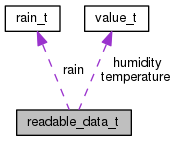
\includegraphics[width=204pt]{structreadable__data__t__coll__graph}
\end{center}
\end{figure}
\subsection*{Public Attributes}
\begin{DoxyCompactItemize}
\item 
\mbox{\Hypertarget{structreadable__data__t_a650c71ad521e965abe34eafda7cf872d}\label{structreadable__data__t_a650c71ad521e965abe34eafda7cf872d}} 
uint8\+\_\+t \hyperlink{structreadable__data__t_a650c71ad521e965abe34eafda7cf872d}{module\+\_\+type}
\begin{DoxyCompactList}\small\item\em module version \end{DoxyCompactList}\item 
\mbox{\Hypertarget{structreadable__data__t_a0b5fa5d2d89bef1b53036512525127f0}\label{structreadable__data__t_a0b5fa5d2d89bef1b53036512525127f0}} 
uint8\+\_\+t \hyperlink{structreadable__data__t_a0b5fa5d2d89bef1b53036512525127f0}{module\+\_\+version}
\begin{DoxyCompactList}\small\item\em module type \end{DoxyCompactList}\item 
\mbox{\Hypertarget{structreadable__data__t_a183ab6eb973fe8deb1c6d0583a991e92}\label{structreadable__data__t_a183ab6eb973fe8deb1c6d0583a991e92}} 
\hyperlink{structrain__t}{rain\+\_\+t} \hyperlink{structreadable__data__t_a183ab6eb973fe8deb1c6d0583a991e92}{rain}
\begin{DoxyCompactList}\small\item\em rain data \end{DoxyCompactList}\item 
\mbox{\Hypertarget{structreadable__data__t_a5852a1cd826e865b18a07fa4be784c6d}\label{structreadable__data__t_a5852a1cd826e865b18a07fa4be784c6d}} 
\hyperlink{structvalue__t}{value\+\_\+t} \hyperlink{structreadable__data__t_a5852a1cd826e865b18a07fa4be784c6d}{temperature}
\begin{DoxyCompactList}\small\item\em temperature data for report \end{DoxyCompactList}\item 
\mbox{\Hypertarget{structreadable__data__t_ab296c803ef271e46364679c955711e26}\label{structreadable__data__t_ab296c803ef271e46364679c955711e26}} 
\hyperlink{structvalue__t}{value\+\_\+t} \hyperlink{structreadable__data__t_ab296c803ef271e46364679c955711e26}{humidity}
\begin{DoxyCompactList}\small\item\em humidity data for report \end{DoxyCompactList}\end{DoxyCompactItemize}


\subsection{Detailed Description}
Readable data through i2c bus. 

The documentation for this struct was generated from the following files\+:\begin{DoxyCompactItemize}
\item 
sketchbook/rmap/i2c-\/rain/\hyperlink{i2c-rain_8h}{i2c-\/rain.\+h}\item 
sketchbook/rmap/i2c-\/th/\hyperlink{i2c-th_8h}{i2c-\/th.\+h}\end{DoxyCompactItemize}

\hypertarget{structsample__t}{}\section{sample\+\_\+t Struct Reference}
\label{structsample__t}\index{sample\+\_\+t@{sample\+\_\+t}}


Samples values for measured temperature and humidity.  




{\ttfamily \#include $<$i2c-\/th.\+h$>$}

\subsection*{Public Attributes}
\begin{DoxyCompactItemize}
\item 
\mbox{\Hypertarget{structsample__t_ab732cec6be98318b8f13563577f7d528}\label{structsample__t_ab732cec6be98318b8f13563577f7d528}} 
uint16\+\_\+t \hyperlink{structsample__t_ab732cec6be98318b8f13563577f7d528}{values} \mbox{[}\hyperlink{i2c-th-config_8h_a5500c7c28f9fc2cab4deffbe07c98b39}{S\+E\+N\+S\+O\+R\+S\+\_\+\+S\+A\+M\+P\+L\+E\+\_\+\+C\+O\+U\+N\+T\+\_\+\+M\+AX}\mbox{]}
\begin{DoxyCompactList}\small\item\em buffer containing the measured samples \end{DoxyCompactList}\item 
\mbox{\Hypertarget{structsample__t_a5a28abacf173c495a32a6f727e5d016e}\label{structsample__t_a5a28abacf173c495a32a6f727e5d016e}} 
uint8\+\_\+t \hyperlink{structsample__t_a5a28abacf173c495a32a6f727e5d016e}{count}
\begin{DoxyCompactList}\small\item\em number of correct samples \end{DoxyCompactList}\item 
\mbox{\Hypertarget{structsample__t_abcd5ae40e49c9c7bbfed40552ba44e72}\label{structsample__t_abcd5ae40e49c9c7bbfed40552ba44e72}} 
uint8\+\_\+t \hyperlink{structsample__t_abcd5ae40e49c9c7bbfed40552ba44e72}{error\+\_\+count}
\begin{DoxyCompactList}\small\item\em number of wrong samples \end{DoxyCompactList}\end{DoxyCompactItemize}


\subsection{Detailed Description}
Samples values for measured temperature and humidity. 

The documentation for this struct was generated from the following file\+:\begin{DoxyCompactItemize}
\item 
sketchbook/rmap/i2c-\/th/\hyperlink{i2c-th_8h}{i2c-\/th.\+h}\end{DoxyCompactItemize}

\hypertarget{structwritable__data__t}{}\section{writable\+\_\+data\+\_\+t Struct Reference}
\label{structwritable__data__t}\index{writable\+\_\+data\+\_\+t@{writable\+\_\+data\+\_\+t}}


Writable data through i2c bus.  




{\ttfamily \#include $<$i2c-\/th.\+h$>$}

\subsection*{Public Attributes}
\begin{DoxyCompactItemize}
\item 
\mbox{\Hypertarget{structwritable__data__t_a539304e9f0f30b03691af8b1e8cb6a16}\label{structwritable__data__t_a539304e9f0f30b03691af8b1e8cb6a16}} 
uint8\+\_\+t \hyperlink{structwritable__data__t_a539304e9f0f30b03691af8b1e8cb6a16}{i2c\+\_\+address}
\begin{DoxyCompactList}\small\item\em i2c address \end{DoxyCompactList}\item 
\mbox{\Hypertarget{structwritable__data__t_afc3c86659df5f3a0840313702c7f66fe}\label{structwritable__data__t_afc3c86659df5f3a0840313702c7f66fe}} 
bool \hyperlink{structwritable__data__t_afc3c86659df5f3a0840313702c7f66fe}{is\+\_\+oneshot}
\begin{DoxyCompactList}\small\item\em enable or disable oneshot mode \end{DoxyCompactList}\item 
\mbox{\Hypertarget{structwritable__data__t_a9c3b7927d969d6f21fe475fd3d67f485}\label{structwritable__data__t_a9c3b7927d969d6f21fe475fd3d67f485}} 
bool \hyperlink{structwritable__data__t_a9c3b7927d969d6f21fe475fd3d67f485}{is\+\_\+continuous}
\begin{DoxyCompactList}\small\item\em enable or disable continuous mode \end{DoxyCompactList}\item 
\mbox{\Hypertarget{structwritable__data__t_ad1852e6418870b503cc307a106aff52e}\label{structwritable__data__t_ad1852e6418870b503cc307a106aff52e}} 
uint8\+\_\+t \hyperlink{structwritable__data__t_ad1852e6418870b503cc307a106aff52e}{i2c\+\_\+temperature\+\_\+address}
\begin{DoxyCompactList}\small\item\em i2c address of temperature sensor \end{DoxyCompactList}\item 
\mbox{\Hypertarget{structwritable__data__t_af7dee4cff91376d89745a86ba747c35f}\label{structwritable__data__t_af7dee4cff91376d89745a86ba747c35f}} 
uint8\+\_\+t \hyperlink{structwritable__data__t_af7dee4cff91376d89745a86ba747c35f}{i2c\+\_\+humidity\+\_\+address}
\begin{DoxyCompactList}\small\item\em i2c address of humidity sensor \end{DoxyCompactList}\end{DoxyCompactItemize}


\subsection{Detailed Description}
Writable data through i2c bus. 

The documentation for this struct was generated from the following file\+:\begin{DoxyCompactItemize}
\item 
\hyperlink{i2c-th_8h}{i2c-\/th.\+h}\end{DoxyCompactItemize}

\chapter{File Documentation}
\hypertarget{i2c-th-config_8h}{}\section{sketchbook/rmap/i2c-\/th/i2c-\/th-\/config.h File Reference}
\label{i2c-th-config_8h}\index{sketchbook/rmap/i2c-\/th/i2c-\/th-\/config.\+h@{sketchbook/rmap/i2c-\/th/i2c-\/th-\/config.\+h}}
{\ttfamily \#include $<$sensors\+\_\+config.\+h$>$}\newline
Include dependency graph for i2c-\/th-\/config.h\+:\nopagebreak
\begin{figure}[H]
\begin{center}
\leavevmode
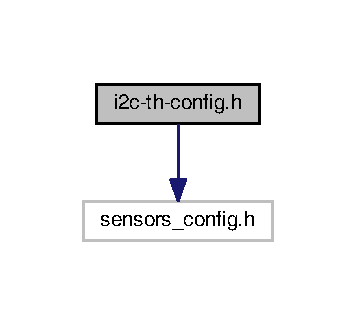
\includegraphics[width=187pt]{i2c-th-config_8h__incl}
\end{center}
\end{figure}
This graph shows which files directly or indirectly include this file\+:\nopagebreak
\begin{figure}[H]
\begin{center}
\leavevmode
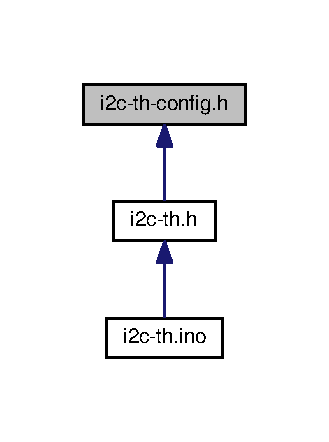
\includegraphics[width=187pt]{i2c-th-config_8h__dep__incl}
\end{center}
\end{figure}
\subsection*{Macros}
\begin{DoxyCompactItemize}
\item 
\mbox{\Hypertarget{i2c-th-config_8h_aa8639a8d4e83d9cc4187d7a751228464}\label{i2c-th-config_8h_aa8639a8d4e83d9cc4187d7a751228464}} 
\#define \hyperlink{i2c-th-config_8h_aa8639a8d4e83d9cc4187d7a751228464}{M\+O\+D\+U\+L\+E\+\_\+\+V\+E\+R\+S\+I\+ON}~(3)
\begin{DoxyCompactList}\small\item\em Module version. \end{DoxyCompactList}\item 
\mbox{\Hypertarget{i2c-th-config_8h_a8c815d03b3fd3e18ca06f920a1eb4e8e}\label{i2c-th-config_8h_a8c815d03b3fd3e18ca06f920a1eb4e8e}} 
\#define \hyperlink{i2c-th-config_8h_a8c815d03b3fd3e18ca06f920a1eb4e8e}{M\+O\+D\+U\+L\+E\+\_\+\+T\+Y\+PE}~(\hyperlink{stima__module_8h_ab4d075291417ea1254b52a2db807c89d}{S\+T\+I\+M\+A\+\_\+\+M\+O\+D\+U\+L\+E\+\_\+\+T\+Y\+P\+E\+\_\+\+TH})
\begin{DoxyCompactList}\small\item\em Type of module. It is defined in \hyperlink{registers_8h}{registers.\+h}. \end{DoxyCompactList}\item 
\mbox{\Hypertarget{i2c-th-config_8h_a5c4024778a87026713c77babd50c06e8}\label{i2c-th-config_8h_a5c4024778a87026713c77babd50c06e8}} 
\#define \hyperlink{i2c-th-config_8h_a5c4024778a87026713c77babd50c06e8}{C\+O\+N\+F\+I\+G\+U\+R\+A\+T\+I\+O\+N\+\_\+\+D\+E\+F\+A\+U\+L\+T\+\_\+\+I\+S\+\_\+\+O\+N\+E\+S\+H\+OT}~(false)
\begin{DoxyCompactList}\small\item\em Oneshot mode for default. \end{DoxyCompactList}\item 
\mbox{\Hypertarget{i2c-th-config_8h_a21819dc42c8c71731e30c99bcf8b0f76}\label{i2c-th-config_8h_a21819dc42c8c71731e30c99bcf8b0f76}} 
\#define \hyperlink{i2c-th-config_8h_a21819dc42c8c71731e30c99bcf8b0f76}{C\+O\+N\+F\+I\+G\+U\+R\+A\+T\+I\+O\+N\+\_\+\+D\+E\+F\+A\+U\+L\+T\+\_\+\+I\+S\+\_\+\+C\+O\+N\+T\+I\+N\+U\+O\+US}~(true)
\begin{DoxyCompactList}\small\item\em Continuous mode for default. \end{DoxyCompactList}\item 
\mbox{\Hypertarget{i2c-th-config_8h_a25fb304ef264a84353f1d4cfc61128e9}\label{i2c-th-config_8h_a25fb304ef264a84353f1d4cfc61128e9}} 
\#define \hyperlink{i2c-th-config_8h_a25fb304ef264a84353f1d4cfc61128e9}{C\+O\+N\+F\+I\+G\+U\+R\+A\+T\+I\+O\+N\+\_\+\+D\+E\+F\+A\+U\+L\+T\+\_\+\+I2\+C\+\_\+\+A\+D\+D\+R\+E\+SS}~(\hyperlink{registers-th_8h_a66906eb81e92beab5f2076ac49996132}{I2\+C\+\_\+\+T\+H\+\_\+\+D\+E\+F\+A\+U\+L\+T\+\_\+\+A\+D\+D\+R\+E\+SS})
\begin{DoxyCompactList}\small\item\em Default i2c address. \end{DoxyCompactList}\item 
\mbox{\Hypertarget{i2c-th-config_8h_afd732a8bd16aa3939928851656adb365}\label{i2c-th-config_8h_afd732a8bd16aa3939928851656adb365}} 
\#define \hyperlink{i2c-th-config_8h_afd732a8bd16aa3939928851656adb365}{C\+O\+N\+F\+I\+G\+U\+R\+A\+T\+I\+O\+N\+\_\+\+D\+E\+F\+A\+U\+L\+T\+\_\+\+T\+E\+M\+P\+E\+R\+A\+T\+U\+R\+E\+\_\+\+A\+D\+D\+R\+E\+SS}~(\hyperlink{registers-th_8h_a6d2d1a9b4ae7894be4b062205255f1ff}{I2\+C\+\_\+\+T\+H\+\_\+\+T\+E\+M\+P\+E\+R\+A\+T\+U\+R\+E\+\_\+\+D\+E\+F\+A\+U\+L\+T\+\_\+\+A\+D\+D\+R\+E\+SS})
\begin{DoxyCompactList}\small\item\em Default i2c temperature address. \end{DoxyCompactList}\item 
\mbox{\Hypertarget{i2c-th-config_8h_a6d8fda545e952788d1692c9395b2ff2d}\label{i2c-th-config_8h_a6d8fda545e952788d1692c9395b2ff2d}} 
\#define \hyperlink{i2c-th-config_8h_a6d8fda545e952788d1692c9395b2ff2d}{C\+O\+N\+F\+I\+G\+U\+R\+A\+T\+I\+O\+N\+\_\+\+D\+E\+F\+A\+U\+L\+T\+\_\+\+H\+U\+M\+I\+D\+I\+T\+Y\+\_\+\+A\+D\+D\+R\+E\+SS}~(\hyperlink{registers-th_8h_aa7b1a0982e4333dd39c7829eda6baa42}{I2\+C\+\_\+\+T\+H\+\_\+\+H\+U\+M\+I\+D\+I\+T\+Y\+\_\+\+D\+E\+F\+A\+U\+L\+T\+\_\+\+A\+D\+D\+R\+E\+SS})
\begin{DoxyCompactList}\small\item\em Default i2c humidity address. \end{DoxyCompactList}\item 
\mbox{\Hypertarget{i2c-th-config_8h_ae90da4786d4ba14563681879dba4d39c}\label{i2c-th-config_8h_ae90da4786d4ba14563681879dba4d39c}} 
\#define \hyperlink{i2c-th-config_8h_ae90da4786d4ba14563681879dba4d39c}{C\+O\+N\+F\+I\+G\+U\+R\+A\+T\+I\+O\+N\+\_\+\+R\+E\+S\+E\+T\+\_\+\+P\+IN}~(8)
\begin{DoxyCompactList}\small\item\em Input pin for reset configuration at startup. \end{DoxyCompactList}\item 
\mbox{\Hypertarget{i2c-th-config_8h_a9ace81994cbeb6153f9dd5adf0e6dbee}\label{i2c-th-config_8h_a9ace81994cbeb6153f9dd5adf0e6dbee}} 
\#define \hyperlink{i2c-th-config_8h_a9ace81994cbeb6153f9dd5adf0e6dbee}{U\+S\+E\+\_\+\+P\+O\+W\+E\+R\+\_\+\+D\+O\+WN}~(true)
\begin{DoxyCompactList}\small\item\em Enable or disable power down. \end{DoxyCompactList}\item 
\mbox{\Hypertarget{i2c-th-config_8h_a7b9497e328b8f872cd7677cfd02bbf65}\label{i2c-th-config_8h_a7b9497e328b8f872cd7677cfd02bbf65}} 
\#define \hyperlink{i2c-th-config_8h_a7b9497e328b8f872cd7677cfd02bbf65}{D\+E\+B\+O\+U\+N\+C\+I\+N\+G\+\_\+\+P\+O\+W\+E\+R\+\_\+\+D\+O\+W\+N\+\_\+\+T\+I\+M\+E\+\_\+\+MS}~(10)
\begin{DoxyCompactList}\small\item\em Debounce power down ms. \end{DoxyCompactList}\item 
\mbox{\Hypertarget{i2c-th-config_8h_a8051c2a569a9f9c488af89bce47ec306}\label{i2c-th-config_8h_a8051c2a569a9f9c488af89bce47ec306}} 
\#define \hyperlink{i2c-th-config_8h_a8051c2a569a9f9c488af89bce47ec306}{U\+S\+E\+\_\+\+T\+I\+M\+E\+R\+\_\+1}~(true)
\begin{DoxyCompactList}\small\item\em Enable or disable timer1. \end{DoxyCompactList}\item 
\#define \hyperlink{i2c-th-config_8h_a983c9777673ee873f12ec9f489215321}{W\+D\+T\+\_\+\+T\+I\+M\+ER}~(W\+D\+T\+O\+\_\+8S)
\begin{DoxyCompactList}\small\item\em Watchdog timer for periodically check microprocessor block states. \end{DoxyCompactList}\item 
\mbox{\Hypertarget{i2c-th-config_8h_a94909b75c6bbb3614c483f1d22462440}\label{i2c-th-config_8h_a94909b75c6bbb3614c483f1d22462440}} 
\#define \hyperlink{i2c-th-config_8h_a94909b75c6bbb3614c483f1d22462440}{S\+E\+N\+S\+O\+R\+S\+\_\+\+S\+A\+M\+P\+L\+E\+\_\+\+T\+I\+M\+E\+\_\+\+MS}~(4000)
\begin{DoxyCompactList}\small\item\em Milliseconds for sampling sensors\+: 2000 -\/ 8000 \mbox{[}ms\mbox{]}. \end{DoxyCompactList}\item 
\mbox{\Hypertarget{i2c-th-config_8h_a05567a696548b4a2e03c49dc893a32c8}\label{i2c-th-config_8h_a05567a696548b4a2e03c49dc893a32c8}} 
\#define \hyperlink{i2c-th-config_8h_a05567a696548b4a2e03c49dc893a32c8}{S\+E\+N\+S\+O\+R\+S\+\_\+\+S\+A\+M\+P\+L\+E\+\_\+\+C\+O\+U\+N\+T\+\_\+\+M\+IN}~((uint8\+\_\+t)(\hyperlink{sensors__config_8h_acd6a77ef70e6cd768267a4e3d79cf981}{O\+B\+S\+E\+R\+V\+A\+T\+I\+O\+N\+S\+\_\+\+M\+I\+N\+U\+T\+ES} $\ast$ 60 / ((uint8\+\_\+t)(\hyperlink{i2c-th-config_8h_a94909b75c6bbb3614c483f1d22462440}{S\+E\+N\+S\+O\+R\+S\+\_\+\+S\+A\+M\+P\+L\+E\+\_\+\+T\+I\+M\+E\+\_\+\+MS} / 1000))))
\begin{DoxyCompactList}\small\item\em Sample count minimum in O\+B\+S\+E\+R\+V\+A\+T\+I\+O\+N\+S\+\_\+\+M\+I\+N\+U\+T\+ES minutes. \end{DoxyCompactList}\item 
\mbox{\Hypertarget{i2c-th-config_8h_a5500c7c28f9fc2cab4deffbe07c98b39}\label{i2c-th-config_8h_a5500c7c28f9fc2cab4deffbe07c98b39}} 
\#define \hyperlink{i2c-th-config_8h_a5500c7c28f9fc2cab4deffbe07c98b39}{S\+E\+N\+S\+O\+R\+S\+\_\+\+S\+A\+M\+P\+L\+E\+\_\+\+C\+O\+U\+N\+T\+\_\+\+M\+AX}~(\hyperlink{i2c-th-config_8h_a05567a696548b4a2e03c49dc893a32c8}{S\+E\+N\+S\+O\+R\+S\+\_\+\+S\+A\+M\+P\+L\+E\+\_\+\+C\+O\+U\+N\+T\+\_\+\+M\+IN})
\begin{DoxyCompactList}\small\item\em Sample count maximum in O\+B\+S\+E\+R\+V\+A\+T\+I\+O\+N\+S\+\_\+\+M\+I\+N\+U\+T\+ES minutes. \end{DoxyCompactList}\item 
\mbox{\Hypertarget{i2c-th-config_8h_a4ee69ccbdc607eb03834e7cf1d950ec0}\label{i2c-th-config_8h_a4ee69ccbdc607eb03834e7cf1d950ec0}} 
\#define \hyperlink{i2c-th-config_8h_a4ee69ccbdc607eb03834e7cf1d950ec0}{S\+E\+N\+S\+O\+R\+S\+\_\+\+S\+A\+M\+P\+L\+E\+\_\+\+C\+O\+U\+N\+T\+\_\+\+T\+O\+L\+E\+R\+A\+N\+CE}~(2)
\begin{DoxyCompactList}\small\item\em Maximum invalid sample count for generate a valid observations. \end{DoxyCompactList}\item 
\mbox{\Hypertarget{i2c-th-config_8h_af18dc3de744722cb308451b7a705611b}\label{i2c-th-config_8h_af18dc3de744722cb308451b7a705611b}} 
\#define \hyperlink{i2c-th-config_8h_af18dc3de744722cb308451b7a705611b}{U\+S\+E\+\_\+\+S\+E\+N\+S\+O\+R\+S\+\_\+\+C\+O\+U\+NT}~(\hyperlink{sensors__config_8h_a34acfad25488d28951ff729ebda66311}{U\+S\+E\+\_\+\+S\+E\+N\+S\+O\+R\+\_\+\+A\+DT} + \hyperlink{sensors__config_8h_aa1d83db2373ab5e74ed832abf1b7f0ed}{U\+S\+E\+\_\+\+S\+E\+N\+S\+O\+R\+\_\+\+H\+IH} + \hyperlink{sensors__config_8h_a85f2976107ff26789b268febf87a392a}{U\+S\+E\+\_\+\+S\+E\+N\+S\+O\+R\+\_\+\+H\+YT})
\begin{DoxyCompactList}\small\item\em Sensors count. \end{DoxyCompactList}\item 
\mbox{\Hypertarget{i2c-th-config_8h_a42354f9347cc2a67e00dd79c5da40833}\label{i2c-th-config_8h_a42354f9347cc2a67e00dd79c5da40833}} 
\#define \hyperlink{i2c-th-config_8h_a42354f9347cc2a67e00dd79c5da40833}{T\+I\+M\+E\+R1\+\_\+\+I\+N\+T\+E\+R\+R\+U\+P\+T\+\_\+\+T\+I\+M\+E\+\_\+\+MS}~(4000)
\begin{DoxyCompactList}\small\item\em Value in milliseconds for generating timer1 interrupt. \end{DoxyCompactList}\item 
\mbox{\Hypertarget{i2c-th-config_8h_aa4674bad300dfeeb4b9479c5bdc21036}\label{i2c-th-config_8h_aa4674bad300dfeeb4b9479c5bdc21036}} 
\#define \hyperlink{i2c-th-config_8h_aa4674bad300dfeeb4b9479c5bdc21036}{T\+I\+M\+E\+R1\+\_\+\+O\+V\+E\+R\+F\+L\+O\+W\+\_\+\+T\+I\+M\+E\+\_\+\+MS}~(8388)
\begin{DoxyCompactList}\small\item\em Timer1 timer overflow with 1024 prescaler at 8 M\+Hz. \end{DoxyCompactList}\item 
\mbox{\Hypertarget{i2c-th-config_8h_a346c738fa798abcc0c070d068da6380f}\label{i2c-th-config_8h_a346c738fa798abcc0c070d068da6380f}} 
\#define \hyperlink{i2c-th-config_8h_a346c738fa798abcc0c070d068da6380f}{T\+I\+M\+E\+R1\+\_\+\+T\+C\+N\+T1\+\_\+\+V\+A\+L\+UE}~((uint16\+\_\+t)(0x\+F\+F\+F\+F -\/ (float)(1.\+0 $\ast$ 0x\+F\+F\+F\+F $\ast$ T\+I\+M\+E\+R1\+\_\+\+I\+N\+T\+E\+R\+R\+U\+P\+T\+\_\+\+T\+I\+M\+E\+\_\+\+M\+S / T\+I\+M\+E\+R1\+\_\+\+O\+V\+E\+R\+F\+L\+O\+W\+\_\+\+T\+I\+M\+E\+\_\+\+M\+S)))
\begin{DoxyCompactList}\small\item\em Timer1 timer overflow with 1024 prescaler at 8 M\+Hz. \end{DoxyCompactList}\item 
\mbox{\Hypertarget{i2c-th-config_8h_a988c83777a3764544137ac7493c3d0ac}\label{i2c-th-config_8h_a988c83777a3764544137ac7493c3d0ac}} 
\#define \hyperlink{i2c-th-config_8h_a988c83777a3764544137ac7493c3d0ac}{T\+I\+M\+E\+R1\+\_\+\+V\+A\+L\+U\+E\+\_\+\+M\+A\+X\+\_\+\+MS}~(12000)
\begin{DoxyCompactList}\small\item\em Maximum timer1 counter value for timed tasks. \end{DoxyCompactList}\item 
\mbox{\Hypertarget{i2c-th-config_8h_a16fa5577ef44bb1146f17a3bc43194b1}\label{i2c-th-config_8h_a16fa5577ef44bb1146f17a3bc43194b1}} 
\#define \hyperlink{i2c-th-config_8h_a16fa5577ef44bb1146f17a3bc43194b1}{S\+E\+N\+S\+O\+R\+S\+\_\+\+R\+E\+T\+R\+Y\+\_\+\+C\+O\+U\+N\+T\+\_\+\+M\+AX}~(3)
\begin{DoxyCompactList}\small\item\em Maximum number of retry for sensors reading. \end{DoxyCompactList}\item 
\mbox{\Hypertarget{i2c-th-config_8h_a8ea8eeea7855628652f697bab3d173b5}\label{i2c-th-config_8h_a8ea8eeea7855628652f697bab3d173b5}} 
\#define \hyperlink{i2c-th-config_8h_a8ea8eeea7855628652f697bab3d173b5}{S\+E\+N\+S\+O\+R\+S\+\_\+\+R\+E\+T\+R\+Y\+\_\+\+D\+E\+L\+A\+Y\+\_\+\+MS}~(50)
\begin{DoxyCompactList}\small\item\em Waiting for reading between two attempts. \end{DoxyCompactList}\end{DoxyCompactItemize}


\subsection{Macro Definition Documentation}
\mbox{\Hypertarget{i2c-th-config_8h_a983c9777673ee873f12ec9f489215321}\label{i2c-th-config_8h_a983c9777673ee873f12ec9f489215321}} 
\index{i2c-\/th-\/config.\+h@{i2c-\/th-\/config.\+h}!W\+D\+T\+\_\+\+T\+I\+M\+ER@{W\+D\+T\+\_\+\+T\+I\+M\+ER}}
\index{W\+D\+T\+\_\+\+T\+I\+M\+ER@{W\+D\+T\+\_\+\+T\+I\+M\+ER}!i2c-\/th-\/config.\+h@{i2c-\/th-\/config.\+h}}
\subsubsection{\texorpdfstring{W\+D\+T\+\_\+\+T\+I\+M\+ER}{WDT\_TIMER}}
{\footnotesize\ttfamily \#define W\+D\+T\+\_\+\+T\+I\+M\+ER~(W\+D\+T\+O\+\_\+8S)}



Watchdog timer for periodically check microprocessor block states. 

Possible value for W\+D\+T\+\_\+\+T\+I\+M\+ER are\+: W\+D\+T\+O\+\_\+15\+MS, W\+D\+T\+O\+\_\+30\+MS, W\+D\+T\+O\+\_\+60\+MS, W\+D\+T\+O\+\_\+120\+MS, W\+D\+T\+O\+\_\+250\+MS, W\+D\+T\+O\+\_\+500\+MS, W\+D\+T\+O\+\_\+1S, W\+D\+T\+O\+\_\+2S, W\+D\+T\+O\+\_\+4S, W\+D\+T\+O\+\_\+8S 
\hypertarget{i2c-th_8h}{}\section{sketchbook/rmap/i2c-\/th/i2c-\/th.h File Reference}
\label{i2c-th_8h}\index{sketchbook/rmap/i2c-\/th/i2c-\/th.\+h@{sketchbook/rmap/i2c-\/th/i2c-\/th.\+h}}
{\ttfamily \#include \char`\"{}i2c-\/th-\/config.\+h\char`\"{}}\newline
{\ttfamily \#include $<$debug.\+h$>$}\newline
{\ttfamily \#include $<$hardware\+\_\+config.\+h$>$}\newline
{\ttfamily \#include $<$avr/sleep.\+h$>$}\newline
{\ttfamily \#include $<$avr/power.\+h$>$}\newline
{\ttfamily \#include $<$avr/wdt.\+h$>$}\newline
{\ttfamily \#include $<$i2c\+\_\+utility.\+h$>$}\newline
{\ttfamily \#include $<$rmap\+\_\+utility.\+h$>$}\newline
{\ttfamily \#include $<$eeprom\+\_\+utility.\+h$>$}\newline
{\ttfamily \#include $<$Wire.\+h$>$}\newline
{\ttfamily \#include $<$Time\+Lib.\+h$>$}\newline
{\ttfamily \#include $<$typedef.\+h$>$}\newline
{\ttfamily \#include $<$registers-\/th.\+h$>$}\newline
{\ttfamily \#include $<$Sensor\+Driver.\+h$>$}\newline
Include dependency graph for i2c-\/th.h\+:
\nopagebreak
\begin{figure}[H]
\begin{center}
\leavevmode
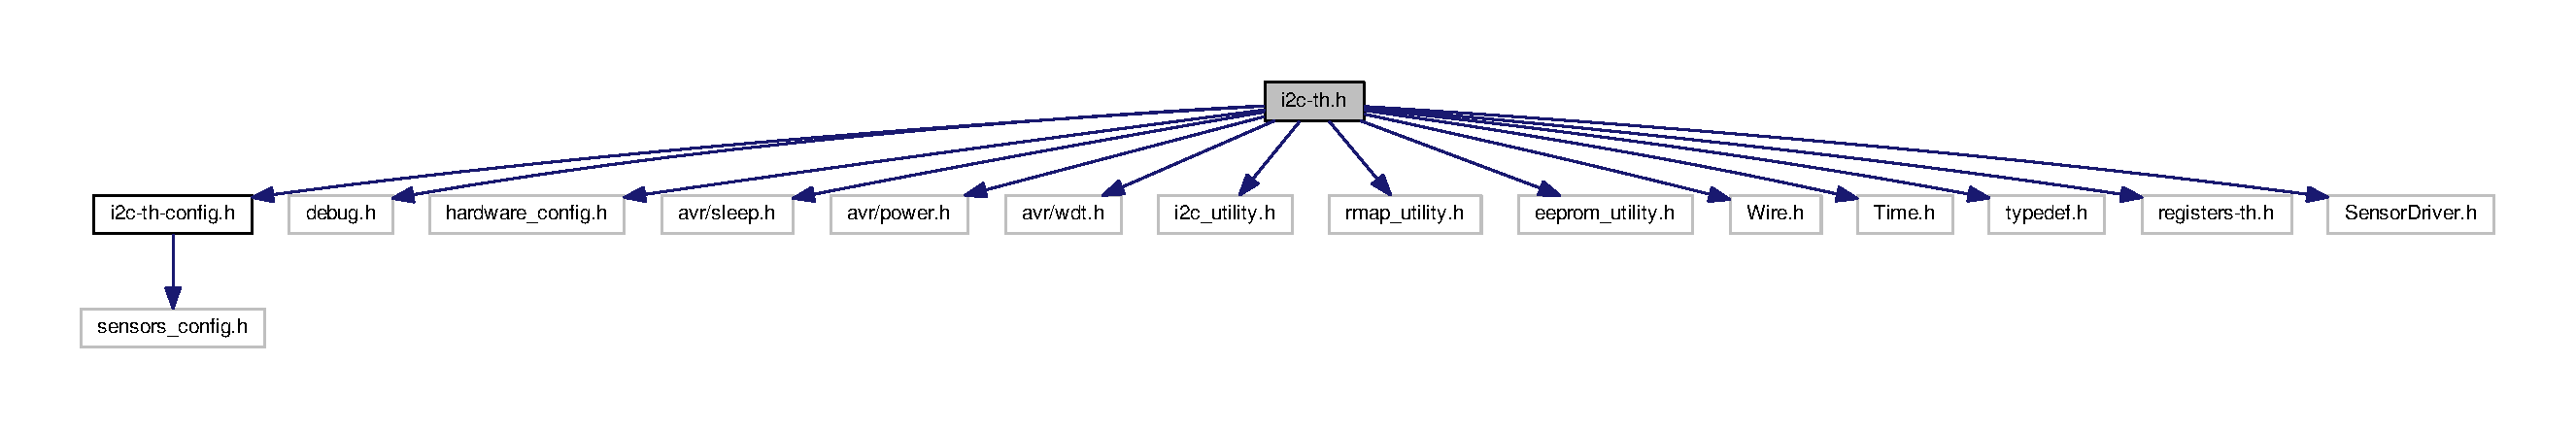
\includegraphics[width=350pt]{i2c-th_8h__incl}
\end{center}
\end{figure}
This graph shows which files directly or indirectly include this file\+:
\nopagebreak
\begin{figure}[H]
\begin{center}
\leavevmode
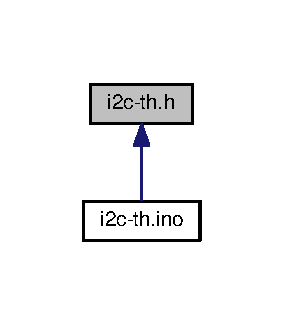
\includegraphics[width=187pt]{i2c-th_8h__dep__incl}
\end{center}
\end{figure}
\subsection*{Classes}
\begin{DoxyCompactItemize}
\item 
struct \hyperlink{structconfiguration__t}{configuration\+\_\+t}
\begin{DoxyCompactList}\small\item\em E\+E\+P\+R\+OM saved configuration. \end{DoxyCompactList}\item 
struct \hyperlink{structreadable__data__t}{readable\+\_\+data\+\_\+t}
\begin{DoxyCompactList}\small\item\em Readable data through i2c bus. \end{DoxyCompactList}\item 
struct \hyperlink{structwritable__data__t}{writable\+\_\+data\+\_\+t}
\begin{DoxyCompactList}\small\item\em Writable data through i2c bus. \end{DoxyCompactList}\item 
struct \hyperlink{structsample__t}{sample\+\_\+t}
\begin{DoxyCompactList}\small\item\em Samples values for measured temperature and humidity. \end{DoxyCompactList}\item 
struct \hyperlink{structobservation__t}{observation\+\_\+t}
\begin{DoxyCompactList}\small\item\em Observations values for temperature and humidity. \end{DoxyCompactList}\end{DoxyCompactItemize}
\subsection*{Enumerations}
\begin{DoxyCompactItemize}
\item 
enum \hyperlink{i2c-th_8h_aa0aafed44fec19806d8f9ad834be1248}{state\+\_\+t} \{ \newline
\hyperlink{i2c-rain_8h_aa0aafed44fec19806d8f9ad834be1248a0cb1b2c6a7db1f1084886c98909a3f36}{I\+N\+IT}, 
\hyperlink{i2c-rain_8h_aa0aafed44fec19806d8f9ad834be1248a34f1df650a5075369a6827770c433a91}{T\+A\+S\+K\+S\+\_\+\+E\+X\+E\+C\+U\+T\+I\+ON}, 
\hyperlink{i2c-rain_8h_aa0aafed44fec19806d8f9ad834be1248adc6f24fd6915a3f2786a1b7045406924}{E\+ND}, 
\hyperlink{i2c-th_8h_aa0aafed44fec19806d8f9ad834be1248a0cb1b2c6a7db1f1084886c98909a3f36}{I\+N\+IT}, 
\newline
\hyperlink{i2c-th_8h_aa0aafed44fec19806d8f9ad834be1248a34f1df650a5075369a6827770c433a91}{T\+A\+S\+K\+S\+\_\+\+E\+X\+E\+C\+U\+T\+I\+ON}, 
\hyperlink{i2c-th_8h_aa0aafed44fec19806d8f9ad834be1248adc6f24fd6915a3f2786a1b7045406924}{E\+ND}, 
\hyperlink{rmap_8h_aa0aafed44fec19806d8f9ad834be1248a0cb1b2c6a7db1f1084886c98909a3f36}{I\+N\+IT}, 
\hyperlink{rmap_8h_aa0aafed44fec19806d8f9ad834be1248a34f1df650a5075369a6827770c433a91}{T\+A\+S\+K\+S\+\_\+\+E\+X\+E\+C\+U\+T\+I\+ON}, 
\newline
\hyperlink{rmap_8h_aa0aafed44fec19806d8f9ad834be1248adc6f24fd6915a3f2786a1b7045406924}{E\+ND}
 \}
\item 
enum \hyperlink{i2c-th_8h_a48bef3d022ff6f88967496ad53a6b953}{sensors\+\_\+reading\+\_\+state\+\_\+t} \{ \newline
\hyperlink{i2c-th_8h_a48bef3d022ff6f88967496ad53a6b953a2cb28b4d2ce509fc382d6bd1b2d5d16f}{S\+E\+N\+S\+O\+R\+S\+\_\+\+R\+E\+A\+D\+I\+N\+G\+\_\+\+I\+N\+IT}, 
\hyperlink{i2c-th_8h_a48bef3d022ff6f88967496ad53a6b953a7cf0f5ecc300e86aacc2deb266d14724}{S\+E\+N\+S\+O\+R\+S\+\_\+\+R\+E\+A\+D\+I\+N\+G\+\_\+\+P\+R\+E\+P\+A\+RE}, 
\hyperlink{i2c-th_8h_a48bef3d022ff6f88967496ad53a6b953a96e335eefffa76f53459df4a3cf71ac1}{S\+E\+N\+S\+O\+R\+S\+\_\+\+R\+E\+A\+D\+I\+N\+G\+\_\+\+I\+S\+\_\+\+P\+R\+E\+P\+A\+R\+ED}, 
\hyperlink{i2c-th_8h_a48bef3d022ff6f88967496ad53a6b953a8e031386ec7bcc225e75a4a0b408d731}{S\+E\+N\+S\+O\+R\+S\+\_\+\+R\+E\+A\+D\+I\+N\+G\+\_\+\+G\+ET}, 
\newline
\hyperlink{i2c-th_8h_a48bef3d022ff6f88967496ad53a6b953a3dae8abf31ae3db2ab2d679c224fd8be}{S\+E\+N\+S\+O\+R\+S\+\_\+\+R\+E\+A\+D\+I\+N\+G\+\_\+\+I\+S\+\_\+\+G\+E\+T\+T\+ED}, 
\hyperlink{i2c-th_8h_a48bef3d022ff6f88967496ad53a6b953ac2ebb8ebf9d29905d0a30f804376b9fa}{S\+E\+N\+S\+O\+R\+S\+\_\+\+R\+E\+A\+D\+I\+N\+G\+\_\+\+R\+E\+AD}, 
\hyperlink{i2c-th_8h_a48bef3d022ff6f88967496ad53a6b953a739c69b8d018187b0956660ed209e303}{S\+E\+N\+S\+O\+R\+S\+\_\+\+R\+E\+A\+D\+I\+N\+G\+\_\+\+N\+E\+XT}, 
\hyperlink{i2c-th_8h_a48bef3d022ff6f88967496ad53a6b953ab602220e588f3c2ac15b450239d9577a}{S\+E\+N\+S\+O\+R\+S\+\_\+\+R\+E\+A\+D\+I\+N\+G\+\_\+\+E\+ND}, 
\newline
\hyperlink{i2c-th_8h_a48bef3d022ff6f88967496ad53a6b953acfc850b971651f7c8c90cddf593fa399}{S\+E\+N\+S\+O\+R\+S\+\_\+\+R\+E\+A\+D\+I\+N\+G\+\_\+\+W\+A\+I\+T\+\_\+\+S\+T\+A\+TE}, 
\hyperlink{rmap_8h_a48bef3d022ff6f88967496ad53a6b953a2cb28b4d2ce509fc382d6bd1b2d5d16f}{S\+E\+N\+S\+O\+R\+S\+\_\+\+R\+E\+A\+D\+I\+N\+G\+\_\+\+I\+N\+IT}, 
\hyperlink{rmap_8h_a48bef3d022ff6f88967496ad53a6b953a7cf0f5ecc300e86aacc2deb266d14724}{S\+E\+N\+S\+O\+R\+S\+\_\+\+R\+E\+A\+D\+I\+N\+G\+\_\+\+P\+R\+E\+P\+A\+RE}, 
\hyperlink{rmap_8h_a48bef3d022ff6f88967496ad53a6b953a96e335eefffa76f53459df4a3cf71ac1}{S\+E\+N\+S\+O\+R\+S\+\_\+\+R\+E\+A\+D\+I\+N\+G\+\_\+\+I\+S\+\_\+\+P\+R\+E\+P\+A\+R\+ED}, 
\newline
\hyperlink{rmap_8h_a48bef3d022ff6f88967496ad53a6b953a8e031386ec7bcc225e75a4a0b408d731}{S\+E\+N\+S\+O\+R\+S\+\_\+\+R\+E\+A\+D\+I\+N\+G\+\_\+\+G\+ET}, 
\hyperlink{rmap_8h_a48bef3d022ff6f88967496ad53a6b953a3dae8abf31ae3db2ab2d679c224fd8be}{S\+E\+N\+S\+O\+R\+S\+\_\+\+R\+E\+A\+D\+I\+N\+G\+\_\+\+I\+S\+\_\+\+G\+E\+T\+T\+ED}, 
\hyperlink{rmap_8h_a48bef3d022ff6f88967496ad53a6b953ac2ebb8ebf9d29905d0a30f804376b9fa}{S\+E\+N\+S\+O\+R\+S\+\_\+\+R\+E\+A\+D\+I\+N\+G\+\_\+\+R\+E\+AD}, 
\hyperlink{rmap_8h_a48bef3d022ff6f88967496ad53a6b953a739c69b8d018187b0956660ed209e303}{S\+E\+N\+S\+O\+R\+S\+\_\+\+R\+E\+A\+D\+I\+N\+G\+\_\+\+N\+E\+XT}, 
\newline
\hyperlink{rmap_8h_a48bef3d022ff6f88967496ad53a6b953ab602220e588f3c2ac15b450239d9577a}{S\+E\+N\+S\+O\+R\+S\+\_\+\+R\+E\+A\+D\+I\+N\+G\+\_\+\+E\+ND}, 
\hyperlink{rmap_8h_a48bef3d022ff6f88967496ad53a6b953acfc850b971651f7c8c90cddf593fa399}{S\+E\+N\+S\+O\+R\+S\+\_\+\+R\+E\+A\+D\+I\+N\+G\+\_\+\+W\+A\+I\+T\+\_\+\+S\+T\+A\+TE}
 \}\begin{DoxyCompactList}\small\item\em Sensors reading task finite state machine. \end{DoxyCompactList}
\end{DoxyCompactItemize}
\subsection*{Functions}
\begin{DoxyCompactItemize}
\item 
void \hyperlink{i2c-th_8h_afb98a0f07c30784284f48271ffe02b97}{init\+\_\+power\+\_\+down} (uint32\+\_\+t $\ast$time\+\_\+ms, uint32\+\_\+t debouncing\+\_\+ms)
\begin{DoxyCompactList}\small\item\em Enter power down mode. \end{DoxyCompactList}\item 
void \hyperlink{i2c-th_8h_a980e73df66b14b1190bc25da430a4f12}{init\+\_\+wdt} (uint8\+\_\+t wdt\+\_\+timer)
\begin{DoxyCompactList}\small\item\em Init watchdog. \end{DoxyCompactList}\item 
void \hyperlink{i2c-th_8h_a348d23d5899ce59d18975284dfb0afc0}{init\+\_\+system} (void)
\begin{DoxyCompactList}\small\item\em Init system. \end{DoxyCompactList}\item 
void \hyperlink{i2c-th_8h_ad438327c9cf783bd9c519ce8b8ef3bfa}{init\+\_\+buffers} (void)
\begin{DoxyCompactList}\small\item\em Init buffers. \end{DoxyCompactList}\item 
void \hyperlink{i2c-th_8h_a2aae2290a141fddcea3fb6009acbb445}{init\+\_\+tasks} (void)
\begin{DoxyCompactList}\small\item\em Init tasks variable and state. \end{DoxyCompactList}\item 
void \hyperlink{i2c-th_8h_aa9c113540346b54d49b2a596e6ba8480}{init\+\_\+pins} (void)
\begin{DoxyCompactList}\small\item\em Init hardware pins. \end{DoxyCompactList}\item 
void \hyperlink{i2c-th_8h_a7c21452937863fa02a29654247eef09b}{init\+\_\+wire} (void)
\begin{DoxyCompactList}\small\item\em Init wire (i2c) library and performs checks on the bus. \end{DoxyCompactList}\item 
void \hyperlink{i2c-th_8h_a4454f968b2402a0e61deb15ab2571dab}{init\+\_\+spi} (void)
\begin{DoxyCompactList}\small\item\em Init S\+PI library. \end{DoxyCompactList}\item 
void \hyperlink{i2c-th_8h_a88533ad02465ce52d4e6de7b2095ec32}{init\+\_\+rtc} (void)
\begin{DoxyCompactList}\small\item\em Init R\+TC module. \end{DoxyCompactList}\item 
void \hyperlink{i2c-th_8h_ad7577ba7f06f417a019b69da8682ede5}{init\+\_\+sensors} (void)
\begin{DoxyCompactList}\small\item\em Create and setup sensors. \end{DoxyCompactList}\item 
void \hyperlink{i2c-th_8h_ab08b9047f47849f399950705e769be2e}{print\+\_\+configuration} (void)
\begin{DoxyCompactList}\small\item\em Print current configuration. \end{DoxyCompactList}\item 
void \hyperlink{i2c-th_8h_a1be652e7d942160a14a560e0be837358}{load\+\_\+configuration} (void)
\begin{DoxyCompactList}\small\item\em Load configuration from E\+E\+P\+R\+OM. \end{DoxyCompactList}\item 
void \hyperlink{i2c-th_8h_a8801fa7c9f323c5b8b9b2bb5b1c438ff}{save\+\_\+configuration} (bool)
\begin{DoxyCompactList}\small\item\em Save configuration to E\+E\+P\+R\+OM. \end{DoxyCompactList}\item 
void \hyperlink{i2c-th_8h_aaad2f6556489c51f2c24302e2cb4188a}{commands} (void)
\begin{DoxyCompactList}\small\item\em Performs specific operations based on the received command. \end{DoxyCompactList}\item 
void \hyperlink{i2c-th_8h_a5f6b7d25ff64c2ddaa0fadd3058fcee3}{reset\+\_\+samples\+\_\+buffer} (void)
\begin{DoxyCompactList}\small\item\em Reset samples buffers to default value. \end{DoxyCompactList}\item 
void \hyperlink{i2c-th_8h_a49fdbb850fac1a3832e7852a24c31c72}{reset\+\_\+observations\+\_\+buffer} (void)
\begin{DoxyCompactList}\small\item\em Reset observations buffers to default value. \end{DoxyCompactList}\item 
void \hyperlink{i2c-th_8h_aafa3d59a1bde3085849eee08f110612f}{exchange\+\_\+buffers} (void)
\begin{DoxyCompactList}\small\item\em Exchange reader and writer pointer to buffer. \end{DoxyCompactList}\item 
void \hyperlink{i2c-th_8h_aba0fc91d6c2829df00a9d5fe2b921c90}{samples\+\_\+processing} (bool is\+\_\+force\+\_\+processing)
\begin{DoxyCompactList}\small\item\em Main routine for processing the samples to calculate an observation. \end{DoxyCompactList}\item 
void \hyperlink{i2c-th_8h_a8b67eda853f3e8cca0c729267b492861}{observations\+\_\+processing} (void)
\begin{DoxyCompactList}\small\item\em Main routine for processing the observations to calculate a value for report. \end{DoxyCompactList}\item 
bool \hyperlink{i2c-th_8h_a1c5769e114267b210fb3812064d01dd0}{make\+\_\+observation\+\_\+from\+\_\+samples} (bool is\+\_\+force\+\_\+processing, \hyperlink{structsample__t}{sample\+\_\+t} $\ast$sample, \hyperlink{structobservation__t}{observation\+\_\+t} $\ast$observation)
\begin{DoxyCompactList}\small\item\em Processing the samples to calculate an observation when the number of the samples reaches the exact samples\+\_\+count value. \end{DoxyCompactList}\item 
bool \hyperlink{i2c-th_8h_ab301e4d552826ef91458f52963949a1d}{make\+\_\+value\+\_\+from\+\_\+samples\+\_\+and\+\_\+observations} (\hyperlink{structsample__t}{sample\+\_\+t} $\ast$sample, \hyperlink{structobservation__t}{observation\+\_\+t} $\ast$observation, volatile \hyperlink{structvalue__t}{value\+\_\+t} $\ast$value)
\begin{DoxyCompactList}\small\item\em Processing the observations to calculate a value for report when the number of the observations reaches the minimum value of S\+T\+A\+T\+I\+S\+T\+I\+C\+A\+L\+\_\+\+D\+A\+T\+A\+\_\+\+C\+O\+U\+NT. \end{DoxyCompactList}\item 
void \hyperlink{i2c-th_8h_af0e8965583b124096972fe3a9e0e7954}{sensors\+\_\+reading\+\_\+task} (void)
\begin{DoxyCompactList}\small\item\em Sensors reading Task. Read data from sensors. \end{DoxyCompactList}\item 
void \hyperlink{i2c-th_8h_a9f32a4169471a435e9364460d7b1761d}{command\+\_\+task} (void)
\begin{DoxyCompactList}\small\item\em Execute the command received on i2c bus by reading i2c received data buffer. \end{DoxyCompactList}\item 
void \hyperlink{i2c-th_8h_ac1da31566bf05976ecb87372278a1ea8}{i2c\+\_\+request\+\_\+interrupt\+\_\+handler} (void)
\begin{DoxyCompactList}\small\item\em I2C request interrupt handler. \end{DoxyCompactList}\item 
void \hyperlink{i2c-th_8h_a7f81fcf39717baf18f2e7c2eee2051ae}{i2c\+\_\+receive\+\_\+interrupt\+\_\+handler} (void)
\begin{DoxyCompactList}\small\item\em I2C receive interrupt handler. \end{DoxyCompactList}\end{DoxyCompactItemize}
\subsection*{Variables}
\begin{DoxyCompactItemize}
\item 
\mbox{\Hypertarget{i2c-th_8h_a2de2634e2a016686a774342d2a88c337}\label{i2c-th_8h_a2de2634e2a016686a774342d2a88c337}} 
\hyperlink{structconfiguration__t}{configuration\+\_\+t} {\bfseries configuration}
\item 
\mbox{\Hypertarget{i2c-th_8h_afd53572545d57eace164200d778d0a9d}\label{i2c-th_8h_afd53572545d57eace164200d778d0a9d}} 
volatile \hyperlink{structreadable__data__t}{readable\+\_\+data\+\_\+t} {\bfseries readable\+\_\+data\+\_\+1}
\item 
\mbox{\Hypertarget{i2c-th_8h_ab991d3a2cbae41335c5d7d4e89244cd1}\label{i2c-th_8h_ab991d3a2cbae41335c5d7d4e89244cd1}} 
volatile \hyperlink{structreadable__data__t}{readable\+\_\+data\+\_\+t} {\bfseries readable\+\_\+data\+\_\+2}
\item 
\mbox{\Hypertarget{i2c-th_8h_a116a8c30b5e09aba7f576e28306198bf}\label{i2c-th_8h_a116a8c30b5e09aba7f576e28306198bf}} 
volatile \hyperlink{structreadable__data__t}{readable\+\_\+data\+\_\+t} $\ast$ {\bfseries readable\+\_\+data\+\_\+read\+\_\+ptr}
\item 
\mbox{\Hypertarget{i2c-th_8h_ae4373e69a329e351562eb42a1c727c9f}\label{i2c-th_8h_ae4373e69a329e351562eb42a1c727c9f}} 
volatile \hyperlink{structreadable__data__t}{readable\+\_\+data\+\_\+t} $\ast$ {\bfseries readable\+\_\+data\+\_\+write\+\_\+ptr}
\item 
\mbox{\Hypertarget{i2c-th_8h_ae366599d9d4af3d37700b6c9afe41cd7}\label{i2c-th_8h_ae366599d9d4af3d37700b6c9afe41cd7}} 
volatile \hyperlink{structreadable__data__t}{readable\+\_\+data\+\_\+t} $\ast$ {\bfseries readable\+\_\+data\+\_\+temp\+\_\+ptr}
\item 
\mbox{\Hypertarget{i2c-th_8h_a94a54440e8d793279d3f9a452df185fb}\label{i2c-th_8h_a94a54440e8d793279d3f9a452df185fb}} 
\hyperlink{structwritable__data__t}{writable\+\_\+data\+\_\+t} {\bfseries writable\+\_\+data}
\item 
\mbox{\Hypertarget{i2c-th_8h_a627231af37de36321ae22848113458e3}\label{i2c-th_8h_a627231af37de36321ae22848113458e3}} 
\hyperlink{structwritable__data__t}{writable\+\_\+data\+\_\+t} $\ast$ {\bfseries writable\+\_\+data\+\_\+ptr}
\item 
\mbox{\Hypertarget{i2c-th_8h_a5d82bd60e64bb04ee872ce02b04f6cb3}\label{i2c-th_8h_a5d82bd60e64bb04ee872ce02b04f6cb3}} 
volatile uint8\+\_\+t {\bfseries readable\+\_\+data\+\_\+address}
\item 
\mbox{\Hypertarget{i2c-th_8h_a9f8745963db0221dc148ea1f8b2a32db}\label{i2c-th_8h_a9f8745963db0221dc148ea1f8b2a32db}} 
volatile uint8\+\_\+t {\bfseries readable\+\_\+data\+\_\+length}
\item 
\mbox{\Hypertarget{i2c-th_8h_aded715a916f3df4c1fb8cfde69ebfee8}\label{i2c-th_8h_aded715a916f3df4c1fb8cfde69ebfee8}} 
volatile uint8\+\_\+t {\bfseries i2c\+\_\+rx\+\_\+data} \mbox{[}\hyperlink{hardware__config_8h_aa552d72ce15dd8ca167c4b9323f1f25d}{I2\+C\+\_\+\+M\+A\+X\+\_\+\+D\+A\+T\+A\+\_\+\+L\+E\+N\+G\+TH}\mbox{]}
\item 
\mbox{\Hypertarget{i2c-th_8h_ab51900c214aadb930a66e4581a5d205e}\label{i2c-th_8h_ab51900c214aadb930a66e4581a5d205e}} 
volatile uint8\+\_\+t {\bfseries ready\+\_\+tasks\+\_\+count}
\item 
\mbox{\Hypertarget{i2c-th_8h_a78178f418362740f92f9e8b16aebb380}\label{i2c-th_8h_a78178f418362740f92f9e8b16aebb380}} 
uint32\+\_\+t {\bfseries awakened\+\_\+event\+\_\+occurred\+\_\+time\+\_\+ms}
\item 
\mbox{\Hypertarget{i2c-th_8h_a0437e68459618830effdd71d4d1da252}\label{i2c-th_8h_a0437e68459618830effdd71d4d1da252}} 
bool {\bfseries is\+\_\+start}
\item 
\mbox{\Hypertarget{i2c-th_8h_a75c1bec124f2bc00d40f269a6171d06f}\label{i2c-th_8h_a75c1bec124f2bc00d40f269a6171d06f}} 
bool {\bfseries is\+\_\+stop}
\item 
\mbox{\Hypertarget{i2c-th_8h_aad5fc763cd3b23392848902b82a22636}\label{i2c-th_8h_aad5fc763cd3b23392848902b82a22636}} 
bool {\bfseries is\+\_\+oneshot}
\item 
\mbox{\Hypertarget{i2c-th_8h_adf47c3770ad7ac0b29836365ad1e9164}\label{i2c-th_8h_adf47c3770ad7ac0b29836365ad1e9164}} 
bool {\bfseries is\+\_\+continuous}
\item 
\hyperlink{classSensorDriver}{Sensor\+Driver} $\ast$ \hyperlink{i2c-th_8h_ac07b59f913caef2eaea4e4bb93c901e9}{sensors} \mbox{[}\hyperlink{rmap-config_8h_af18dc3de744722cb308451b7a705611b}{U\+S\+E\+\_\+\+S\+E\+N\+S\+O\+R\+S\+\_\+\+C\+O\+U\+NT}\mbox{]}
\begin{DoxyCompactList}\small\item\em \hyperlink{classSensorDriver}{Sensor\+Driver} buffer for storing sensors parameter. \end{DoxyCompactList}\item 
\mbox{\Hypertarget{i2c-th_8h_a7727577f63dfa4aa55feb7ddd0739f83}\label{i2c-th_8h_a7727577f63dfa4aa55feb7ddd0739f83}} 
uint8\+\_\+t \hyperlink{i2c-th_8h_a7727577f63dfa4aa55feb7ddd0739f83}{sensors\+\_\+count}
\begin{DoxyCompactList}\small\item\em Configured sensors number. \end{DoxyCompactList}\item 
\mbox{\Hypertarget{i2c-th_8h_a3d666fceb96c16f06f662120dac2b616}\label{i2c-th_8h_a3d666fceb96c16f06f662120dac2b616}} 
\hyperlink{structsample__t}{sample\+\_\+t} \hyperlink{i2c-th_8h_a3d666fceb96c16f06f662120dac2b616}{temperature\+\_\+samples}
\begin{DoxyCompactList}\small\item\em Temperature samples. \end{DoxyCompactList}\item 
\mbox{\Hypertarget{i2c-th_8h_a3d73872b407d68a2858f5fd4104b8f46}\label{i2c-th_8h_a3d73872b407d68a2858f5fd4104b8f46}} 
\hyperlink{structobservation__t}{observation\+\_\+t} \hyperlink{i2c-th_8h_a3d73872b407d68a2858f5fd4104b8f46}{temperature\+\_\+observations}
\begin{DoxyCompactList}\small\item\em Temperature observations. \end{DoxyCompactList}\item 
\mbox{\Hypertarget{i2c-th_8h_ac23e316e62b5e278d2122628612aeaff}\label{i2c-th_8h_ac23e316e62b5e278d2122628612aeaff}} 
\hyperlink{structsample__t}{sample\+\_\+t} \hyperlink{i2c-th_8h_ac23e316e62b5e278d2122628612aeaff}{humidity\+\_\+samples}
\begin{DoxyCompactList}\small\item\em Humidity samples. \end{DoxyCompactList}\item 
\mbox{\Hypertarget{i2c-th_8h_a6bac5b18b7caba6c00adfbf8c6cd909f}\label{i2c-th_8h_a6bac5b18b7caba6c00adfbf8c6cd909f}} 
\hyperlink{structobservation__t}{observation\+\_\+t} \hyperlink{i2c-th_8h_a6bac5b18b7caba6c00adfbf8c6cd909f}{humidity\+\_\+observations}
\begin{DoxyCompactList}\small\item\em Humidity observations. \end{DoxyCompactList}\item 
\mbox{\Hypertarget{i2c-th_8h_a9a06fc202d1070e79bc838d46b69c7d1}\label{i2c-th_8h_a9a06fc202d1070e79bc838d46b69c7d1}} 
uint8\+\_\+t \hyperlink{i2c-th_8h_a9a06fc202d1070e79bc838d46b69c7d1}{samples\+\_\+count}
\begin{DoxyCompactList}\small\item\em Number of samples to be acquired for make one observation. \end{DoxyCompactList}\item 
\mbox{\Hypertarget{i2c-th_8h_a52a9c0540faee23b8ff875f320290dea}\label{i2c-th_8h_a52a9c0540faee23b8ff875f320290dea}} 
bool \hyperlink{i2c-th_8h_a52a9c0540faee23b8ff875f320290dea}{do\+\_\+buffers\+\_\+reset}
\begin{DoxyCompactList}\small\item\em Force a buffers reset. \end{DoxyCompactList}\item 
\mbox{\Hypertarget{i2c-th_8h_afb83826ad15c7d630e9798a9b4055316}\label{i2c-th_8h_afb83826ad15c7d630e9798a9b4055316}} 
volatile uint16\+\_\+t \hyperlink{i2c-th_8h_afb83826ad15c7d630e9798a9b4055316}{timer\+\_\+counter}
\begin{DoxyCompactList}\small\item\em Timer counter variable for execute timed task with time multiple of base Timer1 time. \end{DoxyCompactList}\item 
\mbox{\Hypertarget{i2c-th_8h_a499e7824037af983d0524a98081e7f0b}\label{i2c-th_8h_a499e7824037af983d0524a98081e7f0b}} 
\hyperlink{i2c-rain_8h_aa0aafed44fec19806d8f9ad834be1248}{state\+\_\+t} {\bfseries state}
\item 
\hyperlink{i2c-th_8h_a48bef3d022ff6f88967496ad53a6b953}{sensors\+\_\+reading\+\_\+state\+\_\+t} \hyperlink{i2c-th_8h_a2ad2494d7aa3d5924b49127e1acefe40}{sensors\+\_\+reading\+\_\+state}
\begin{DoxyCompactList}\small\item\em Current sensors reading task state. \end{DoxyCompactList}\item 
\mbox{\Hypertarget{i2c-th_8h_a023cce184c1d76f85eea707461e61e0c}\label{i2c-th_8h_a023cce184c1d76f85eea707461e61e0c}} 
volatile bool \hyperlink{i2c-th_8h_a023cce184c1d76f85eea707461e61e0c}{is\+\_\+event\+\_\+sensors\+\_\+reading}
\begin{DoxyCompactList}\small\item\em Enable or disable the Sensors reading task. \end{DoxyCompactList}\item 
\mbox{\Hypertarget{i2c-th_8h_adb3fea2ed1729cd6ff65da92da27c048}\label{i2c-th_8h_adb3fea2ed1729cd6ff65da92da27c048}} 
volatile bool {\bfseries is\+\_\+event\+\_\+command\+\_\+task}
\end{DoxyCompactItemize}


\subsection{Enumeration Type Documentation}
\mbox{\Hypertarget{i2c-th_8h_a48bef3d022ff6f88967496ad53a6b953}\label{i2c-th_8h_a48bef3d022ff6f88967496ad53a6b953}} 
\index{i2c-\/th.\+h@{i2c-\/th.\+h}!sensors\+\_\+reading\+\_\+state\+\_\+t@{sensors\+\_\+reading\+\_\+state\+\_\+t}}
\index{sensors\+\_\+reading\+\_\+state\+\_\+t@{sensors\+\_\+reading\+\_\+state\+\_\+t}!i2c-\/th.\+h@{i2c-\/th.\+h}}
\subsubsection{\texorpdfstring{sensors\+\_\+reading\+\_\+state\+\_\+t}{sensors\_reading\_state\_t}}
{\footnotesize\ttfamily enum \hyperlink{i2c-th_8h_a48bef3d022ff6f88967496ad53a6b953}{sensors\+\_\+reading\+\_\+state\+\_\+t}}



Sensors reading task finite state machine. 

\begin{DoxyEnumFields}{Enumerator}
\raisebox{\heightof{T}}[0pt][0pt]{\index{S\+E\+N\+S\+O\+R\+S\+\_\+\+R\+E\+A\+D\+I\+N\+G\+\_\+\+I\+N\+IT@{S\+E\+N\+S\+O\+R\+S\+\_\+\+R\+E\+A\+D\+I\+N\+G\+\_\+\+I\+N\+IT}!i2c-\/th.\+h@{i2c-\/th.\+h}}\index{i2c-\/th.\+h@{i2c-\/th.\+h}!S\+E\+N\+S\+O\+R\+S\+\_\+\+R\+E\+A\+D\+I\+N\+G\+\_\+\+I\+N\+IT@{S\+E\+N\+S\+O\+R\+S\+\_\+\+R\+E\+A\+D\+I\+N\+G\+\_\+\+I\+N\+IT}}}\mbox{\Hypertarget{i2c-th_8h_a48bef3d022ff6f88967496ad53a6b953a2cb28b4d2ce509fc382d6bd1b2d5d16f}\label{i2c-th_8h_a48bef3d022ff6f88967496ad53a6b953a2cb28b4d2ce509fc382d6bd1b2d5d16f}} 
S\+E\+N\+S\+O\+R\+S\+\_\+\+R\+E\+A\+D\+I\+N\+G\+\_\+\+I\+N\+IT&init task variables \\
\hline

\raisebox{\heightof{T}}[0pt][0pt]{\index{S\+E\+N\+S\+O\+R\+S\+\_\+\+R\+E\+A\+D\+I\+N\+G\+\_\+\+P\+R\+E\+P\+A\+RE@{S\+E\+N\+S\+O\+R\+S\+\_\+\+R\+E\+A\+D\+I\+N\+G\+\_\+\+P\+R\+E\+P\+A\+RE}!i2c-\/th.\+h@{i2c-\/th.\+h}}\index{i2c-\/th.\+h@{i2c-\/th.\+h}!S\+E\+N\+S\+O\+R\+S\+\_\+\+R\+E\+A\+D\+I\+N\+G\+\_\+\+P\+R\+E\+P\+A\+RE@{S\+E\+N\+S\+O\+R\+S\+\_\+\+R\+E\+A\+D\+I\+N\+G\+\_\+\+P\+R\+E\+P\+A\+RE}}}\mbox{\Hypertarget{i2c-th_8h_a48bef3d022ff6f88967496ad53a6b953a7cf0f5ecc300e86aacc2deb266d14724}\label{i2c-th_8h_a48bef3d022ff6f88967496ad53a6b953a7cf0f5ecc300e86aacc2deb266d14724}} 
S\+E\+N\+S\+O\+R\+S\+\_\+\+R\+E\+A\+D\+I\+N\+G\+\_\+\+P\+R\+E\+P\+A\+RE&prepare sensor \\
\hline

\raisebox{\heightof{T}}[0pt][0pt]{\index{S\+E\+N\+S\+O\+R\+S\+\_\+\+R\+E\+A\+D\+I\+N\+G\+\_\+\+I\+S\+\_\+\+P\+R\+E\+P\+A\+R\+ED@{S\+E\+N\+S\+O\+R\+S\+\_\+\+R\+E\+A\+D\+I\+N\+G\+\_\+\+I\+S\+\_\+\+P\+R\+E\+P\+A\+R\+ED}!i2c-\/th.\+h@{i2c-\/th.\+h}}\index{i2c-\/th.\+h@{i2c-\/th.\+h}!S\+E\+N\+S\+O\+R\+S\+\_\+\+R\+E\+A\+D\+I\+N\+G\+\_\+\+I\+S\+\_\+\+P\+R\+E\+P\+A\+R\+ED@{S\+E\+N\+S\+O\+R\+S\+\_\+\+R\+E\+A\+D\+I\+N\+G\+\_\+\+I\+S\+\_\+\+P\+R\+E\+P\+A\+R\+ED}}}\mbox{\Hypertarget{i2c-th_8h_a48bef3d022ff6f88967496ad53a6b953a96e335eefffa76f53459df4a3cf71ac1}\label{i2c-th_8h_a48bef3d022ff6f88967496ad53a6b953a96e335eefffa76f53459df4a3cf71ac1}} 
S\+E\+N\+S\+O\+R\+S\+\_\+\+R\+E\+A\+D\+I\+N\+G\+\_\+\+I\+S\+\_\+\+P\+R\+E\+P\+A\+R\+ED&check if the sensor has been prepared \\
\hline

\raisebox{\heightof{T}}[0pt][0pt]{\index{S\+E\+N\+S\+O\+R\+S\+\_\+\+R\+E\+A\+D\+I\+N\+G\+\_\+\+G\+ET@{S\+E\+N\+S\+O\+R\+S\+\_\+\+R\+E\+A\+D\+I\+N\+G\+\_\+\+G\+ET}!i2c-\/th.\+h@{i2c-\/th.\+h}}\index{i2c-\/th.\+h@{i2c-\/th.\+h}!S\+E\+N\+S\+O\+R\+S\+\_\+\+R\+E\+A\+D\+I\+N\+G\+\_\+\+G\+ET@{S\+E\+N\+S\+O\+R\+S\+\_\+\+R\+E\+A\+D\+I\+N\+G\+\_\+\+G\+ET}}}\mbox{\Hypertarget{i2c-th_8h_a48bef3d022ff6f88967496ad53a6b953a8e031386ec7bcc225e75a4a0b408d731}\label{i2c-th_8h_a48bef3d022ff6f88967496ad53a6b953a8e031386ec7bcc225e75a4a0b408d731}} 
S\+E\+N\+S\+O\+R\+S\+\_\+\+R\+E\+A\+D\+I\+N\+G\+\_\+\+G\+ET&read and get values from sensor \\
\hline

\raisebox{\heightof{T}}[0pt][0pt]{\index{S\+E\+N\+S\+O\+R\+S\+\_\+\+R\+E\+A\+D\+I\+N\+G\+\_\+\+I\+S\+\_\+\+G\+E\+T\+T\+ED@{S\+E\+N\+S\+O\+R\+S\+\_\+\+R\+E\+A\+D\+I\+N\+G\+\_\+\+I\+S\+\_\+\+G\+E\+T\+T\+ED}!i2c-\/th.\+h@{i2c-\/th.\+h}}\index{i2c-\/th.\+h@{i2c-\/th.\+h}!S\+E\+N\+S\+O\+R\+S\+\_\+\+R\+E\+A\+D\+I\+N\+G\+\_\+\+I\+S\+\_\+\+G\+E\+T\+T\+ED@{S\+E\+N\+S\+O\+R\+S\+\_\+\+R\+E\+A\+D\+I\+N\+G\+\_\+\+I\+S\+\_\+\+G\+E\+T\+T\+ED}}}\mbox{\Hypertarget{i2c-th_8h_a48bef3d022ff6f88967496ad53a6b953a3dae8abf31ae3db2ab2d679c224fd8be}\label{i2c-th_8h_a48bef3d022ff6f88967496ad53a6b953a3dae8abf31ae3db2ab2d679c224fd8be}} 
S\+E\+N\+S\+O\+R\+S\+\_\+\+R\+E\+A\+D\+I\+N\+G\+\_\+\+I\+S\+\_\+\+G\+E\+T\+T\+ED&check if the sensor has been readed \\
\hline

\raisebox{\heightof{T}}[0pt][0pt]{\index{S\+E\+N\+S\+O\+R\+S\+\_\+\+R\+E\+A\+D\+I\+N\+G\+\_\+\+R\+E\+AD@{S\+E\+N\+S\+O\+R\+S\+\_\+\+R\+E\+A\+D\+I\+N\+G\+\_\+\+R\+E\+AD}!i2c-\/th.\+h@{i2c-\/th.\+h}}\index{i2c-\/th.\+h@{i2c-\/th.\+h}!S\+E\+N\+S\+O\+R\+S\+\_\+\+R\+E\+A\+D\+I\+N\+G\+\_\+\+R\+E\+AD@{S\+E\+N\+S\+O\+R\+S\+\_\+\+R\+E\+A\+D\+I\+N\+G\+\_\+\+R\+E\+AD}}}\mbox{\Hypertarget{i2c-th_8h_a48bef3d022ff6f88967496ad53a6b953ac2ebb8ebf9d29905d0a30f804376b9fa}\label{i2c-th_8h_a48bef3d022ff6f88967496ad53a6b953ac2ebb8ebf9d29905d0a30f804376b9fa}} 
S\+E\+N\+S\+O\+R\+S\+\_\+\+R\+E\+A\+D\+I\+N\+G\+\_\+\+R\+E\+AD&intermediate state (future implementation...) \\
\hline

\raisebox{\heightof{T}}[0pt][0pt]{\index{S\+E\+N\+S\+O\+R\+S\+\_\+\+R\+E\+A\+D\+I\+N\+G\+\_\+\+N\+E\+XT@{S\+E\+N\+S\+O\+R\+S\+\_\+\+R\+E\+A\+D\+I\+N\+G\+\_\+\+N\+E\+XT}!i2c-\/th.\+h@{i2c-\/th.\+h}}\index{i2c-\/th.\+h@{i2c-\/th.\+h}!S\+E\+N\+S\+O\+R\+S\+\_\+\+R\+E\+A\+D\+I\+N\+G\+\_\+\+N\+E\+XT@{S\+E\+N\+S\+O\+R\+S\+\_\+\+R\+E\+A\+D\+I\+N\+G\+\_\+\+N\+E\+XT}}}\mbox{\Hypertarget{i2c-th_8h_a48bef3d022ff6f88967496ad53a6b953a739c69b8d018187b0956660ed209e303}\label{i2c-th_8h_a48bef3d022ff6f88967496ad53a6b953a739c69b8d018187b0956660ed209e303}} 
S\+E\+N\+S\+O\+R\+S\+\_\+\+R\+E\+A\+D\+I\+N\+G\+\_\+\+N\+E\+XT&go to next sensor \\
\hline

\raisebox{\heightof{T}}[0pt][0pt]{\index{S\+E\+N\+S\+O\+R\+S\+\_\+\+R\+E\+A\+D\+I\+N\+G\+\_\+\+E\+ND@{S\+E\+N\+S\+O\+R\+S\+\_\+\+R\+E\+A\+D\+I\+N\+G\+\_\+\+E\+ND}!i2c-\/th.\+h@{i2c-\/th.\+h}}\index{i2c-\/th.\+h@{i2c-\/th.\+h}!S\+E\+N\+S\+O\+R\+S\+\_\+\+R\+E\+A\+D\+I\+N\+G\+\_\+\+E\+ND@{S\+E\+N\+S\+O\+R\+S\+\_\+\+R\+E\+A\+D\+I\+N\+G\+\_\+\+E\+ND}}}\mbox{\Hypertarget{i2c-th_8h_a48bef3d022ff6f88967496ad53a6b953ab602220e588f3c2ac15b450239d9577a}\label{i2c-th_8h_a48bef3d022ff6f88967496ad53a6b953ab602220e588f3c2ac15b450239d9577a}} 
S\+E\+N\+S\+O\+R\+S\+\_\+\+R\+E\+A\+D\+I\+N\+G\+\_\+\+E\+ND&performs end operations and deactivate task \\
\hline

\raisebox{\heightof{T}}[0pt][0pt]{\index{S\+E\+N\+S\+O\+R\+S\+\_\+\+R\+E\+A\+D\+I\+N\+G\+\_\+\+W\+A\+I\+T\+\_\+\+S\+T\+A\+TE@{S\+E\+N\+S\+O\+R\+S\+\_\+\+R\+E\+A\+D\+I\+N\+G\+\_\+\+W\+A\+I\+T\+\_\+\+S\+T\+A\+TE}!i2c-\/th.\+h@{i2c-\/th.\+h}}\index{i2c-\/th.\+h@{i2c-\/th.\+h}!S\+E\+N\+S\+O\+R\+S\+\_\+\+R\+E\+A\+D\+I\+N\+G\+\_\+\+W\+A\+I\+T\+\_\+\+S\+T\+A\+TE@{S\+E\+N\+S\+O\+R\+S\+\_\+\+R\+E\+A\+D\+I\+N\+G\+\_\+\+W\+A\+I\+T\+\_\+\+S\+T\+A\+TE}}}\mbox{\Hypertarget{i2c-th_8h_a48bef3d022ff6f88967496ad53a6b953acfc850b971651f7c8c90cddf593fa399}\label{i2c-th_8h_a48bef3d022ff6f88967496ad53a6b953acfc850b971651f7c8c90cddf593fa399}} 
S\+E\+N\+S\+O\+R\+S\+\_\+\+R\+E\+A\+D\+I\+N\+G\+\_\+\+W\+A\+I\+T\+\_\+\+S\+T\+A\+TE&non-\/blocking waiting time \\
\hline

\raisebox{\heightof{T}}[0pt][0pt]{\index{S\+E\+N\+S\+O\+R\+S\+\_\+\+R\+E\+A\+D\+I\+N\+G\+\_\+\+I\+N\+IT@{S\+E\+N\+S\+O\+R\+S\+\_\+\+R\+E\+A\+D\+I\+N\+G\+\_\+\+I\+N\+IT}!i2c-\/th.\+h@{i2c-\/th.\+h}}\index{i2c-\/th.\+h@{i2c-\/th.\+h}!S\+E\+N\+S\+O\+R\+S\+\_\+\+R\+E\+A\+D\+I\+N\+G\+\_\+\+I\+N\+IT@{S\+E\+N\+S\+O\+R\+S\+\_\+\+R\+E\+A\+D\+I\+N\+G\+\_\+\+I\+N\+IT}}}\mbox{\Hypertarget{i2c-th_8h_a48bef3d022ff6f88967496ad53a6b953a2cb28b4d2ce509fc382d6bd1b2d5d16f}\label{i2c-th_8h_a48bef3d022ff6f88967496ad53a6b953a2cb28b4d2ce509fc382d6bd1b2d5d16f}} 
S\+E\+N\+S\+O\+R\+S\+\_\+\+R\+E\+A\+D\+I\+N\+G\+\_\+\+I\+N\+IT&init task variables \\
\hline

\raisebox{\heightof{T}}[0pt][0pt]{\index{S\+E\+N\+S\+O\+R\+S\+\_\+\+R\+E\+A\+D\+I\+N\+G\+\_\+\+P\+R\+E\+P\+A\+RE@{S\+E\+N\+S\+O\+R\+S\+\_\+\+R\+E\+A\+D\+I\+N\+G\+\_\+\+P\+R\+E\+P\+A\+RE}!i2c-\/th.\+h@{i2c-\/th.\+h}}\index{i2c-\/th.\+h@{i2c-\/th.\+h}!S\+E\+N\+S\+O\+R\+S\+\_\+\+R\+E\+A\+D\+I\+N\+G\+\_\+\+P\+R\+E\+P\+A\+RE@{S\+E\+N\+S\+O\+R\+S\+\_\+\+R\+E\+A\+D\+I\+N\+G\+\_\+\+P\+R\+E\+P\+A\+RE}}}\mbox{\Hypertarget{i2c-th_8h_a48bef3d022ff6f88967496ad53a6b953a7cf0f5ecc300e86aacc2deb266d14724}\label{i2c-th_8h_a48bef3d022ff6f88967496ad53a6b953a7cf0f5ecc300e86aacc2deb266d14724}} 
S\+E\+N\+S\+O\+R\+S\+\_\+\+R\+E\+A\+D\+I\+N\+G\+\_\+\+P\+R\+E\+P\+A\+RE&prepare sensor \\
\hline

\raisebox{\heightof{T}}[0pt][0pt]{\index{S\+E\+N\+S\+O\+R\+S\+\_\+\+R\+E\+A\+D\+I\+N\+G\+\_\+\+I\+S\+\_\+\+P\+R\+E\+P\+A\+R\+ED@{S\+E\+N\+S\+O\+R\+S\+\_\+\+R\+E\+A\+D\+I\+N\+G\+\_\+\+I\+S\+\_\+\+P\+R\+E\+P\+A\+R\+ED}!i2c-\/th.\+h@{i2c-\/th.\+h}}\index{i2c-\/th.\+h@{i2c-\/th.\+h}!S\+E\+N\+S\+O\+R\+S\+\_\+\+R\+E\+A\+D\+I\+N\+G\+\_\+\+I\+S\+\_\+\+P\+R\+E\+P\+A\+R\+ED@{S\+E\+N\+S\+O\+R\+S\+\_\+\+R\+E\+A\+D\+I\+N\+G\+\_\+\+I\+S\+\_\+\+P\+R\+E\+P\+A\+R\+ED}}}\mbox{\Hypertarget{i2c-th_8h_a48bef3d022ff6f88967496ad53a6b953a96e335eefffa76f53459df4a3cf71ac1}\label{i2c-th_8h_a48bef3d022ff6f88967496ad53a6b953a96e335eefffa76f53459df4a3cf71ac1}} 
S\+E\+N\+S\+O\+R\+S\+\_\+\+R\+E\+A\+D\+I\+N\+G\+\_\+\+I\+S\+\_\+\+P\+R\+E\+P\+A\+R\+ED&check if the sensor has been prepared \\
\hline

\raisebox{\heightof{T}}[0pt][0pt]{\index{S\+E\+N\+S\+O\+R\+S\+\_\+\+R\+E\+A\+D\+I\+N\+G\+\_\+\+G\+ET@{S\+E\+N\+S\+O\+R\+S\+\_\+\+R\+E\+A\+D\+I\+N\+G\+\_\+\+G\+ET}!i2c-\/th.\+h@{i2c-\/th.\+h}}\index{i2c-\/th.\+h@{i2c-\/th.\+h}!S\+E\+N\+S\+O\+R\+S\+\_\+\+R\+E\+A\+D\+I\+N\+G\+\_\+\+G\+ET@{S\+E\+N\+S\+O\+R\+S\+\_\+\+R\+E\+A\+D\+I\+N\+G\+\_\+\+G\+ET}}}\mbox{\Hypertarget{i2c-th_8h_a48bef3d022ff6f88967496ad53a6b953a8e031386ec7bcc225e75a4a0b408d731}\label{i2c-th_8h_a48bef3d022ff6f88967496ad53a6b953a8e031386ec7bcc225e75a4a0b408d731}} 
S\+E\+N\+S\+O\+R\+S\+\_\+\+R\+E\+A\+D\+I\+N\+G\+\_\+\+G\+ET&read and get values from sensor \\
\hline

\raisebox{\heightof{T}}[0pt][0pt]{\index{S\+E\+N\+S\+O\+R\+S\+\_\+\+R\+E\+A\+D\+I\+N\+G\+\_\+\+I\+S\+\_\+\+G\+E\+T\+T\+ED@{S\+E\+N\+S\+O\+R\+S\+\_\+\+R\+E\+A\+D\+I\+N\+G\+\_\+\+I\+S\+\_\+\+G\+E\+T\+T\+ED}!i2c-\/th.\+h@{i2c-\/th.\+h}}\index{i2c-\/th.\+h@{i2c-\/th.\+h}!S\+E\+N\+S\+O\+R\+S\+\_\+\+R\+E\+A\+D\+I\+N\+G\+\_\+\+I\+S\+\_\+\+G\+E\+T\+T\+ED@{S\+E\+N\+S\+O\+R\+S\+\_\+\+R\+E\+A\+D\+I\+N\+G\+\_\+\+I\+S\+\_\+\+G\+E\+T\+T\+ED}}}\mbox{\Hypertarget{i2c-th_8h_a48bef3d022ff6f88967496ad53a6b953a3dae8abf31ae3db2ab2d679c224fd8be}\label{i2c-th_8h_a48bef3d022ff6f88967496ad53a6b953a3dae8abf31ae3db2ab2d679c224fd8be}} 
S\+E\+N\+S\+O\+R\+S\+\_\+\+R\+E\+A\+D\+I\+N\+G\+\_\+\+I\+S\+\_\+\+G\+E\+T\+T\+ED&check if the sensor has been readed \\
\hline

\raisebox{\heightof{T}}[0pt][0pt]{\index{S\+E\+N\+S\+O\+R\+S\+\_\+\+R\+E\+A\+D\+I\+N\+G\+\_\+\+R\+E\+AD@{S\+E\+N\+S\+O\+R\+S\+\_\+\+R\+E\+A\+D\+I\+N\+G\+\_\+\+R\+E\+AD}!i2c-\/th.\+h@{i2c-\/th.\+h}}\index{i2c-\/th.\+h@{i2c-\/th.\+h}!S\+E\+N\+S\+O\+R\+S\+\_\+\+R\+E\+A\+D\+I\+N\+G\+\_\+\+R\+E\+AD@{S\+E\+N\+S\+O\+R\+S\+\_\+\+R\+E\+A\+D\+I\+N\+G\+\_\+\+R\+E\+AD}}}\mbox{\Hypertarget{i2c-th_8h_a48bef3d022ff6f88967496ad53a6b953ac2ebb8ebf9d29905d0a30f804376b9fa}\label{i2c-th_8h_a48bef3d022ff6f88967496ad53a6b953ac2ebb8ebf9d29905d0a30f804376b9fa}} 
S\+E\+N\+S\+O\+R\+S\+\_\+\+R\+E\+A\+D\+I\+N\+G\+\_\+\+R\+E\+AD&intermediate state (future implementation...) \\
\hline

\raisebox{\heightof{T}}[0pt][0pt]{\index{S\+E\+N\+S\+O\+R\+S\+\_\+\+R\+E\+A\+D\+I\+N\+G\+\_\+\+N\+E\+XT@{S\+E\+N\+S\+O\+R\+S\+\_\+\+R\+E\+A\+D\+I\+N\+G\+\_\+\+N\+E\+XT}!i2c-\/th.\+h@{i2c-\/th.\+h}}\index{i2c-\/th.\+h@{i2c-\/th.\+h}!S\+E\+N\+S\+O\+R\+S\+\_\+\+R\+E\+A\+D\+I\+N\+G\+\_\+\+N\+E\+XT@{S\+E\+N\+S\+O\+R\+S\+\_\+\+R\+E\+A\+D\+I\+N\+G\+\_\+\+N\+E\+XT}}}\mbox{\Hypertarget{i2c-th_8h_a48bef3d022ff6f88967496ad53a6b953a739c69b8d018187b0956660ed209e303}\label{i2c-th_8h_a48bef3d022ff6f88967496ad53a6b953a739c69b8d018187b0956660ed209e303}} 
S\+E\+N\+S\+O\+R\+S\+\_\+\+R\+E\+A\+D\+I\+N\+G\+\_\+\+N\+E\+XT&go to next sensor \\
\hline

\raisebox{\heightof{T}}[0pt][0pt]{\index{S\+E\+N\+S\+O\+R\+S\+\_\+\+R\+E\+A\+D\+I\+N\+G\+\_\+\+E\+ND@{S\+E\+N\+S\+O\+R\+S\+\_\+\+R\+E\+A\+D\+I\+N\+G\+\_\+\+E\+ND}!i2c-\/th.\+h@{i2c-\/th.\+h}}\index{i2c-\/th.\+h@{i2c-\/th.\+h}!S\+E\+N\+S\+O\+R\+S\+\_\+\+R\+E\+A\+D\+I\+N\+G\+\_\+\+E\+ND@{S\+E\+N\+S\+O\+R\+S\+\_\+\+R\+E\+A\+D\+I\+N\+G\+\_\+\+E\+ND}}}\mbox{\Hypertarget{i2c-th_8h_a48bef3d022ff6f88967496ad53a6b953ab602220e588f3c2ac15b450239d9577a}\label{i2c-th_8h_a48bef3d022ff6f88967496ad53a6b953ab602220e588f3c2ac15b450239d9577a}} 
S\+E\+N\+S\+O\+R\+S\+\_\+\+R\+E\+A\+D\+I\+N\+G\+\_\+\+E\+ND&performs end operations and deactivate task \\
\hline

\raisebox{\heightof{T}}[0pt][0pt]{\index{S\+E\+N\+S\+O\+R\+S\+\_\+\+R\+E\+A\+D\+I\+N\+G\+\_\+\+W\+A\+I\+T\+\_\+\+S\+T\+A\+TE@{S\+E\+N\+S\+O\+R\+S\+\_\+\+R\+E\+A\+D\+I\+N\+G\+\_\+\+W\+A\+I\+T\+\_\+\+S\+T\+A\+TE}!i2c-\/th.\+h@{i2c-\/th.\+h}}\index{i2c-\/th.\+h@{i2c-\/th.\+h}!S\+E\+N\+S\+O\+R\+S\+\_\+\+R\+E\+A\+D\+I\+N\+G\+\_\+\+W\+A\+I\+T\+\_\+\+S\+T\+A\+TE@{S\+E\+N\+S\+O\+R\+S\+\_\+\+R\+E\+A\+D\+I\+N\+G\+\_\+\+W\+A\+I\+T\+\_\+\+S\+T\+A\+TE}}}\mbox{\Hypertarget{i2c-th_8h_a48bef3d022ff6f88967496ad53a6b953acfc850b971651f7c8c90cddf593fa399}\label{i2c-th_8h_a48bef3d022ff6f88967496ad53a6b953acfc850b971651f7c8c90cddf593fa399}} 
S\+E\+N\+S\+O\+R\+S\+\_\+\+R\+E\+A\+D\+I\+N\+G\+\_\+\+W\+A\+I\+T\+\_\+\+S\+T\+A\+TE&non-\/blocking waiting time \\
\hline

\end{DoxyEnumFields}
\mbox{\Hypertarget{i2c-th_8h_aa0aafed44fec19806d8f9ad834be1248}\label{i2c-th_8h_aa0aafed44fec19806d8f9ad834be1248}} 
\index{i2c-\/th.\+h@{i2c-\/th.\+h}!state\+\_\+t@{state\+\_\+t}}
\index{state\+\_\+t@{state\+\_\+t}!i2c-\/th.\+h@{i2c-\/th.\+h}}
\subsubsection{\texorpdfstring{state\+\_\+t}{state\_t}}
{\footnotesize\ttfamily enum \hyperlink{i2c-rain_8h_aa0aafed44fec19806d8f9ad834be1248}{state\+\_\+t}}

\begin{DoxyEnumFields}{Enumerator}
\raisebox{\heightof{T}}[0pt][0pt]{\index{I\+N\+IT@{I\+N\+IT}!i2c-\/th.\+h@{i2c-\/th.\+h}}\index{i2c-\/th.\+h@{i2c-\/th.\+h}!I\+N\+IT@{I\+N\+IT}}}\mbox{\Hypertarget{i2c-th_8h_aa0aafed44fec19806d8f9ad834be1248a0cb1b2c6a7db1f1084886c98909a3f36}\label{i2c-th_8h_aa0aafed44fec19806d8f9ad834be1248a0cb1b2c6a7db1f1084886c98909a3f36}} 
I\+N\+IT&init tasks and sensors \\
\hline

\raisebox{\heightof{T}}[0pt][0pt]{\index{T\+A\+S\+K\+S\+\_\+\+E\+X\+E\+C\+U\+T\+I\+ON@{T\+A\+S\+K\+S\+\_\+\+E\+X\+E\+C\+U\+T\+I\+ON}!i2c-\/th.\+h@{i2c-\/th.\+h}}\index{i2c-\/th.\+h@{i2c-\/th.\+h}!T\+A\+S\+K\+S\+\_\+\+E\+X\+E\+C\+U\+T\+I\+ON@{T\+A\+S\+K\+S\+\_\+\+E\+X\+E\+C\+U\+T\+I\+ON}}}\mbox{\Hypertarget{i2c-th_8h_aa0aafed44fec19806d8f9ad834be1248a34f1df650a5075369a6827770c433a91}\label{i2c-th_8h_aa0aafed44fec19806d8f9ad834be1248a34f1df650a5075369a6827770c433a91}} 
T\+A\+S\+K\+S\+\_\+\+E\+X\+E\+C\+U\+T\+I\+ON&execute active tasks \\
\hline

\raisebox{\heightof{T}}[0pt][0pt]{\index{E\+ND@{E\+ND}!i2c-\/th.\+h@{i2c-\/th.\+h}}\index{i2c-\/th.\+h@{i2c-\/th.\+h}!E\+ND@{E\+ND}}}\mbox{\Hypertarget{i2c-th_8h_aa0aafed44fec19806d8f9ad834be1248adc6f24fd6915a3f2786a1b7045406924}\label{i2c-th_8h_aa0aafed44fec19806d8f9ad834be1248adc6f24fd6915a3f2786a1b7045406924}} 
E\+ND&go to E\+N\+T\+E\+R\+\_\+\+P\+O\+W\+E\+R\+\_\+\+D\+O\+WN or T\+A\+S\+K\+S\+\_\+\+E\+X\+E\+C\+U\+T\+I\+ON \\
\hline

\raisebox{\heightof{T}}[0pt][0pt]{\index{I\+N\+IT@{I\+N\+IT}!i2c-\/th.\+h@{i2c-\/th.\+h}}\index{i2c-\/th.\+h@{i2c-\/th.\+h}!I\+N\+IT@{I\+N\+IT}}}\mbox{\Hypertarget{i2c-th_8h_aa0aafed44fec19806d8f9ad834be1248a0cb1b2c6a7db1f1084886c98909a3f36}\label{i2c-th_8h_aa0aafed44fec19806d8f9ad834be1248a0cb1b2c6a7db1f1084886c98909a3f36}} 
I\+N\+IT&init tasks and sensors \\
\hline

\raisebox{\heightof{T}}[0pt][0pt]{\index{T\+A\+S\+K\+S\+\_\+\+E\+X\+E\+C\+U\+T\+I\+ON@{T\+A\+S\+K\+S\+\_\+\+E\+X\+E\+C\+U\+T\+I\+ON}!i2c-\/th.\+h@{i2c-\/th.\+h}}\index{i2c-\/th.\+h@{i2c-\/th.\+h}!T\+A\+S\+K\+S\+\_\+\+E\+X\+E\+C\+U\+T\+I\+ON@{T\+A\+S\+K\+S\+\_\+\+E\+X\+E\+C\+U\+T\+I\+ON}}}\mbox{\Hypertarget{i2c-th_8h_aa0aafed44fec19806d8f9ad834be1248a34f1df650a5075369a6827770c433a91}\label{i2c-th_8h_aa0aafed44fec19806d8f9ad834be1248a34f1df650a5075369a6827770c433a91}} 
T\+A\+S\+K\+S\+\_\+\+E\+X\+E\+C\+U\+T\+I\+ON&execute active tasks \\
\hline

\raisebox{\heightof{T}}[0pt][0pt]{\index{E\+ND@{E\+ND}!i2c-\/th.\+h@{i2c-\/th.\+h}}\index{i2c-\/th.\+h@{i2c-\/th.\+h}!E\+ND@{E\+ND}}}\mbox{\Hypertarget{i2c-th_8h_aa0aafed44fec19806d8f9ad834be1248adc6f24fd6915a3f2786a1b7045406924}\label{i2c-th_8h_aa0aafed44fec19806d8f9ad834be1248adc6f24fd6915a3f2786a1b7045406924}} 
E\+ND&go to E\+N\+T\+E\+R\+\_\+\+P\+O\+W\+E\+R\+\_\+\+D\+O\+WN or T\+A\+S\+K\+S\+\_\+\+E\+X\+E\+C\+U\+T\+I\+ON \\
\hline

\raisebox{\heightof{T}}[0pt][0pt]{\index{I\+N\+IT@{I\+N\+IT}!i2c-\/th.\+h@{i2c-\/th.\+h}}\index{i2c-\/th.\+h@{i2c-\/th.\+h}!I\+N\+IT@{I\+N\+IT}}}\mbox{\Hypertarget{i2c-th_8h_aa0aafed44fec19806d8f9ad834be1248a0cb1b2c6a7db1f1084886c98909a3f36}\label{i2c-th_8h_aa0aafed44fec19806d8f9ad834be1248a0cb1b2c6a7db1f1084886c98909a3f36}} 
I\+N\+IT&init tasks and sensors \\
\hline

\raisebox{\heightof{T}}[0pt][0pt]{\index{T\+A\+S\+K\+S\+\_\+\+E\+X\+E\+C\+U\+T\+I\+ON@{T\+A\+S\+K\+S\+\_\+\+E\+X\+E\+C\+U\+T\+I\+ON}!i2c-\/th.\+h@{i2c-\/th.\+h}}\index{i2c-\/th.\+h@{i2c-\/th.\+h}!T\+A\+S\+K\+S\+\_\+\+E\+X\+E\+C\+U\+T\+I\+ON@{T\+A\+S\+K\+S\+\_\+\+E\+X\+E\+C\+U\+T\+I\+ON}}}\mbox{\Hypertarget{i2c-th_8h_aa0aafed44fec19806d8f9ad834be1248a34f1df650a5075369a6827770c433a91}\label{i2c-th_8h_aa0aafed44fec19806d8f9ad834be1248a34f1df650a5075369a6827770c433a91}} 
T\+A\+S\+K\+S\+\_\+\+E\+X\+E\+C\+U\+T\+I\+ON&execute active tasks \\
\hline

\raisebox{\heightof{T}}[0pt][0pt]{\index{E\+ND@{E\+ND}!i2c-\/th.\+h@{i2c-\/th.\+h}}\index{i2c-\/th.\+h@{i2c-\/th.\+h}!E\+ND@{E\+ND}}}\mbox{\Hypertarget{i2c-th_8h_aa0aafed44fec19806d8f9ad834be1248adc6f24fd6915a3f2786a1b7045406924}\label{i2c-th_8h_aa0aafed44fec19806d8f9ad834be1248adc6f24fd6915a3f2786a1b7045406924}} 
E\+ND&go to E\+N\+T\+E\+R\+\_\+\+P\+O\+W\+E\+R\+\_\+\+D\+O\+WN or T\+A\+S\+K\+S\+\_\+\+E\+X\+E\+C\+U\+T\+I\+ON \\
\hline

\end{DoxyEnumFields}


\subsection{Function Documentation}
\mbox{\Hypertarget{i2c-th_8h_a9f32a4169471a435e9364460d7b1761d}\label{i2c-th_8h_a9f32a4169471a435e9364460d7b1761d}} 
\index{i2c-\/th.\+h@{i2c-\/th.\+h}!command\+\_\+task@{command\+\_\+task}}
\index{command\+\_\+task@{command\+\_\+task}!i2c-\/th.\+h@{i2c-\/th.\+h}}
\subsubsection{\texorpdfstring{command\+\_\+task()}{command\_task()}}
{\footnotesize\ttfamily void command\+\_\+task (\begin{DoxyParamCaption}\item[{void}]{ }\end{DoxyParamCaption})}



Execute the command received on i2c bus by reading i2c received data buffer. 

Command Task. Execute the command received on i2c bus by reading i2c received data buffer.

\begin{DoxyReturn}{Returns}
void. 
\end{DoxyReturn}
\mbox{\Hypertarget{i2c-th_8h_aaad2f6556489c51f2c24302e2cb4188a}\label{i2c-th_8h_aaad2f6556489c51f2c24302e2cb4188a}} 
\index{i2c-\/th.\+h@{i2c-\/th.\+h}!commands@{commands}}
\index{commands@{commands}!i2c-\/th.\+h@{i2c-\/th.\+h}}
\subsubsection{\texorpdfstring{commands()}{commands()}}
{\footnotesize\ttfamily void commands (\begin{DoxyParamCaption}\item[{void}]{ }\end{DoxyParamCaption})}



Performs specific operations based on the received command. 

\begin{DoxyReturn}{Returns}
void. 
\end{DoxyReturn}
C\+O\+N\+T\+I\+N\+U\+O\+US S\+T\+A\+RT

C\+O\+N\+T\+I\+N\+U\+O\+US S\+T\+OP

C\+O\+N\+T\+I\+N\+U\+O\+US S\+T\+A\+R\+T-\/\+S\+T\+OP

O\+N\+E\+S\+H\+OT S\+T\+A\+RT

O\+N\+E\+S\+H\+OT S\+T\+OP

O\+N\+E\+S\+H\+OT S\+T\+A\+R\+T-\/\+S\+T\+OP \mbox{\Hypertarget{i2c-th_8h_aafa3d59a1bde3085849eee08f110612f}\label{i2c-th_8h_aafa3d59a1bde3085849eee08f110612f}} 
\index{i2c-\/th.\+h@{i2c-\/th.\+h}!exchange\+\_\+buffers@{exchange\+\_\+buffers}}
\index{exchange\+\_\+buffers@{exchange\+\_\+buffers}!i2c-\/th.\+h@{i2c-\/th.\+h}}
\subsubsection{\texorpdfstring{exchange\+\_\+buffers()}{exchange\_buffers()}}
{\footnotesize\ttfamily void exchange\+\_\+buffers (\begin{DoxyParamCaption}\item[{void}]{ }\end{DoxyParamCaption})}



Exchange reader and writer pointer to buffer. 

\begin{DoxyReturn}{Returns}
void. 
\end{DoxyReturn}
\mbox{\Hypertarget{i2c-th_8h_a7f81fcf39717baf18f2e7c2eee2051ae}\label{i2c-th_8h_a7f81fcf39717baf18f2e7c2eee2051ae}} 
\index{i2c-\/th.\+h@{i2c-\/th.\+h}!i2c\+\_\+receive\+\_\+interrupt\+\_\+handler@{i2c\+\_\+receive\+\_\+interrupt\+\_\+handler}}
\index{i2c\+\_\+receive\+\_\+interrupt\+\_\+handler@{i2c\+\_\+receive\+\_\+interrupt\+\_\+handler}!i2c-\/th.\+h@{i2c-\/th.\+h}}
\subsubsection{\texorpdfstring{i2c\+\_\+receive\+\_\+interrupt\+\_\+handler()}{i2c\_receive\_interrupt\_handler()}}
{\footnotesize\ttfamily void i2c\+\_\+receive\+\_\+interrupt\+\_\+handler (\begin{DoxyParamCaption}\item[{void}]{ }\end{DoxyParamCaption})}



I2C receive interrupt handler. 

\begin{DoxyReturn}{Returns}
void. 
\end{DoxyReturn}
\mbox{\Hypertarget{i2c-th_8h_ac1da31566bf05976ecb87372278a1ea8}\label{i2c-th_8h_ac1da31566bf05976ecb87372278a1ea8}} 
\index{i2c-\/th.\+h@{i2c-\/th.\+h}!i2c\+\_\+request\+\_\+interrupt\+\_\+handler@{i2c\+\_\+request\+\_\+interrupt\+\_\+handler}}
\index{i2c\+\_\+request\+\_\+interrupt\+\_\+handler@{i2c\+\_\+request\+\_\+interrupt\+\_\+handler}!i2c-\/th.\+h@{i2c-\/th.\+h}}
\subsubsection{\texorpdfstring{i2c\+\_\+request\+\_\+interrupt\+\_\+handler()}{i2c\_request\_interrupt\_handler()}}
{\footnotesize\ttfamily void i2c\+\_\+request\+\_\+interrupt\+\_\+handler (\begin{DoxyParamCaption}\item[{void}]{ }\end{DoxyParamCaption})}



I2C request interrupt handler. 

\begin{DoxyReturn}{Returns}
void. 
\end{DoxyReturn}
write readable\+\_\+data\+\_\+length bytes of data stored in readable\+\_\+data\+\_\+read\+\_\+ptr (base) + readable\+\_\+data\+\_\+address (offset) on i2c bus \mbox{\Hypertarget{i2c-th_8h_ad438327c9cf783bd9c519ce8b8ef3bfa}\label{i2c-th_8h_ad438327c9cf783bd9c519ce8b8ef3bfa}} 
\index{i2c-\/th.\+h@{i2c-\/th.\+h}!init\+\_\+buffers@{init\+\_\+buffers}}
\index{init\+\_\+buffers@{init\+\_\+buffers}!i2c-\/th.\+h@{i2c-\/th.\+h}}
\subsubsection{\texorpdfstring{init\+\_\+buffers()}{init\_buffers()}}
{\footnotesize\ttfamily void init\+\_\+buffers (\begin{DoxyParamCaption}{ }\end{DoxyParamCaption})}



Init buffers. 

\begin{DoxyReturn}{Returns}
void. 
\end{DoxyReturn}
copy readable\+\_\+data\+\_\+2 in readable\+\_\+data\+\_\+1

copy readable\+\_\+data\+\_\+2 in readable\+\_\+data\+\_\+1 \mbox{\Hypertarget{i2c-th_8h_aa9c113540346b54d49b2a596e6ba8480}\label{i2c-th_8h_aa9c113540346b54d49b2a596e6ba8480}} 
\index{i2c-\/th.\+h@{i2c-\/th.\+h}!init\+\_\+pins@{init\+\_\+pins}}
\index{init\+\_\+pins@{init\+\_\+pins}!i2c-\/th.\+h@{i2c-\/th.\+h}}
\subsubsection{\texorpdfstring{init\+\_\+pins()}{init\_pins()}}
{\footnotesize\ttfamily void init\+\_\+pins (\begin{DoxyParamCaption}{ }\end{DoxyParamCaption})}



Init hardware pins. 

\begin{DoxyReturn}{Returns}
void. 
\end{DoxyReturn}
\mbox{\Hypertarget{i2c-th_8h_afb98a0f07c30784284f48271ffe02b97}\label{i2c-th_8h_afb98a0f07c30784284f48271ffe02b97}} 
\index{i2c-\/th.\+h@{i2c-\/th.\+h}!init\+\_\+power\+\_\+down@{init\+\_\+power\+\_\+down}}
\index{init\+\_\+power\+\_\+down@{init\+\_\+power\+\_\+down}!i2c-\/th.\+h@{i2c-\/th.\+h}}
\subsubsection{\texorpdfstring{init\+\_\+power\+\_\+down()}{init\_power\_down()}}
{\footnotesize\ttfamily void init\+\_\+power\+\_\+down (\begin{DoxyParamCaption}\item[{uint32\+\_\+t $\ast$}]{time\+\_\+ms,  }\item[{uint32\+\_\+t}]{debouncing\+\_\+ms }\end{DoxyParamCaption})}



Enter power down mode. 


\begin{DoxyParams}{Parameters}
{\em time\+\_\+ms} & pointer to a variable to save the last instant you entered power down. \\
\hline
{\em debouncing\+\_\+ms} & delay to power down. \\
\hline
\end{DoxyParams}
\begin{DoxyReturn}{Returns}
void. 
\end{DoxyReturn}
turn off brown-\/out

turn off brown-\/out \mbox{\Hypertarget{i2c-th_8h_a88533ad02465ce52d4e6de7b2095ec32}\label{i2c-th_8h_a88533ad02465ce52d4e6de7b2095ec32}} 
\index{i2c-\/th.\+h@{i2c-\/th.\+h}!init\+\_\+rtc@{init\+\_\+rtc}}
\index{init\+\_\+rtc@{init\+\_\+rtc}!i2c-\/th.\+h@{i2c-\/th.\+h}}
\subsubsection{\texorpdfstring{init\+\_\+rtc()}{init\_rtc()}}
{\footnotesize\ttfamily void init\+\_\+rtc (\begin{DoxyParamCaption}{ }\end{DoxyParamCaption})}



Init R\+TC module. 

\begin{DoxyReturn}{Returns}
void. 
\end{DoxyReturn}
\mbox{\Hypertarget{i2c-th_8h_ad7577ba7f06f417a019b69da8682ede5}\label{i2c-th_8h_ad7577ba7f06f417a019b69da8682ede5}} 
\index{i2c-\/th.\+h@{i2c-\/th.\+h}!init\+\_\+sensors@{init\+\_\+sensors}}
\index{init\+\_\+sensors@{init\+\_\+sensors}!i2c-\/th.\+h@{i2c-\/th.\+h}}
\subsubsection{\texorpdfstring{init\+\_\+sensors()}{init\_sensors()}}
{\footnotesize\ttfamily void init\+\_\+sensors (\begin{DoxyParamCaption}{ }\end{DoxyParamCaption})}



Create and setup sensors. 

\begin{DoxyReturn}{Returns}
void. 
\end{DoxyReturn}
\mbox{\Hypertarget{i2c-th_8h_a4454f968b2402a0e61deb15ab2571dab}\label{i2c-th_8h_a4454f968b2402a0e61deb15ab2571dab}} 
\index{i2c-\/th.\+h@{i2c-\/th.\+h}!init\+\_\+spi@{init\+\_\+spi}}
\index{init\+\_\+spi@{init\+\_\+spi}!i2c-\/th.\+h@{i2c-\/th.\+h}}
\subsubsection{\texorpdfstring{init\+\_\+spi()}{init\_spi()}}
{\footnotesize\ttfamily void init\+\_\+spi (\begin{DoxyParamCaption}{ }\end{DoxyParamCaption})}



Init S\+PI library. 

\begin{DoxyReturn}{Returns}
void. 
\end{DoxyReturn}
\mbox{\Hypertarget{i2c-th_8h_a348d23d5899ce59d18975284dfb0afc0}\label{i2c-th_8h_a348d23d5899ce59d18975284dfb0afc0}} 
\index{i2c-\/th.\+h@{i2c-\/th.\+h}!init\+\_\+system@{init\+\_\+system}}
\index{init\+\_\+system@{init\+\_\+system}!i2c-\/th.\+h@{i2c-\/th.\+h}}
\subsubsection{\texorpdfstring{init\+\_\+system()}{init\_system()}}
{\footnotesize\ttfamily void init\+\_\+system (\begin{DoxyParamCaption}{ }\end{DoxyParamCaption})}



Init system. 

\begin{DoxyReturn}{Returns}
void. 
\end{DoxyReturn}
main loop state

main loop state \mbox{\Hypertarget{i2c-th_8h_a2aae2290a141fddcea3fb6009acbb445}\label{i2c-th_8h_a2aae2290a141fddcea3fb6009acbb445}} 
\index{i2c-\/th.\+h@{i2c-\/th.\+h}!init\+\_\+tasks@{init\+\_\+tasks}}
\index{init\+\_\+tasks@{init\+\_\+tasks}!i2c-\/th.\+h@{i2c-\/th.\+h}}
\subsubsection{\texorpdfstring{init\+\_\+tasks()}{init\_tasks()}}
{\footnotesize\ttfamily void init\+\_\+tasks (\begin{DoxyParamCaption}{ }\end{DoxyParamCaption})}



Init tasks variable and state. 

\begin{DoxyReturn}{Returns}
void. 
\end{DoxyReturn}
no tasks ready

reset samples\+\_\+count value

no tasks ready

reset samples\+\_\+count value \mbox{\Hypertarget{i2c-th_8h_a980e73df66b14b1190bc25da430a4f12}\label{i2c-th_8h_a980e73df66b14b1190bc25da430a4f12}} 
\index{i2c-\/th.\+h@{i2c-\/th.\+h}!init\+\_\+wdt@{init\+\_\+wdt}}
\index{init\+\_\+wdt@{init\+\_\+wdt}!i2c-\/th.\+h@{i2c-\/th.\+h}}
\subsubsection{\texorpdfstring{init\+\_\+wdt()}{init\_wdt()}}
{\footnotesize\ttfamily void init\+\_\+wdt (\begin{DoxyParamCaption}\item[{uint8\+\_\+t}]{wdt\+\_\+timer }\end{DoxyParamCaption})}



Init watchdog. 


\begin{DoxyParams}{Parameters}
{\em wdt\+\_\+timer} & a time value for init watchdog (W\+D\+T\+O\+\_\+xxxx). \\
\hline
\end{DoxyParams}
\begin{DoxyReturn}{Returns}
void. 
\end{DoxyReturn}
\mbox{\Hypertarget{i2c-th_8h_a7c21452937863fa02a29654247eef09b}\label{i2c-th_8h_a7c21452937863fa02a29654247eef09b}} 
\index{i2c-\/th.\+h@{i2c-\/th.\+h}!init\+\_\+wire@{init\+\_\+wire}}
\index{init\+\_\+wire@{init\+\_\+wire}!i2c-\/th.\+h@{i2c-\/th.\+h}}
\subsubsection{\texorpdfstring{init\+\_\+wire()}{init\_wire()}}
{\footnotesize\ttfamily void init\+\_\+wire (\begin{DoxyParamCaption}{ }\end{DoxyParamCaption})}



Init wire (i2c) library and performs checks on the bus. 

\begin{DoxyReturn}{Returns}
void. 
\end{DoxyReturn}
clear the I2C bus first before calling Wire.\+begin()

wait for watchdog reboot

clear the I2C bus first before calling Wire.\+begin()

wait for watchdog reboot \mbox{\Hypertarget{i2c-th_8h_a1be652e7d942160a14a560e0be837358}\label{i2c-th_8h_a1be652e7d942160a14a560e0be837358}} 
\index{i2c-\/th.\+h@{i2c-\/th.\+h}!load\+\_\+configuration@{load\+\_\+configuration}}
\index{load\+\_\+configuration@{load\+\_\+configuration}!i2c-\/th.\+h@{i2c-\/th.\+h}}
\subsubsection{\texorpdfstring{load\+\_\+configuration()}{load\_configuration()}}
{\footnotesize\ttfamily void load\+\_\+configuration (\begin{DoxyParamCaption}{ }\end{DoxyParamCaption})}



Load configuration from E\+E\+P\+R\+OM. 

\begin{DoxyReturn}{Returns}
void. 
\end{DoxyReturn}
read configuration from eeprom

read configuration from eeprom \mbox{\Hypertarget{i2c-th_8h_a1c5769e114267b210fb3812064d01dd0}\label{i2c-th_8h_a1c5769e114267b210fb3812064d01dd0}} 
\index{i2c-\/th.\+h@{i2c-\/th.\+h}!make\+\_\+observation\+\_\+from\+\_\+samples@{make\+\_\+observation\+\_\+from\+\_\+samples}}
\index{make\+\_\+observation\+\_\+from\+\_\+samples@{make\+\_\+observation\+\_\+from\+\_\+samples}!i2c-\/th.\+h@{i2c-\/th.\+h}}
\subsubsection{\texorpdfstring{make\+\_\+observation\+\_\+from\+\_\+samples()}{make\_observation\_from\_samples()}}
{\footnotesize\ttfamily bool make\+\_\+observation\+\_\+from\+\_\+samples (\begin{DoxyParamCaption}\item[{bool}]{is\+\_\+force\+\_\+processing,  }\item[{\hyperlink{structsample__t}{sample\+\_\+t} $\ast$}]{sample,  }\item[{\hyperlink{structobservation__t}{observation\+\_\+t} $\ast$}]{observation }\end{DoxyParamCaption})}



Processing the samples to calculate an observation when the number of the samples reaches the exact samples\+\_\+count value. 


\begin{DoxyParams}{Parameters}
{\em is\+\_\+force\+\_\+processing} & if is true, force the calculation of the observation provided there is a minimum number of samples. \\
\hline
{\em $\ast$sample} & input samples. \\
\hline
{\em $\ast$observation} & output observation. \\
\hline
\end{DoxyParams}
\begin{DoxyReturn}{Returns}
void. 
\end{DoxyReturn}
default value for observation

when true, indicates that sufficient samples have been acquired for the calculation of an observation (except for samples errors)

force processing when samples\+\_\+count = S\+E\+N\+S\+O\+R\+S\+\_\+\+S\+A\+M\+P\+L\+E\+\_\+\+C\+O\+U\+N\+T\+\_\+\+M\+AX

force processing when samples\+\_\+count = S\+E\+N\+S\+O\+R\+S\+\_\+\+S\+A\+M\+P\+L\+E\+\_\+\+C\+O\+U\+N\+T\+\_\+\+M\+IN

normal behavior\+: processing when correct measure sample count + error measure sample count == samples\+\_\+count

if true, indicates that there are good enough samples for the calculation of observation

if true, you can calculate the observation

sum all good samples

calculate average of all good samples

assign a observation buffer with current value \mbox{\Hypertarget{i2c-th_8h_ab301e4d552826ef91458f52963949a1d}\label{i2c-th_8h_ab301e4d552826ef91458f52963949a1d}} 
\index{i2c-\/th.\+h@{i2c-\/th.\+h}!make\+\_\+value\+\_\+from\+\_\+samples\+\_\+and\+\_\+observations@{make\+\_\+value\+\_\+from\+\_\+samples\+\_\+and\+\_\+observations}}
\index{make\+\_\+value\+\_\+from\+\_\+samples\+\_\+and\+\_\+observations@{make\+\_\+value\+\_\+from\+\_\+samples\+\_\+and\+\_\+observations}!i2c-\/th.\+h@{i2c-\/th.\+h}}
\subsubsection{\texorpdfstring{make\+\_\+value\+\_\+from\+\_\+samples\+\_\+and\+\_\+observations()}{make\_value\_from\_samples\_and\_observations()}}
{\footnotesize\ttfamily bool make\+\_\+value\+\_\+from\+\_\+samples\+\_\+and\+\_\+observations (\begin{DoxyParamCaption}\item[{\hyperlink{structsample__t}{sample\+\_\+t} $\ast$}]{sample,  }\item[{\hyperlink{structobservation__t}{observation\+\_\+t} $\ast$}]{observation,  }\item[{volatile \hyperlink{structvalue__t}{value\+\_\+t} $\ast$}]{value }\end{DoxyParamCaption})}



Processing the observations to calculate a value for report when the number of the observations reaches the minimum value of S\+T\+A\+T\+I\+S\+T\+I\+C\+A\+L\+\_\+\+D\+A\+T\+A\+\_\+\+C\+O\+U\+NT. 


\begin{DoxyParams}{Parameters}
{\em $\ast$sample} & input samples. \\
\hline
{\em $\ast$observation} & input observation. \\
\hline
{\em $\ast$value} & output value for report. \\
\hline
\end{DoxyParams}
\begin{DoxyReturn}{Returns}
void. 
\end{DoxyReturn}
new read pointer in circular observation buffer

temporary write pointer in circular observation buffer

temporary value

good observation counter

error observation counter

standard deviation

counter of the number of observation in memory

if true, you can calculate the value for report (there are at least S\+T\+A\+T\+I\+S\+T\+I\+C\+A\+L\+\_\+\+D\+A\+T\+A\+\_\+\+C\+O\+U\+NT observations)

initialize write ptr

calculate write\+\_\+ptr\+: if the end is reached, reset to the first address, else increment by one

reset value to default

loop until I have finished processing the last S\+T\+A\+T\+I\+S\+T\+I\+C\+A\+L\+\_\+\+D\+A\+T\+A\+\_\+\+C\+O\+U\+NT observations

if it is a good observation, calculate sum, minimum and maximum value. Otherwise increment error counter.

assign minimum to report value

assign maximum to report value

calculate read\+\_\+ptr\+: if the end is reached, reset to the first address, else increment by one

calculate next read\+\_\+ptr (observation-\/$>$write\+\_\+ptr + 1 for pre-\/calculate next processing)

assign read\+\_\+ptr to new next value

assign last sample to report value

assign last observation to report value

calculate observations average only if there are enough good observations

calculate standard deviation

loop until I have finished processing the last S\+T\+A\+T\+I\+S\+T\+I\+C\+A\+L\+\_\+\+D\+A\+T\+A\+\_\+\+C\+O\+U\+NT observations

if it is a good observation, calculate variance

calculate read\+\_\+ptr\+: if the end is reached, reset to the first address, else increment by one

calculate standard deviation only if there are enough good observations

calculate next read\+\_\+ptr (observation-\/$>$write\+\_\+ptr + 1 for pre-\/calculate next processing)

assign read\+\_\+ptr to new next value \mbox{\Hypertarget{i2c-th_8h_a8b67eda853f3e8cca0c729267b492861}\label{i2c-th_8h_a8b67eda853f3e8cca0c729267b492861}} 
\index{i2c-\/th.\+h@{i2c-\/th.\+h}!observations\+\_\+processing@{observations\+\_\+processing}}
\index{observations\+\_\+processing@{observations\+\_\+processing}!i2c-\/th.\+h@{i2c-\/th.\+h}}
\subsubsection{\texorpdfstring{observations\+\_\+processing()}{observations\_processing()}}
{\footnotesize\ttfamily void observations\+\_\+processing (\begin{DoxyParamCaption}\item[{void}]{ }\end{DoxyParamCaption})}



Main routine for processing the observations to calculate a value for report. 

\begin{DoxyReturn}{Returns}
void. 
\end{DoxyReturn}
if true, a new temperature report was calculated

if true, a new humidty report was calculated

reset buffer of samples value \mbox{\Hypertarget{i2c-th_8h_ab08b9047f47849f399950705e769be2e}\label{i2c-th_8h_ab08b9047f47849f399950705e769be2e}} 
\index{i2c-\/th.\+h@{i2c-\/th.\+h}!print\+\_\+configuration@{print\+\_\+configuration}}
\index{print\+\_\+configuration@{print\+\_\+configuration}!i2c-\/th.\+h@{i2c-\/th.\+h}}
\subsubsection{\texorpdfstring{print\+\_\+configuration()}{print\_configuration()}}
{\footnotesize\ttfamily void print\+\_\+configuration (\begin{DoxyParamCaption}{ }\end{DoxyParamCaption})}



Print current configuration. 

\begin{DoxyReturn}{Returns}
void. 
\end{DoxyReturn}
\mbox{\Hypertarget{i2c-th_8h_a49fdbb850fac1a3832e7852a24c31c72}\label{i2c-th_8h_a49fdbb850fac1a3832e7852a24c31c72}} 
\index{i2c-\/th.\+h@{i2c-\/th.\+h}!reset\+\_\+observations\+\_\+buffer@{reset\+\_\+observations\+\_\+buffer}}
\index{reset\+\_\+observations\+\_\+buffer@{reset\+\_\+observations\+\_\+buffer}!i2c-\/th.\+h@{i2c-\/th.\+h}}
\subsubsection{\texorpdfstring{reset\+\_\+observations\+\_\+buffer()}{reset\_observations\_buffer()}}
{\footnotesize\ttfamily void reset\+\_\+observations\+\_\+buffer (\begin{DoxyParamCaption}\item[{void}]{ }\end{DoxyParamCaption})}



Reset observations buffers to default value. 

\begin{DoxyReturn}{Returns}
void. 
\end{DoxyReturn}
\mbox{\Hypertarget{i2c-th_8h_a5f6b7d25ff64c2ddaa0fadd3058fcee3}\label{i2c-th_8h_a5f6b7d25ff64c2ddaa0fadd3058fcee3}} 
\index{i2c-\/th.\+h@{i2c-\/th.\+h}!reset\+\_\+samples\+\_\+buffer@{reset\+\_\+samples\+\_\+buffer}}
\index{reset\+\_\+samples\+\_\+buffer@{reset\+\_\+samples\+\_\+buffer}!i2c-\/th.\+h@{i2c-\/th.\+h}}
\subsubsection{\texorpdfstring{reset\+\_\+samples\+\_\+buffer()}{reset\_samples\_buffer()}}
{\footnotesize\ttfamily void reset\+\_\+samples\+\_\+buffer (\begin{DoxyParamCaption}\item[{void}]{ }\end{DoxyParamCaption})}



Reset samples buffers to default value. 

\begin{DoxyReturn}{Returns}
void. 
\end{DoxyReturn}
\mbox{\Hypertarget{i2c-th_8h_aba0fc91d6c2829df00a9d5fe2b921c90}\label{i2c-th_8h_aba0fc91d6c2829df00a9d5fe2b921c90}} 
\index{i2c-\/th.\+h@{i2c-\/th.\+h}!samples\+\_\+processing@{samples\+\_\+processing}}
\index{samples\+\_\+processing@{samples\+\_\+processing}!i2c-\/th.\+h@{i2c-\/th.\+h}}
\subsubsection{\texorpdfstring{samples\+\_\+processing()}{samples\_processing()}}
{\footnotesize\ttfamily void samples\+\_\+processing (\begin{DoxyParamCaption}\item[{bool}]{is\+\_\+force\+\_\+processing }\end{DoxyParamCaption})}



Main routine for processing the samples to calculate an observation. 


\begin{DoxyParams}{Parameters}
{\em is\+\_\+force\+\_\+processing} & if is true, force the calculation of the observation provided there is a minimum number of samples. \\
\hline
\end{DoxyParams}
\begin{DoxyReturn}{Returns}
void. 
\end{DoxyReturn}
if true, a new temperature observation was calculated

if true, a new humidity observation was calculated

assign new value for samples\+\_\+count \mbox{\Hypertarget{i2c-th_8h_a8801fa7c9f323c5b8b9b2bb5b1c438ff}\label{i2c-th_8h_a8801fa7c9f323c5b8b9b2bb5b1c438ff}} 
\index{i2c-\/th.\+h@{i2c-\/th.\+h}!save\+\_\+configuration@{save\+\_\+configuration}}
\index{save\+\_\+configuration@{save\+\_\+configuration}!i2c-\/th.\+h@{i2c-\/th.\+h}}
\subsubsection{\texorpdfstring{save\+\_\+configuration()}{save\_configuration()}}
{\footnotesize\ttfamily void save\+\_\+configuration (\begin{DoxyParamCaption}\item[{bool}]{is\+\_\+default }\end{DoxyParamCaption})}



Save configuration to E\+E\+P\+R\+OM. 


\begin{DoxyParams}{Parameters}
{\em is\+\_\+default} & if true save default configuration; if false save current configuration. \\
\hline
\end{DoxyParams}
\begin{DoxyReturn}{Returns}
void. 
\end{DoxyReturn}
write configuration to eeprom

write configuration to eeprom \mbox{\Hypertarget{i2c-th_8h_af0e8965583b124096972fe3a9e0e7954}\label{i2c-th_8h_af0e8965583b124096972fe3a9e0e7954}} 
\index{i2c-\/th.\+h@{i2c-\/th.\+h}!sensors\+\_\+reading\+\_\+task@{sensors\+\_\+reading\+\_\+task}}
\index{sensors\+\_\+reading\+\_\+task@{sensors\+\_\+reading\+\_\+task}!i2c-\/th.\+h@{i2c-\/th.\+h}}
\subsubsection{\texorpdfstring{sensors\+\_\+reading\+\_\+task()}{sensors\_reading\_task()}}
{\footnotesize\ttfamily void sensors\+\_\+reading\+\_\+task (\begin{DoxyParamCaption}\item[{void}]{ }\end{DoxyParamCaption})}



Sensors reading Task. Read data from sensors. 

\begin{DoxyReturn}{Returns}
void. 
\end{DoxyReturn}
reset internal state of all sensors to default

prepare sensor and get delay for complete operation

if there is any delay, wait it. Otherwise go to next.

success

retry

fail

get V\+A\+L\+U\+E\+S\+\_\+\+T\+O\+\_\+\+R\+E\+A\+D\+\_\+\+F\+R\+O\+M\+\_\+\+S\+E\+N\+S\+O\+R\+\_\+\+C\+O\+U\+NT values from sensor and store it in values\+\_\+readed\+\_\+from\+\_\+sensor.

end of internal sensor state (finished read)

success

retry

fail

mark error

go to next sensor

process other internal sensor state

read sensor value

go to next sensor

end (there are no other sensors to read)

if it is in continuous mode, do samples processing 

\subsection{Variable Documentation}
\mbox{\Hypertarget{i2c-th_8h_ac07b59f913caef2eaea4e4bb93c901e9}\label{i2c-th_8h_ac07b59f913caef2eaea4e4bb93c901e9}} 
\index{i2c-\/th.\+h@{i2c-\/th.\+h}!sensors@{sensors}}
\index{sensors@{sensors}!i2c-\/th.\+h@{i2c-\/th.\+h}}
\subsubsection{\texorpdfstring{sensors}{sensors}}
{\footnotesize\ttfamily sensors}



\hyperlink{classSensorDriver}{Sensor\+Driver} buffer for storing sensors parameter. 

\hyperlink{classSensorDriver}{Sensor\+Driver} array structure. \mbox{\Hypertarget{i2c-th_8h_a2ad2494d7aa3d5924b49127e1acefe40}\label{i2c-th_8h_a2ad2494d7aa3d5924b49127e1acefe40}} 
\index{i2c-\/th.\+h@{i2c-\/th.\+h}!sensors\+\_\+reading\+\_\+state@{sensors\+\_\+reading\+\_\+state}}
\index{sensors\+\_\+reading\+\_\+state@{sensors\+\_\+reading\+\_\+state}!i2c-\/th.\+h@{i2c-\/th.\+h}}
\subsubsection{\texorpdfstring{sensors\+\_\+reading\+\_\+state}{sensors\_reading\_state}}
{\footnotesize\ttfamily sensors\+\_\+reading\+\_\+state}



Current sensors reading task state. 

Sensors reading task state. 
\hypertarget{i2c-th_8ino}{}\section{sketchbook/rmap/i2c-\/th/i2c-\/th.ino File Reference}
\label{i2c-th_8ino}\index{sketchbook/rmap/i2c-\/th/i2c-\/th.\+ino@{sketchbook/rmap/i2c-\/th/i2c-\/th.\+ino}}
{\ttfamily \#include $<$debug\+\_\+config.\+h$>$}\newline
{\ttfamily \#include \char`\"{}i2c-\/th.\+h\char`\"{}}\newline
Include dependency graph for i2c-\/th.ino\+:
\nopagebreak
\begin{figure}[H]
\begin{center}
\leavevmode
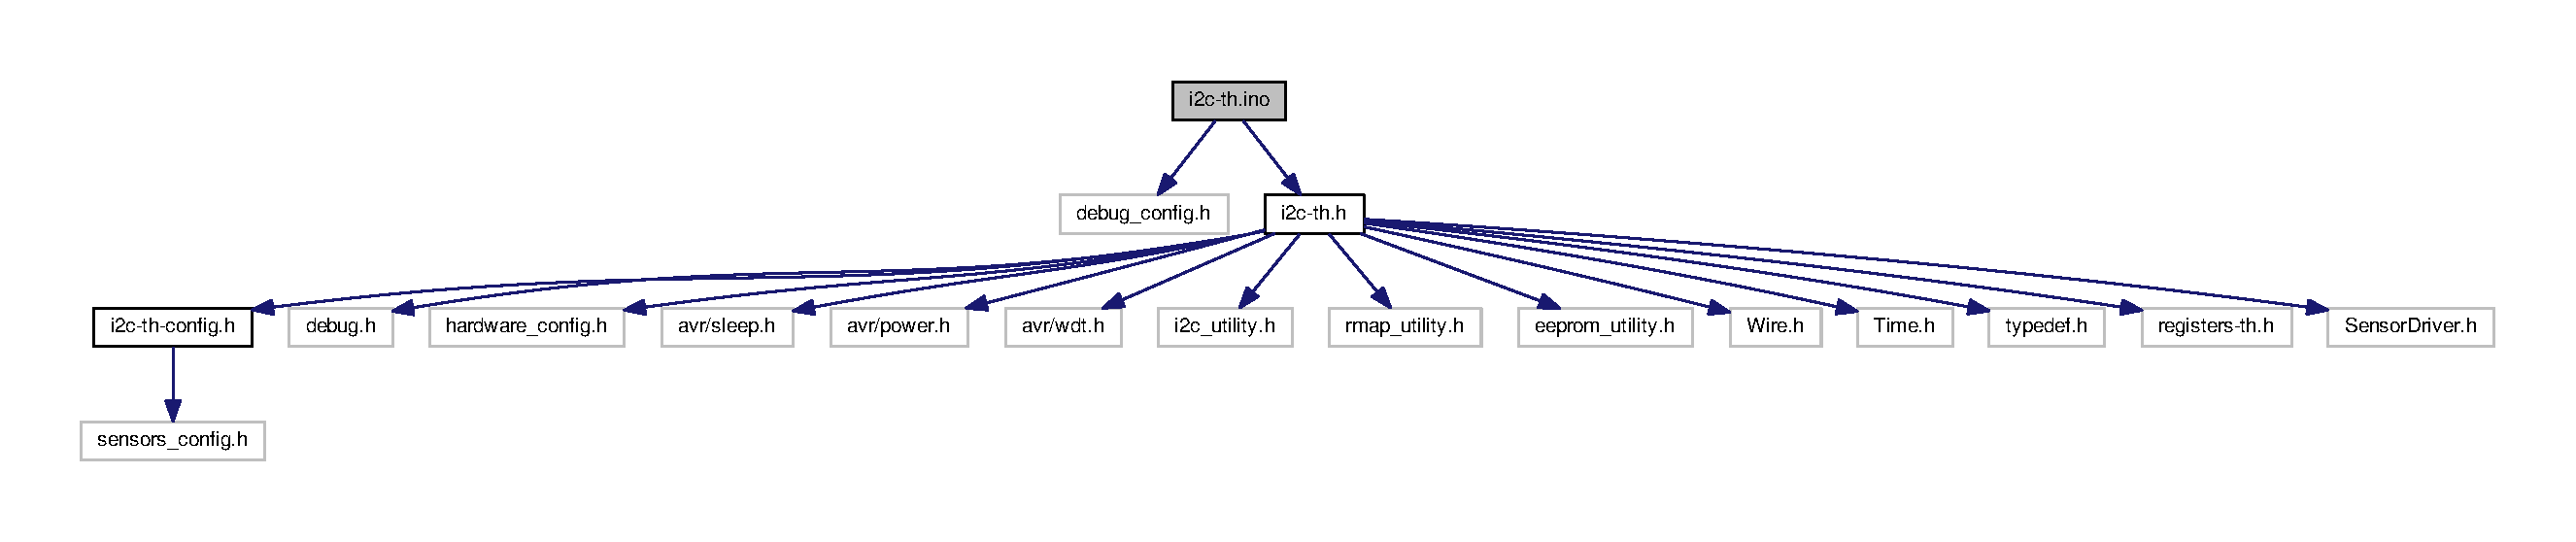
\includegraphics[width=350pt]{i2c-th_8ino__incl}
\end{center}
\end{figure}
\subsection*{Macros}
\begin{DoxyCompactItemize}
\item 
\mbox{\Hypertarget{i2c-th_8ino_a31fa5c36fa17c66feec7a67b76c3e786}\label{i2c-th_8ino_a31fa5c36fa17c66feec7a67b76c3e786}} 
\#define \hyperlink{i2c-th_8ino_a31fa5c36fa17c66feec7a67b76c3e786}{S\+E\+R\+I\+A\+L\+\_\+\+T\+R\+A\+C\+E\+\_\+\+L\+E\+V\+EL}~\hyperlink{debug__config_8h_a0138759b880270bd48d1f329c5c0af4d}{I2\+C\+\_\+\+T\+H\+\_\+\+S\+E\+R\+I\+A\+L\+\_\+\+T\+R\+A\+C\+E\+\_\+\+L\+E\+V\+EL}
\begin{DoxyCompactList}\small\item\em Serial debug level for this sketch. \end{DoxyCompactList}\end{DoxyCompactItemize}
\subsection*{Functions}
\begin{DoxyCompactItemize}
\item 
\mbox{\Hypertarget{i2c-th_8ino_a4fc01d736fe50cf5b977f755b675f11d}\label{i2c-th_8ino_a4fc01d736fe50cf5b977f755b675f11d}} 
void {\bfseries setup} ()
\item 
\mbox{\Hypertarget{i2c-th_8ino_afe461d27b9c48d5921c00d521181f12f}\label{i2c-th_8ino_afe461d27b9c48d5921c00d521181f12f}} 
void {\bfseries loop} ()
\item 
void \hyperlink{i2c-th_8ino_afb98a0f07c30784284f48271ffe02b97}{init\+\_\+power\+\_\+down} (uint32\+\_\+t $\ast$time\+\_\+ms, uint32\+\_\+t debouncing\+\_\+ms)
\begin{DoxyCompactList}\small\item\em Enter power down mode. \end{DoxyCompactList}\item 
void \hyperlink{i2c-th_8ino_a980e73df66b14b1190bc25da430a4f12}{init\+\_\+wdt} (uint8\+\_\+t wdt\+\_\+timer)
\begin{DoxyCompactList}\small\item\em Init watchdog. \end{DoxyCompactList}\item 
void \hyperlink{i2c-th_8ino_ad241cc00b1a92e6d85827df96778e442}{init\+\_\+buffers} ()
\begin{DoxyCompactList}\small\item\em Init buffers. \end{DoxyCompactList}\item 
void \hyperlink{i2c-th_8ino_ab4bf0a3d77da083f131d3fa35a37d2b1}{init\+\_\+tasks} ()
\begin{DoxyCompactList}\small\item\em Init tasks variable and state. \end{DoxyCompactList}\item 
void \hyperlink{i2c-th_8ino_ad8b80a0c08f928106018edd6ea435b95}{init\+\_\+pins} ()
\begin{DoxyCompactList}\small\item\em Init hardware pins. \end{DoxyCompactList}\item 
void \hyperlink{i2c-th_8ino_a2441543100bf8421f56edd622a2c1d9a}{init\+\_\+wire} ()
\begin{DoxyCompactList}\small\item\em Init wire (i2c) library and performs checks on the bus. \end{DoxyCompactList}\item 
void \hyperlink{i2c-th_8ino_a8eb9780a3438ec02c70314744f91f3c7}{init\+\_\+spi} ()
\begin{DoxyCompactList}\small\item\em Init S\+PI library. \end{DoxyCompactList}\item 
void \hyperlink{i2c-th_8ino_ab985cc69f5f573113405b4f118c96d33}{init\+\_\+rtc} ()
\begin{DoxyCompactList}\small\item\em Init R\+TC module. \end{DoxyCompactList}\item 
void \hyperlink{i2c-th_8ino_afceb890a6ab9be73cc5481369538c705}{init\+\_\+system} ()
\begin{DoxyCompactList}\small\item\em Init system. \end{DoxyCompactList}\item 
void \hyperlink{i2c-th_8ino_a65b2dadc0411e43874ec8ed7f73bc62a}{print\+\_\+configuration} ()
\begin{DoxyCompactList}\small\item\em Print current configuration. \end{DoxyCompactList}\item 
void \hyperlink{i2c-th_8ino_afa979a8cb238fe81bf20654dfd6096ef}{save\+\_\+configuration} (bool is\+\_\+default)
\begin{DoxyCompactList}\small\item\em Save configuration to E\+E\+P\+R\+OM. \end{DoxyCompactList}\item 
void \hyperlink{i2c-th_8ino_a32a64a2800c724fb28e10636f2ec20b9}{load\+\_\+configuration} ()
\begin{DoxyCompactList}\small\item\em Load configuration from E\+E\+P\+R\+OM. \end{DoxyCompactList}\item 
void \hyperlink{i2c-th_8ino_ac74850003fab6eb3269bfe043d0f939c}{init\+\_\+sensors} ()
\begin{DoxyCompactList}\small\item\em Create and setup sensors. \end{DoxyCompactList}\item 
\hyperlink{i2c-th_8ino_ab16889ae984b9b798989a0d239283cac}{I\+SR} (T\+I\+M\+E\+R1\+\_\+\+O\+V\+F\+\_\+vect)
\begin{DoxyCompactList}\small\item\em Timer1 overflow interrupts routine. \end{DoxyCompactList}\item 
void \hyperlink{i2c-th_8ino_ac816bd8aafe77e7a571574c8a26eead5}{i2c\+\_\+request\+\_\+interrupt\+\_\+handler} ()
\begin{DoxyCompactList}\small\item\em I2C request interrupt handler. \end{DoxyCompactList}\item 
void \hyperlink{i2c-th_8ino_a6e27532df66f6bf186654355def5c9af}{i2c\+\_\+receive\+\_\+interrupt\+\_\+handler} (int rx\+\_\+data\+\_\+length)
\item 
bool \hyperlink{i2c-th_8ino_a1c5769e114267b210fb3812064d01dd0}{make\+\_\+observation\+\_\+from\+\_\+samples} (bool is\+\_\+force\+\_\+processing, \hyperlink{structsample__t}{sample\+\_\+t} $\ast$sample, \hyperlink{structobservation__t}{observation\+\_\+t} $\ast$observation)
\begin{DoxyCompactList}\small\item\em Processing the samples to calculate an observation when the number of the samples reaches the exact samples\+\_\+count value. \end{DoxyCompactList}\item 
void \hyperlink{i2c-th_8ino_aba0fc91d6c2829df00a9d5fe2b921c90}{samples\+\_\+processing} (bool is\+\_\+force\+\_\+processing)
\begin{DoxyCompactList}\small\item\em Main routine for processing the samples to calculate an observation. \end{DoxyCompactList}\item 
bool \hyperlink{i2c-th_8ino_ab301e4d552826ef91458f52963949a1d}{make\+\_\+value\+\_\+from\+\_\+samples\+\_\+and\+\_\+observations} (\hyperlink{structsample__t}{sample\+\_\+t} $\ast$sample, \hyperlink{structobservation__t}{observation\+\_\+t} $\ast$observation, volatile \hyperlink{structvalue__t}{value\+\_\+t} $\ast$value)
\begin{DoxyCompactList}\small\item\em Processing the observations to calculate a value for report when the number of the observations reaches the minimum value of S\+T\+A\+T\+I\+S\+T\+I\+C\+A\+L\+\_\+\+D\+A\+T\+A\+\_\+\+C\+O\+U\+NT. \end{DoxyCompactList}\item 
void \hyperlink{i2c-th_8ino_a4c8e037e3b3f4c043abf3de8cf57fe68}{observations\+\_\+processing} ()
\begin{DoxyCompactList}\small\item\em Main routine for processing the observations to calculate a value for report. \end{DoxyCompactList}\item 
void \hyperlink{i2c-th_8ino_ad3efe51e17cb8205a24267c2992a12d4}{sensors\+\_\+reading\+\_\+task} ()
\begin{DoxyCompactList}\small\item\em Sensors reading Task. Read data from sensors. \end{DoxyCompactList}\item 
void \hyperlink{i2c-th_8ino_a46696a96b3118b5d8900703c054166c8}{exchange\+\_\+buffers} ()
\begin{DoxyCompactList}\small\item\em Exchange reader and writer pointer to buffer. \end{DoxyCompactList}\item 
void \hyperlink{i2c-th_8ino_ae176339df7451dc03037f319710575aa}{reset\+\_\+samples\+\_\+buffer} ()
\begin{DoxyCompactList}\small\item\em Reset samples buffers to default value. \end{DoxyCompactList}\item 
void \hyperlink{i2c-th_8ino_adfc6b4ac31f79cb1c99dd2409f05f32d}{reset\+\_\+observations\+\_\+buffer} ()
\begin{DoxyCompactList}\small\item\em Reset observations buffers to default value. \end{DoxyCompactList}\item 
void \hyperlink{i2c-th_8ino_a42389aceb96a84573eb67e6d141cb594}{command\+\_\+task} ()
\begin{DoxyCompactList}\small\item\em Execute the command received on i2c bus by reading i2c received data buffer. \end{DoxyCompactList}\item 
void \hyperlink{i2c-th_8ino_a4981066e183f1432ffd6eddf55826585}{commands} ()
\begin{DoxyCompactList}\small\item\em Performs specific operations based on the received command. \end{DoxyCompactList}\end{DoxyCompactItemize}


\subsection{Function Documentation}
\mbox{\Hypertarget{i2c-th_8ino_a42389aceb96a84573eb67e6d141cb594}\label{i2c-th_8ino_a42389aceb96a84573eb67e6d141cb594}} 
\index{i2c-\/th.\+ino@{i2c-\/th.\+ino}!command\+\_\+task@{command\+\_\+task}}
\index{command\+\_\+task@{command\+\_\+task}!i2c-\/th.\+ino@{i2c-\/th.\+ino}}
\subsubsection{\texorpdfstring{command\+\_\+task()}{command\_task()}}
{\footnotesize\ttfamily void command\+\_\+task (\begin{DoxyParamCaption}\item[{void}]{ }\end{DoxyParamCaption})}



Execute the command received on i2c bus by reading i2c received data buffer. 

Command Task. Execute the command received on i2c bus by reading i2c received data buffer.

\begin{DoxyReturn}{Returns}
void. 
\end{DoxyReturn}
\mbox{\Hypertarget{i2c-th_8ino_a4981066e183f1432ffd6eddf55826585}\label{i2c-th_8ino_a4981066e183f1432ffd6eddf55826585}} 
\index{i2c-\/th.\+ino@{i2c-\/th.\+ino}!commands@{commands}}
\index{commands@{commands}!i2c-\/th.\+ino@{i2c-\/th.\+ino}}
\subsubsection{\texorpdfstring{commands()}{commands()}}
{\footnotesize\ttfamily void commands (\begin{DoxyParamCaption}\item[{void}]{ }\end{DoxyParamCaption})}



Performs specific operations based on the received command. 

\begin{DoxyReturn}{Returns}
void. 
\end{DoxyReturn}
C\+O\+N\+T\+I\+N\+U\+O\+US S\+T\+A\+RT

C\+O\+N\+T\+I\+N\+U\+O\+US S\+T\+OP

C\+O\+N\+T\+I\+N\+U\+O\+US S\+T\+A\+R\+T-\/\+S\+T\+OP

O\+N\+E\+S\+H\+OT S\+T\+A\+RT

O\+N\+E\+S\+H\+OT S\+T\+OP

O\+N\+E\+S\+H\+OT S\+T\+A\+R\+T-\/\+S\+T\+OP \mbox{\Hypertarget{i2c-th_8ino_a46696a96b3118b5d8900703c054166c8}\label{i2c-th_8ino_a46696a96b3118b5d8900703c054166c8}} 
\index{i2c-\/th.\+ino@{i2c-\/th.\+ino}!exchange\+\_\+buffers@{exchange\+\_\+buffers}}
\index{exchange\+\_\+buffers@{exchange\+\_\+buffers}!i2c-\/th.\+ino@{i2c-\/th.\+ino}}
\subsubsection{\texorpdfstring{exchange\+\_\+buffers()}{exchange\_buffers()}}
{\footnotesize\ttfamily void exchange\+\_\+buffers (\begin{DoxyParamCaption}\item[{void}]{ }\end{DoxyParamCaption})}



Exchange reader and writer pointer to buffer. 

\begin{DoxyReturn}{Returns}
void. 
\end{DoxyReturn}
\mbox{\Hypertarget{i2c-th_8ino_a6e27532df66f6bf186654355def5c9af}\label{i2c-th_8ino_a6e27532df66f6bf186654355def5c9af}} 
\index{i2c-\/th.\+ino@{i2c-\/th.\+ino}!i2c\+\_\+receive\+\_\+interrupt\+\_\+handler@{i2c\+\_\+receive\+\_\+interrupt\+\_\+handler}}
\index{i2c\+\_\+receive\+\_\+interrupt\+\_\+handler@{i2c\+\_\+receive\+\_\+interrupt\+\_\+handler}!i2c-\/th.\+ino@{i2c-\/th.\+ino}}
\subsubsection{\texorpdfstring{i2c\+\_\+receive\+\_\+interrupt\+\_\+handler()}{i2c\_receive\_interrupt\_handler()}}
{\footnotesize\ttfamily void i2c\+\_\+receive\+\_\+interrupt\+\_\+handler (\begin{DoxyParamCaption}\item[{int}]{rx\+\_\+data\+\_\+length }\end{DoxyParamCaption})}

read rx\+\_\+data\+\_\+length bytes of data from i2c bus

it is a registers read?

offset in readable\+\_\+data\+\_\+read\+\_\+ptr buffer

length (in butes) of data to be read in readable\+\_\+data\+\_\+read\+\_\+ptr

it is a command?

enable Command task

it is a registers write?

write rx\+\_\+data\+\_\+length bytes in writable\+\_\+data\+\_\+ptr (base) at (i2c\+\_\+rx\+\_\+data\mbox{[}i\mbox{]} -\/ I2\+C\+\_\+\+W\+R\+I\+T\+E\+\_\+\+R\+E\+G\+I\+S\+T\+E\+R\+\_\+\+S\+T\+A\+R\+T\+\_\+\+A\+D\+D\+R\+E\+SS) (position in buffer) \mbox{\Hypertarget{i2c-th_8ino_ac816bd8aafe77e7a571574c8a26eead5}\label{i2c-th_8ino_ac816bd8aafe77e7a571574c8a26eead5}} 
\index{i2c-\/th.\+ino@{i2c-\/th.\+ino}!i2c\+\_\+request\+\_\+interrupt\+\_\+handler@{i2c\+\_\+request\+\_\+interrupt\+\_\+handler}}
\index{i2c\+\_\+request\+\_\+interrupt\+\_\+handler@{i2c\+\_\+request\+\_\+interrupt\+\_\+handler}!i2c-\/th.\+ino@{i2c-\/th.\+ino}}
\subsubsection{\texorpdfstring{i2c\+\_\+request\+\_\+interrupt\+\_\+handler()}{i2c\_request\_interrupt\_handler()}}
{\footnotesize\ttfamily void i2c\+\_\+request\+\_\+interrupt\+\_\+handler (\begin{DoxyParamCaption}\item[{void}]{ }\end{DoxyParamCaption})}



I2C request interrupt handler. 

\begin{DoxyReturn}{Returns}
void. 
\end{DoxyReturn}
write readable\+\_\+data\+\_\+length bytes of data stored in readable\+\_\+data\+\_\+read\+\_\+ptr (base) + readable\+\_\+data\+\_\+address (offset) on i2c bus \mbox{\Hypertarget{i2c-th_8ino_ad241cc00b1a92e6d85827df96778e442}\label{i2c-th_8ino_ad241cc00b1a92e6d85827df96778e442}} 
\index{i2c-\/th.\+ino@{i2c-\/th.\+ino}!init\+\_\+buffers@{init\+\_\+buffers}}
\index{init\+\_\+buffers@{init\+\_\+buffers}!i2c-\/th.\+ino@{i2c-\/th.\+ino}}
\subsubsection{\texorpdfstring{init\+\_\+buffers()}{init\_buffers()}}
{\footnotesize\ttfamily void init\+\_\+buffers (\begin{DoxyParamCaption}\item[{void}]{ }\end{DoxyParamCaption})}



Init buffers. 

\begin{DoxyReturn}{Returns}
void. 
\end{DoxyReturn}
copy readable\+\_\+data\+\_\+2 in readable\+\_\+data\+\_\+1 \mbox{\Hypertarget{i2c-th_8ino_ad8b80a0c08f928106018edd6ea435b95}\label{i2c-th_8ino_ad8b80a0c08f928106018edd6ea435b95}} 
\index{i2c-\/th.\+ino@{i2c-\/th.\+ino}!init\+\_\+pins@{init\+\_\+pins}}
\index{init\+\_\+pins@{init\+\_\+pins}!i2c-\/th.\+ino@{i2c-\/th.\+ino}}
\subsubsection{\texorpdfstring{init\+\_\+pins()}{init\_pins()}}
{\footnotesize\ttfamily void init\+\_\+pins (\begin{DoxyParamCaption}\item[{void}]{ }\end{DoxyParamCaption})}



Init hardware pins. 

\begin{DoxyReturn}{Returns}
void. 
\end{DoxyReturn}
\mbox{\Hypertarget{i2c-th_8ino_afb98a0f07c30784284f48271ffe02b97}\label{i2c-th_8ino_afb98a0f07c30784284f48271ffe02b97}} 
\index{i2c-\/th.\+ino@{i2c-\/th.\+ino}!init\+\_\+power\+\_\+down@{init\+\_\+power\+\_\+down}}
\index{init\+\_\+power\+\_\+down@{init\+\_\+power\+\_\+down}!i2c-\/th.\+ino@{i2c-\/th.\+ino}}
\subsubsection{\texorpdfstring{init\+\_\+power\+\_\+down()}{init\_power\_down()}}
{\footnotesize\ttfamily void init\+\_\+power\+\_\+down (\begin{DoxyParamCaption}\item[{uint32\+\_\+t $\ast$}]{time\+\_\+ms,  }\item[{uint32\+\_\+t}]{debouncing\+\_\+ms }\end{DoxyParamCaption})}



Enter power down mode. 


\begin{DoxyParams}{Parameters}
{\em time\+\_\+ms} & pointer to a variable to save the last instant you entered power down. \\
\hline
{\em debouncing\+\_\+ms} & delay to power down. \\
\hline
\end{DoxyParams}
\begin{DoxyReturn}{Returns}
void. 
\end{DoxyReturn}
turn off brown-\/out \mbox{\Hypertarget{i2c-th_8ino_ab985cc69f5f573113405b4f118c96d33}\label{i2c-th_8ino_ab985cc69f5f573113405b4f118c96d33}} 
\index{i2c-\/th.\+ino@{i2c-\/th.\+ino}!init\+\_\+rtc@{init\+\_\+rtc}}
\index{init\+\_\+rtc@{init\+\_\+rtc}!i2c-\/th.\+ino@{i2c-\/th.\+ino}}
\subsubsection{\texorpdfstring{init\+\_\+rtc()}{init\_rtc()}}
{\footnotesize\ttfamily void init\+\_\+rtc (\begin{DoxyParamCaption}\item[{void}]{ }\end{DoxyParamCaption})}



Init R\+TC module. 

\begin{DoxyReturn}{Returns}
void. 
\end{DoxyReturn}
\mbox{\Hypertarget{i2c-th_8ino_ac74850003fab6eb3269bfe043d0f939c}\label{i2c-th_8ino_ac74850003fab6eb3269bfe043d0f939c}} 
\index{i2c-\/th.\+ino@{i2c-\/th.\+ino}!init\+\_\+sensors@{init\+\_\+sensors}}
\index{init\+\_\+sensors@{init\+\_\+sensors}!i2c-\/th.\+ino@{i2c-\/th.\+ino}}
\subsubsection{\texorpdfstring{init\+\_\+sensors()}{init\_sensors()}}
{\footnotesize\ttfamily void init\+\_\+sensors (\begin{DoxyParamCaption}\item[{void}]{ }\end{DoxyParamCaption})}



Create and setup sensors. 

\begin{DoxyReturn}{Returns}
void. 
\end{DoxyReturn}
\mbox{\Hypertarget{i2c-th_8ino_a8eb9780a3438ec02c70314744f91f3c7}\label{i2c-th_8ino_a8eb9780a3438ec02c70314744f91f3c7}} 
\index{i2c-\/th.\+ino@{i2c-\/th.\+ino}!init\+\_\+spi@{init\+\_\+spi}}
\index{init\+\_\+spi@{init\+\_\+spi}!i2c-\/th.\+ino@{i2c-\/th.\+ino}}
\subsubsection{\texorpdfstring{init\+\_\+spi()}{init\_spi()}}
{\footnotesize\ttfamily void init\+\_\+spi (\begin{DoxyParamCaption}\item[{void}]{ }\end{DoxyParamCaption})}



Init S\+PI library. 

\begin{DoxyReturn}{Returns}
void. 
\end{DoxyReturn}
\mbox{\Hypertarget{i2c-th_8ino_afceb890a6ab9be73cc5481369538c705}\label{i2c-th_8ino_afceb890a6ab9be73cc5481369538c705}} 
\index{i2c-\/th.\+ino@{i2c-\/th.\+ino}!init\+\_\+system@{init\+\_\+system}}
\index{init\+\_\+system@{init\+\_\+system}!i2c-\/th.\+ino@{i2c-\/th.\+ino}}
\subsubsection{\texorpdfstring{init\+\_\+system()}{init\_system()}}
{\footnotesize\ttfamily void init\+\_\+system (\begin{DoxyParamCaption}\item[{void}]{ }\end{DoxyParamCaption})}



Init system. 

\begin{DoxyReturn}{Returns}
void. 
\end{DoxyReturn}
main loop state \mbox{\Hypertarget{i2c-th_8ino_ab4bf0a3d77da083f131d3fa35a37d2b1}\label{i2c-th_8ino_ab4bf0a3d77da083f131d3fa35a37d2b1}} 
\index{i2c-\/th.\+ino@{i2c-\/th.\+ino}!init\+\_\+tasks@{init\+\_\+tasks}}
\index{init\+\_\+tasks@{init\+\_\+tasks}!i2c-\/th.\+ino@{i2c-\/th.\+ino}}
\subsubsection{\texorpdfstring{init\+\_\+tasks()}{init\_tasks()}}
{\footnotesize\ttfamily void init\+\_\+tasks (\begin{DoxyParamCaption}\item[{void}]{ }\end{DoxyParamCaption})}



Init tasks variable and state. 

\begin{DoxyReturn}{Returns}
void. 
\end{DoxyReturn}
no tasks ready

reset samples\+\_\+count value \mbox{\Hypertarget{i2c-th_8ino_a980e73df66b14b1190bc25da430a4f12}\label{i2c-th_8ino_a980e73df66b14b1190bc25da430a4f12}} 
\index{i2c-\/th.\+ino@{i2c-\/th.\+ino}!init\+\_\+wdt@{init\+\_\+wdt}}
\index{init\+\_\+wdt@{init\+\_\+wdt}!i2c-\/th.\+ino@{i2c-\/th.\+ino}}
\subsubsection{\texorpdfstring{init\+\_\+wdt()}{init\_wdt()}}
{\footnotesize\ttfamily void init\+\_\+wdt (\begin{DoxyParamCaption}\item[{uint8\+\_\+t}]{wdt\+\_\+timer }\end{DoxyParamCaption})}



Init watchdog. 


\begin{DoxyParams}{Parameters}
{\em wdt\+\_\+timer} & a time value for init watchdog (W\+D\+T\+O\+\_\+xxxx). \\
\hline
\end{DoxyParams}
\begin{DoxyReturn}{Returns}
void. 
\end{DoxyReturn}
\mbox{\Hypertarget{i2c-th_8ino_a2441543100bf8421f56edd622a2c1d9a}\label{i2c-th_8ino_a2441543100bf8421f56edd622a2c1d9a}} 
\index{i2c-\/th.\+ino@{i2c-\/th.\+ino}!init\+\_\+wire@{init\+\_\+wire}}
\index{init\+\_\+wire@{init\+\_\+wire}!i2c-\/th.\+ino@{i2c-\/th.\+ino}}
\subsubsection{\texorpdfstring{init\+\_\+wire()}{init\_wire()}}
{\footnotesize\ttfamily void init\+\_\+wire (\begin{DoxyParamCaption}\item[{void}]{ }\end{DoxyParamCaption})}



Init wire (i2c) library and performs checks on the bus. 

\begin{DoxyReturn}{Returns}
void. 
\end{DoxyReturn}
clear the I2C bus first before calling Wire.\+begin()

wait for watchdog reboot \mbox{\Hypertarget{i2c-th_8ino_ab16889ae984b9b798989a0d239283cac}\label{i2c-th_8ino_ab16889ae984b9b798989a0d239283cac}} 
\index{i2c-\/th.\+ino@{i2c-\/th.\+ino}!I\+SR@{I\+SR}}
\index{I\+SR@{I\+SR}!i2c-\/th.\+ino@{i2c-\/th.\+ino}}
\subsubsection{\texorpdfstring{I\+S\+R()}{ISR()}}
{\footnotesize\ttfamily I\+SR (\begin{DoxyParamCaption}\item[{T\+I\+M\+E\+R1\+\_\+\+O\+V\+F\+\_\+vect}]{ }\end{DoxyParamCaption})}



Timer1 overflow interrupts routine. 

\begin{DoxyReturn}{Returns}
void. 
\end{DoxyReturn}
Pre-\/load timer counter register

increment timer\+\_\+counter by T\+I\+M\+E\+R1\+\_\+\+I\+N\+T\+E\+R\+R\+U\+P\+T\+\_\+\+T\+I\+M\+E\+\_\+\+MS

check if S\+E\+N\+S\+O\+R\+S\+\_\+\+S\+A\+M\+P\+L\+E\+\_\+\+T\+I\+M\+E\+\_\+\+MS ms have passed since last time. if true and if is in continuous mode and continuous start command It has been received, activate Sensor reading task

reset timer\+\_\+counter if it has become larger than T\+I\+M\+E\+R1\+\_\+\+V\+A\+L\+U\+E\+\_\+\+M\+A\+X\+\_\+\+MS \mbox{\Hypertarget{i2c-th_8ino_a32a64a2800c724fb28e10636f2ec20b9}\label{i2c-th_8ino_a32a64a2800c724fb28e10636f2ec20b9}} 
\index{i2c-\/th.\+ino@{i2c-\/th.\+ino}!load\+\_\+configuration@{load\+\_\+configuration}}
\index{load\+\_\+configuration@{load\+\_\+configuration}!i2c-\/th.\+ino@{i2c-\/th.\+ino}}
\subsubsection{\texorpdfstring{load\+\_\+configuration()}{load\_configuration()}}
{\footnotesize\ttfamily void load\+\_\+configuration (\begin{DoxyParamCaption}\item[{void}]{ }\end{DoxyParamCaption})}



Load configuration from E\+E\+P\+R\+OM. 

\begin{DoxyReturn}{Returns}
void. 
\end{DoxyReturn}
read configuration from eeprom \mbox{\Hypertarget{i2c-th_8ino_a1c5769e114267b210fb3812064d01dd0}\label{i2c-th_8ino_a1c5769e114267b210fb3812064d01dd0}} 
\index{i2c-\/th.\+ino@{i2c-\/th.\+ino}!make\+\_\+observation\+\_\+from\+\_\+samples@{make\+\_\+observation\+\_\+from\+\_\+samples}}
\index{make\+\_\+observation\+\_\+from\+\_\+samples@{make\+\_\+observation\+\_\+from\+\_\+samples}!i2c-\/th.\+ino@{i2c-\/th.\+ino}}
\subsubsection{\texorpdfstring{make\+\_\+observation\+\_\+from\+\_\+samples()}{make\_observation\_from\_samples()}}
{\footnotesize\ttfamily bool make\+\_\+observation\+\_\+from\+\_\+samples (\begin{DoxyParamCaption}\item[{bool}]{is\+\_\+force\+\_\+processing,  }\item[{\hyperlink{structsample__t}{sample\+\_\+t} $\ast$}]{sample,  }\item[{\hyperlink{structobservation__t}{observation\+\_\+t} $\ast$}]{observation }\end{DoxyParamCaption})}



Processing the samples to calculate an observation when the number of the samples reaches the exact samples\+\_\+count value. 


\begin{DoxyParams}{Parameters}
{\em is\+\_\+force\+\_\+processing} & if is true, force the calculation of the observation provided there is a minimum number of samples. \\
\hline
{\em $\ast$sample} & input samples. \\
\hline
{\em $\ast$observation} & output observation. \\
\hline
\end{DoxyParams}
\begin{DoxyReturn}{Returns}
void. 
\end{DoxyReturn}
default value for observation

when true, indicates that sufficient samples have been acquired for the calculation of an observation (except for samples errors)

force processing when samples\+\_\+count = S\+E\+N\+S\+O\+R\+S\+\_\+\+S\+A\+M\+P\+L\+E\+\_\+\+C\+O\+U\+N\+T\+\_\+\+M\+AX

force processing when samples\+\_\+count = S\+E\+N\+S\+O\+R\+S\+\_\+\+S\+A\+M\+P\+L\+E\+\_\+\+C\+O\+U\+N\+T\+\_\+\+M\+IN

normal behavior\+: processing when correct measure sample count + error measure sample count == samples\+\_\+count

if true, indicates that there are good enough samples for the calculation of observation

if true, you can calculate the observation

sum all good samples

calculate average of all good samples

assign a observation buffer with current value \mbox{\Hypertarget{i2c-th_8ino_ab301e4d552826ef91458f52963949a1d}\label{i2c-th_8ino_ab301e4d552826ef91458f52963949a1d}} 
\index{i2c-\/th.\+ino@{i2c-\/th.\+ino}!make\+\_\+value\+\_\+from\+\_\+samples\+\_\+and\+\_\+observations@{make\+\_\+value\+\_\+from\+\_\+samples\+\_\+and\+\_\+observations}}
\index{make\+\_\+value\+\_\+from\+\_\+samples\+\_\+and\+\_\+observations@{make\+\_\+value\+\_\+from\+\_\+samples\+\_\+and\+\_\+observations}!i2c-\/th.\+ino@{i2c-\/th.\+ino}}
\subsubsection{\texorpdfstring{make\+\_\+value\+\_\+from\+\_\+samples\+\_\+and\+\_\+observations()}{make\_value\_from\_samples\_and\_observations()}}
{\footnotesize\ttfamily bool make\+\_\+value\+\_\+from\+\_\+samples\+\_\+and\+\_\+observations (\begin{DoxyParamCaption}\item[{\hyperlink{structsample__t}{sample\+\_\+t} $\ast$}]{sample,  }\item[{\hyperlink{structobservation__t}{observation\+\_\+t} $\ast$}]{observation,  }\item[{volatile \hyperlink{structvalue__t}{value\+\_\+t} $\ast$}]{value }\end{DoxyParamCaption})}



Processing the observations to calculate a value for report when the number of the observations reaches the minimum value of S\+T\+A\+T\+I\+S\+T\+I\+C\+A\+L\+\_\+\+D\+A\+T\+A\+\_\+\+C\+O\+U\+NT. 


\begin{DoxyParams}{Parameters}
{\em $\ast$sample} & input samples. \\
\hline
{\em $\ast$observation} & input observation. \\
\hline
{\em $\ast$value} & output value for report. \\
\hline
\end{DoxyParams}
\begin{DoxyReturn}{Returns}
void. 
\end{DoxyReturn}
new read pointer in circular observation buffer

temporary write pointer in circular observation buffer

temporary value

good observation counter

error observation counter

standard deviation

counter of the number of observation in memory

if true, you can calculate the value for report (there are at least S\+T\+A\+T\+I\+S\+T\+I\+C\+A\+L\+\_\+\+D\+A\+T\+A\+\_\+\+C\+O\+U\+NT observations)

initialize write ptr

calculate write\+\_\+ptr\+: if the end is reached, reset to the first address, else increment by one

reset value to default

loop until I have finished processing the last S\+T\+A\+T\+I\+S\+T\+I\+C\+A\+L\+\_\+\+D\+A\+T\+A\+\_\+\+C\+O\+U\+NT observations

if it is a good observation, calculate sum, minimum and maximum value. Otherwise increment error counter.

assign minimum to report value

assign maximum to report value

calculate read\+\_\+ptr\+: if the end is reached, reset to the first address, else increment by one

calculate next read\+\_\+ptr (observation-\/$>$write\+\_\+ptr + 1 for pre-\/calculate next processing)

assign read\+\_\+ptr to new next value

assign last sample to report value

assign last observation to report value

calculate observations average only if there are enough good observations

calculate standard deviation

loop until I have finished processing the last S\+T\+A\+T\+I\+S\+T\+I\+C\+A\+L\+\_\+\+D\+A\+T\+A\+\_\+\+C\+O\+U\+NT observations

if it is a good observation, calculate variance

calculate read\+\_\+ptr\+: if the end is reached, reset to the first address, else increment by one

calculate standard deviation only if there are enough good observations

calculate next read\+\_\+ptr (observation-\/$>$write\+\_\+ptr + 1 for pre-\/calculate next processing)

assign read\+\_\+ptr to new next value \mbox{\Hypertarget{i2c-th_8ino_a4c8e037e3b3f4c043abf3de8cf57fe68}\label{i2c-th_8ino_a4c8e037e3b3f4c043abf3de8cf57fe68}} 
\index{i2c-\/th.\+ino@{i2c-\/th.\+ino}!observations\+\_\+processing@{observations\+\_\+processing}}
\index{observations\+\_\+processing@{observations\+\_\+processing}!i2c-\/th.\+ino@{i2c-\/th.\+ino}}
\subsubsection{\texorpdfstring{observations\+\_\+processing()}{observations\_processing()}}
{\footnotesize\ttfamily void observations\+\_\+processing (\begin{DoxyParamCaption}\item[{void}]{ }\end{DoxyParamCaption})}



Main routine for processing the observations to calculate a value for report. 

\begin{DoxyReturn}{Returns}
void. 
\end{DoxyReturn}
if true, a new temperature report was calculated

if true, a new humidty report was calculated

reset buffer of samples value \mbox{\Hypertarget{i2c-th_8ino_a65b2dadc0411e43874ec8ed7f73bc62a}\label{i2c-th_8ino_a65b2dadc0411e43874ec8ed7f73bc62a}} 
\index{i2c-\/th.\+ino@{i2c-\/th.\+ino}!print\+\_\+configuration@{print\+\_\+configuration}}
\index{print\+\_\+configuration@{print\+\_\+configuration}!i2c-\/th.\+ino@{i2c-\/th.\+ino}}
\subsubsection{\texorpdfstring{print\+\_\+configuration()}{print\_configuration()}}
{\footnotesize\ttfamily void print\+\_\+configuration (\begin{DoxyParamCaption}\item[{void}]{ }\end{DoxyParamCaption})}



Print current configuration. 

\begin{DoxyReturn}{Returns}
void. 
\end{DoxyReturn}
\mbox{\Hypertarget{i2c-th_8ino_adfc6b4ac31f79cb1c99dd2409f05f32d}\label{i2c-th_8ino_adfc6b4ac31f79cb1c99dd2409f05f32d}} 
\index{i2c-\/th.\+ino@{i2c-\/th.\+ino}!reset\+\_\+observations\+\_\+buffer@{reset\+\_\+observations\+\_\+buffer}}
\index{reset\+\_\+observations\+\_\+buffer@{reset\+\_\+observations\+\_\+buffer}!i2c-\/th.\+ino@{i2c-\/th.\+ino}}
\subsubsection{\texorpdfstring{reset\+\_\+observations\+\_\+buffer()}{reset\_observations\_buffer()}}
{\footnotesize\ttfamily void reset\+\_\+observations\+\_\+buffer (\begin{DoxyParamCaption}\item[{void}]{ }\end{DoxyParamCaption})}



Reset observations buffers to default value. 

\begin{DoxyReturn}{Returns}
void. 
\end{DoxyReturn}
\mbox{\Hypertarget{i2c-th_8ino_ae176339df7451dc03037f319710575aa}\label{i2c-th_8ino_ae176339df7451dc03037f319710575aa}} 
\index{i2c-\/th.\+ino@{i2c-\/th.\+ino}!reset\+\_\+samples\+\_\+buffer@{reset\+\_\+samples\+\_\+buffer}}
\index{reset\+\_\+samples\+\_\+buffer@{reset\+\_\+samples\+\_\+buffer}!i2c-\/th.\+ino@{i2c-\/th.\+ino}}
\subsubsection{\texorpdfstring{reset\+\_\+samples\+\_\+buffer()}{reset\_samples\_buffer()}}
{\footnotesize\ttfamily void reset\+\_\+samples\+\_\+buffer (\begin{DoxyParamCaption}\item[{void}]{ }\end{DoxyParamCaption})}



Reset samples buffers to default value. 

\begin{DoxyReturn}{Returns}
void. 
\end{DoxyReturn}
\mbox{\Hypertarget{i2c-th_8ino_aba0fc91d6c2829df00a9d5fe2b921c90}\label{i2c-th_8ino_aba0fc91d6c2829df00a9d5fe2b921c90}} 
\index{i2c-\/th.\+ino@{i2c-\/th.\+ino}!samples\+\_\+processing@{samples\+\_\+processing}}
\index{samples\+\_\+processing@{samples\+\_\+processing}!i2c-\/th.\+ino@{i2c-\/th.\+ino}}
\subsubsection{\texorpdfstring{samples\+\_\+processing()}{samples\_processing()}}
{\footnotesize\ttfamily void samples\+\_\+processing (\begin{DoxyParamCaption}\item[{bool}]{is\+\_\+force\+\_\+processing }\end{DoxyParamCaption})}



Main routine for processing the samples to calculate an observation. 


\begin{DoxyParams}{Parameters}
{\em is\+\_\+force\+\_\+processing} & if is true, force the calculation of the observation provided there is a minimum number of samples. \\
\hline
\end{DoxyParams}
\begin{DoxyReturn}{Returns}
void. 
\end{DoxyReturn}
if true, a new temperature observation was calculated

if true, a new humidity observation was calculated

assign new value for samples\+\_\+count \mbox{\Hypertarget{i2c-th_8ino_afa979a8cb238fe81bf20654dfd6096ef}\label{i2c-th_8ino_afa979a8cb238fe81bf20654dfd6096ef}} 
\index{i2c-\/th.\+ino@{i2c-\/th.\+ino}!save\+\_\+configuration@{save\+\_\+configuration}}
\index{save\+\_\+configuration@{save\+\_\+configuration}!i2c-\/th.\+ino@{i2c-\/th.\+ino}}
\subsubsection{\texorpdfstring{save\+\_\+configuration()}{save\_configuration()}}
{\footnotesize\ttfamily void save\+\_\+configuration (\begin{DoxyParamCaption}\item[{bool}]{is\+\_\+default }\end{DoxyParamCaption})}



Save configuration to E\+E\+P\+R\+OM. 


\begin{DoxyParams}{Parameters}
{\em is\+\_\+default} & if true save default configuration; if false save current configuration. \\
\hline
\end{DoxyParams}
\begin{DoxyReturn}{Returns}
void. 
\end{DoxyReturn}
write configuration to eeprom \mbox{\Hypertarget{i2c-th_8ino_ad3efe51e17cb8205a24267c2992a12d4}\label{i2c-th_8ino_ad3efe51e17cb8205a24267c2992a12d4}} 
\index{i2c-\/th.\+ino@{i2c-\/th.\+ino}!sensors\+\_\+reading\+\_\+task@{sensors\+\_\+reading\+\_\+task}}
\index{sensors\+\_\+reading\+\_\+task@{sensors\+\_\+reading\+\_\+task}!i2c-\/th.\+ino@{i2c-\/th.\+ino}}
\subsubsection{\texorpdfstring{sensors\+\_\+reading\+\_\+task()}{sensors\_reading\_task()}}
{\footnotesize\ttfamily void sensors\+\_\+reading\+\_\+task (\begin{DoxyParamCaption}\item[{void}]{ }\end{DoxyParamCaption})}



Sensors reading Task. Read data from sensors. 

\begin{DoxyReturn}{Returns}
void. 
\end{DoxyReturn}
reset internal state of all sensors to default

prepare sensor and get delay for complete operation

if there is any delay, wait it. Otherwise go to next.

success

retry

fail

get V\+A\+L\+U\+E\+S\+\_\+\+T\+O\+\_\+\+R\+E\+A\+D\+\_\+\+F\+R\+O\+M\+\_\+\+S\+E\+N\+S\+O\+R\+\_\+\+C\+O\+U\+NT values from sensor and store it in values\+\_\+readed\+\_\+from\+\_\+sensor.

end of internal sensor state (finished read)

success

retry

fail

mark error

go to next sensor

process other internal sensor state

read sensor value

go to next sensor

end (there are no other sensors to read)

if it is in continuous mode, do samples processing 
%--- End generated contents ---

% Index
\backmatter
\newpage
\phantomsection
\clearemptydoublepage
\addcontentsline{toc}{chapter}{Index}
\printindex

\end{document}
